\selectlanguage{english}

\chapter{Algorithms} \label{app1}

\minitoc

\section{Reject inference methods} \label{app1:reject}

\subsection{Fuzzy augmentation} \label{fuzzy}

Fuzzy augmentation can be found in \cite{economix}; it is the following procedure:
\begin{enumerate}
\item Construct Scorecard ``Known Good Bad'' (KGB) $\hat{\gls{bth}}_\f$ with financed clients' data (Figure \ref{fuzzy:sfig1});
\item Calculate $p_{\hat{\gls{bth}}_{\f}}(1|\gls{bbx}_{\nf})$ for rejects (Figure \ref{fuzzy:sfig2});
\item Infer rejected client $i$ as good with weight $p_{\hat{\gls{bth}}_{\text{f}}}(1|\gls{bbx}_{\nf})$ and as bad with weight {\begin{sloppypar} $1-p_{\hat{\gls{bth}}_{\text{f}}}(1|\gls{bbx}_{\nf})$ (Figures \ref{fuzzy:sfig2} and \ref{fuzzy:sfig3}) \end{sloppypar} };
\item Calibrate a new scorecard with the ``augmented'' dataset (Figure \ref{fuzzy:sfig4}).
\end{enumerate}

\begin{table}
\caption{\label{fuzzyexample} Example of implementation of the Fuzzy Augmentation method on a small dataset}
{\setlength{\parindent}{0cm}
\begin{multicols}{4}
\small

\begin{subfigure}[t]{0.22\textwidth}
\begin{center}
\begin{adjustbox}{max width=0.95\textwidth}
\begin{tabular}{l l}
\toprule
\textbf{${\gls{bby}}_{\f}$} & \textbf{${\gls{bbx}}_{\f}$}\\
\midrule
1 & 0.562 \\
1 & 0.910 \\
0 & 0.430 \\
\bottomrule
\end{tabular}
\end{adjustbox}
\end{center}

\subcaption{Scorecard $\hat{\gls{bth}}_\f$ on financed loans}
\label{fuzzy:sfig1}
\end{subfigure}

\columnbreak

\begin{subfigure}[t]{0.22\textwidth}
\begin{center}
\begin{adjustbox}{max width=0.95\textwidth}
\begin{tabular}{l l l}
\toprule
\textbf{Weight} & \textbf{$\hat{\gls{bby}}_{\nf}$} & \textbf{${\gls{bbx}}_{\nf}$}\\
\midrule
0.68 & 1 & 0.347 \\
0.10 & 1 & 0.140 \\
0.35 & 1 & 0.295 \\
\bottomrule
\end{tabular}
\end{adjustbox}
\end{center}

\caption{Inferred good not financed loans and their weights}
\label{fuzzy:sfig2}
\end{subfigure}

\columnbreak

\begin{subfigure}[t]{0.22\textwidth}
\begin{center}
\begin{adjustbox}{max width=0.95\textwidth}
\begin{tabular}{l l l}
\toprule
\textbf{Weight} & \textbf{$\hat{\gls{bby}}_{\nf}$} & \textbf{${\gls{bbx}}_{\nf}$}\\
\midrule
0.32 & 0 & 0.347 \\
0.90 & 0 & 0.140 \\
0.65 & 0 & 0.295 \\
\bottomrule
\end{tabular}
\end{adjustbox}
\end{center}

\caption{Inferred bad not financed loans and their weights}
\label{fuzzy:sfig3}
\end{subfigure}

\columnbreak

\begin{subfigure}[t]{0.22\textwidth}
\begin{center}
\begin{adjustbox}{max width=0.95\textwidth}
\begin{tabular}{l l l}
\toprule
\textbf{Weight} & \textbf{${\gls{bby}}$} & \textbf{${\gls{bbx}}$}\\
\midrule
1 & 0 & 0.562 \\
1 & 1 & 0.910 \\
1 & 0 & 0.430 \\
0.68 & 1 & 0.347 \\
0.10 & 1 & 0.140 \\
0.35 & 1 & 0.295 \\
0.32 & 0 & 0.347 \\
0.90 & 0 & 0.140 \\
0.65 & 0 & 0.295 \\
\bottomrule
\end{tabular}
\end{adjustbox}
\end{center}
\caption{Fuzzy augmented learning dataset}
\label{fuzzy:sfig4}
\end{subfigure}

\end{multicols}
}
\end{table}

Clearly:

\[ \forall j = 1, \ldots, d, \: \frac{\partial \sum_{i=n+1}^{m+n} \sum_{y_i = 0}^{1} p_{\hat{\gls{bth}}_\f}(\gls{y}_i| \gls{bx}_i)\ln (p_{\gls{bth}}(\gls{y}_i| \gls{bx}_i))}{\partial \theta_j} = 0 \Leftrightarrow \theta = \hat{\gls{bth}}_{\f}, \]

such that:
\[\argmax_{\gls{bth} \in \Theta}  \sum_{i=n+1}^{m+n} \sum_{y_i = 0}^{1} p_{\hat{\gls{bth}}_{\f}}(y_i| \gls{bx}_i)\ln (p_{\gls{bth}}(y_i| \gls{bx}_i)) = \hat{\gls{bth}}_{\f},\]

and finally:
\[\argmax_{\gls{bth} \in \Theta} \ell(\gls{bth};\mathcal{T}_{c}) = \argmax_{\gls{bth} \in \Theta} \ell(\gls{bth};\gls{Tf}) = \hat{\gls{bth}}_{\f}. \]

 To conclude, this method will not change the estimated parameters of any discriminant model, asymptotically and with a finite set of observations, regardless of any assumption on the missingness mechanism or the true model hypothesis. In other words, Fuzzy Augmentation has no effect on the $\gls{KL}$ divergence, making this method useless because it is no different than the financed clients model.


\subsection{Reclassification} \label{reclassification}

Reclassification can be found in \cite{RI6}, also sometimes referred to as extrapolation as in \cite{banasik}; it is the following procedure:
\begin{enumerate}
\item Construct Scorecard ``Known Good Bad'' (KGB) $\hat{\gls{bth}}_{\text{f}}$ with financed clients' data (Figure~\ref{reclass:sfig1});
\item Calculate $p_{\hat{\gls{bth}}_{\f}}(1|\gls{bx})$ for rejects;
\item Infer default status of rejected client $i$ if $p_{\hat{\gls{bth}}_{\f}}(1|\gls{bx}) > \text{threshold}$; typically threshold $=0.5$ (Figure~\ref{reclass:sfig2});
\item Calibrate a new scorecard with the ``augmented'' dataset (Figure~\ref{reclass:sfig3}).
\end{enumerate}

\begin{table}
\caption{\label{reclassexample} Example of implementation of the Reclassification method on a small dataset}
{\setlength{\parindent}{0cm}
\begin{multicols}{3}

\begin{subfigure}[t]{0.31\textwidth}
\begin{center}
\begin{adjustbox}{max width=\textwidth}
\begin{tabular}{l l}
\toprule
\textbf{${\gls{bby}}_{\f}$} & \textbf{${\gls{bbx}}_{\f}$}\\
\midrule
1 & 0.562 \\
1 & 0.910 \\
0 & 0.430 \\
\bottomrule
\end{tabular}
\end{adjustbox}
\end{center}

\caption{Development of scorecard $S^{\text{f}}$ on financed clients}
\label{reclass:sfig1}
\end{subfigure}


\columnbreak

\begin{subfigure}[t]{0.31\textwidth}
\begin{center}
\begin{adjustbox}{max width=\textwidth}
\begin{tabular}{l l l}
\toprule
\textbf{$p_{\hat{\gls{bth}}_{\f}}(1|\gls{bbx})$} & \textbf{$\hat{\gls{bby}}_{\nf}$} & \textbf{${\gls{bbx}}_{\nf}$}\\
\midrule
0.68 & 1 & 0.347 \\
0.10 & 0 & 0.140 \\
0.35 & 0 & 0.295 \\
\bottomrule
\end{tabular}
\end{adjustbox}
\end{center}

\caption{We force $\gls{bby}_{\nf}=\bm{1}$ if $\text{logit}(S^{\text{f}}(x)) \geq 0.5$}
\label{reclass:sfig2}
\end{subfigure}

\columnbreak

\begin{subfigure}[t]{0.31\textwidth}
\begin{center}
\begin{adjustbox}{max width=\textwidth}
\begin{tabular}{l l}
\toprule
\textbf{${\gls{bby}}$} & \textbf{${\gls{bbx}}$}\\
\midrule
0 & 0.562 \\
1 & 0.910 \\
0 & 0.430 \\
1 & 0.347 \\
0 & 0.140 \\
0 & 0.295 \\
\bottomrule
\end{tabular}
\end{adjustbox}
\end{center}
\caption{Reclassified learning dataset}
\label{reclass:sfig3}
\end{subfigure}

\end{multicols}
}
\end{table}


\subsection{Augmentation} \label{augmentation}

Augmentation can be found in \cite{RI6}. It is also documented as a ``Re-Weighting method'' in \cite{saporta,banasik,economix}.

\begin{enumerate}
\item Construct Scorecard ``Accept Reject'' (ACRJ) $\hat{\gls{phi}}$ with financed clients' data on target variable $Z$ (Figure~\ref{augment:sfig1});
\item Create $K$ score bands $B_1, \ldots, B_K$ according to $p_{\hat{\gls{phi}}}(\gls{z} | \gls{bx})$;
\item Compute in each score band $\hat{p}(\text{f}|p_{\hat{\gls{phi}}}(\gls{z} | \gls{bx}) \in B_k) = \dfrac{|B_k|}{|\gls{F}|}$ (Figure~\ref{augment:sfig2});
\item Construct a new scorecard on target variable Good/Bad with financed clients' data re-weighted (Figure~\ref{augment:sfig3}).
\end{enumerate}

\begin{table}
\caption{\label{augmentexample} Example of implementation of the Augmentation method on a small dataset}
{\setlength{\parindent}{0cm}
\begin{multicols}{3}

\begin{subfigure}[t]{0.31\textwidth}
\begin{center}
\begin{adjustbox}{max width=0.95\textwidth}

\begin{tabular}{l l l}
\toprule
\textbf{${\gls{bby}}$} & \textbf{${\mathbf{z}}$} & \textbf{Score-band}\\
\midrule
1 & \text{f} & 1 \\
1 & \text{f} & 1 \\
0 & \text{f} & 1 \\
NA & \text{nf} & 1 \\
NA & \text{nf} & 1 \\
NA & \text{nf} & 1 \\
... & ... & ... \\
\bottomrule
\end{tabular}
\end{adjustbox}
\end{center}

\caption{Calculation of $K$ score-bands on the ACRJ score}
\label{augment:sfig1}
\end{subfigure}

\columnbreak

\begin{subfigure}[t]{0.31\textwidth}
\begin{center}
\begin{adjustbox}{max width=0.95\textwidth}

\begin{tabular}{l l l}
\toprule
\textbf{Score-band} & \textbf{Weight}\\
\midrule
1 & 2 \\
... & ... \\
K & 1.1 \\
\bottomrule
\end{tabular}
\end{adjustbox}
\end{center}

\caption{Aggregate the data to estimate the inverse of the probability of being accepted in each score band}
\label{augment:sfig2}
\end{subfigure}

\columnbreak

\begin{subfigure}[t]{0.31\textwidth}
\begin{center}
\begin{adjustbox}{max width=0.95\textwidth}

\begin{tabular}{l l l l}
\toprule
\textbf{Weight} & \textbf{Score-band} & \textbf{${\gls{bby}}$} & \textbf{${\gls{bbx}}$}\\
\midrule
2 & 1 & 1 & 0.123 \\
2 & 1 & 0 & 0.432 \\
2 & 1 & 1 & 0.562 \\
... & ... & ... & ... \\
1.1 & K & 0 & 0.962 \\
1.1 & K & 0 & 0.812 \\
\bottomrule
\end{tabular}
\end{adjustbox}
\end{center}

\caption{Merge weights and data on financed clients to construct the new scorecard}
\label{augment:sfig3}
\end{subfigure}
\end{multicols}
}
\end{table}

\subsection{Twins} \label{Twins}

The twins method is an internal method at \gls{cacf} documented in~\cite{groupe} (confidential) where Figure~\ref{fig:twins} is given; it consists in the following procedure:
\begin{enumerate}
\item Develop KGB (``Known Good/Bad'') scorecard $\hat{\gls{bth}}_\f$ on financed clients' data predicting $\gls{bby}_\f$ given $\gls{bbx}_\f$ (Figure~\ref{twins:sfig1});
\item Develop ACRJ (Accept/Reject) scorecard $\hat{\gls{phi}}$ on all applicants predicting $\mathbf{\bm{z}}$ given $\gls{bbx}$; this gives us $\hat{\gls{phi}}$ (Figure~\ref{twins:sfig2});
\item Develop a scorecard on financed clients' data predicting $\gls{bby}_\f$ based solely on $(1,\gls{bbx}_\f)' \hat{\gls{bth}}_\f$ and $(1,\gls{bbx}_\f)' \hat{\gls{phi}}$; this gives us $\hat{\gls{bth}}^{\text{twins}}$ (Figure~\ref{twins:sfig3});
\item Calculate $p_{\hat{\gls{bth}}^{\text{twins}}}(1 | \gls{bx})$ on rejected applicants and reintegrate them twice in the training dataset like we did with fuzzy augmentation in Section \ref{fuzzy} (Figure~\ref{twins:sfig4});
\item Develop a new scorecard on all applicants' data.
\end{enumerate}

\begin{figure}
\centering
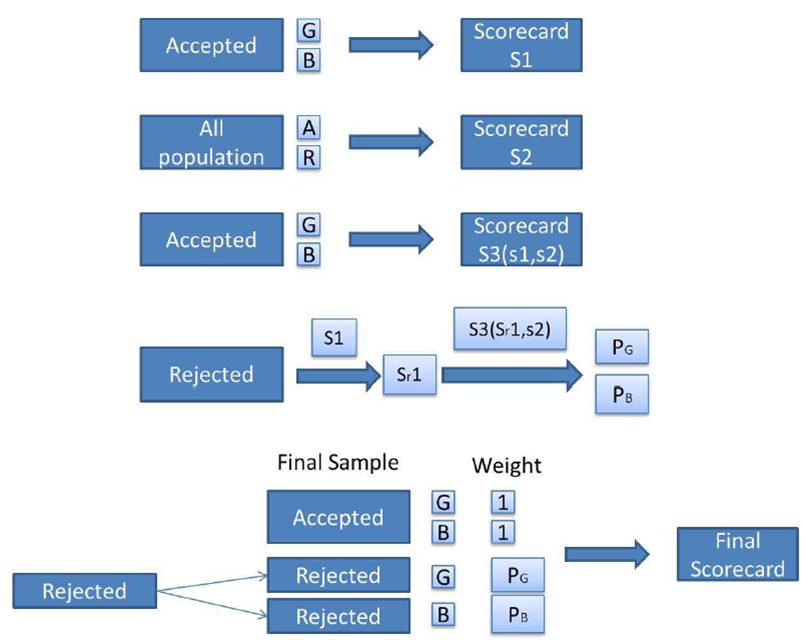
\includegraphics[width=0.5\textwidth]{figures/appendix/processusTwins.png}
\caption{The accompanying Figure of the Twins method in the internal documentation.}
\label{fig:twins}
\end{figure}

\begin{table}
\caption{\label{twins} Example of implementation of the Twins method on a small dataset}
{\setlength{\parindent}{0cm}
\begin{multicols}{4}

\begin{subfigure}[t]{0.22\textwidth}
\begin{center}
\begin{adjustbox}{max width=0.95\textwidth}
\begin{tabular}{l l l}
\toprule
\textbf{${\gls{bby}}$} & \textbf{${\gls{bbx}}$}\\
\midrule
1 & 0.562 \\
1 & 0.910 \\
0 & 0.430 \\
NA & 0.361 \\
NA & 0.402 \\
NA & 0.294 \\
\bottomrule
\end{tabular}
\end{adjustbox}
\end{center}

\caption{Development of scorecard $\hat{\gls{bth}}_\f$ on financed clients}
\label{twins:sfig1}
\end{subfigure}

\columnbreak

\begin{subfigure}[t]{0.22\textwidth}
\begin{center}
\begin{adjustbox}{max width=0.95\textwidth}
\begin{tabular}{l l l}
\toprule
\textbf{${\mathbf{z}}$} &  \textbf{${\gls{bbx}}$} \\
\midrule
\text{f} & 0.562 \\
\text{f} & 0.910 \\
\text{f} & 0.430 \\
\text{nf} & 0.361 \\
\text{nf} & 0.402 \\
\text{nf} & 0.294 \\
\bottomrule
\end{tabular}
\end{adjustbox}
\end{center}

\caption{Development of a scorecard $\hat{\gls{phi}}$ on all clients}
\label{twins:sfig2}
\end{subfigure}

\columnbreak

\begin{subfigure}[t]{0.22\textwidth}
\begin{center}
\begin{adjustbox}{max width=0.95\textwidth}
\begin{tabular}{l l l}
\toprule
\textbf{${\gls{bby}}$} & \textbf{$(1,\gls{bbx}_\f)' \hat{\gls{bth}}_\f$} & \textbf{$(1,\gls{bbx}_\f)' \hat{\gls{phi}}$}\\
\midrule
1 & 1.3 & 2.5\\
1 & 3.1 & 4.5 \\
0 & -0.3 & 0.4 \\
NA & -1.2 & -0.5 \\
NA & -0.4 & 0.3 \\
NA & -2.0 & -2.5 \\
\bottomrule
\end{tabular}
\end{adjustbox}
\end{center}

\caption{Development of a new scorecard on financed clients}
\label{twins:sfig3}
\end{subfigure}

\columnbreak

\begin{subfigure}[t]{0.22\textwidth}
\begin{center}
\begin{adjustbox}{max width=0.95\textwidth}
\begin{tabular}{l l l}
\toprule
\textbf{Weight} & \textbf{$\hat{\gls{bby}}_{\nf}$} & \textbf{${\gls{bbx}}_{\nf}$}\\
\midrule
1 & 1 & 0.562 \\
1 & 1 & 0.910 \\
1 & 0 & 0.430 \\
0.64 & 0 & 0.361 \\
0.73 & 0 & 0.402 \\
0.44 & 0 & 0.294 \\
0.36 & 1 & 0.361 \\
0.27 & 1 & 0.402 \\
0.37 & 1 & 0.294 \\
\bottomrule
\end{tabular}
\end{adjustbox}
\end{center}

\caption{Inference for not financed clients}
\label{twins:sfig4}
\end{subfigure}

\end{multicols}
}
\end{table}

Following notations introduced in Chapter~\ref{chap2}, we have:
\[ \ell(\gls{bth};(\bm{1},\gls{bbx}_{\f})' \hat{\gls{phi}}, (\bm{1},\gls{bbx}_{\f})' \hat{\gls{bth}}_\f, \gls{bby}_{\f}) = \sum_{i=1}^{n} \ln(p_{\gls{bth}}(y_i | (1, \gls{bx}_i)' \hat{\gls{bth}}_{\f}, (1, \gls{bx}_i)' \hat{\gls{phi}})).\]
We can rewrite $\ell(\gls{bth};(\bm{1},\gls{bbx}_{\f})' \hat{\gls{phi}}, (\bm{1},\gls{bbx}_{\f})' \hat{\gls{bth}}_\f, \gls{bby}_{\f})$ by remarking that the logit of $p_{\gls{bth}}(y_i | (1, \gls{bx}_i)' \hat{\gls{bth}}_{\f}, (1, \gls{bx}_i)' \hat{\gls{phi}})$ is a linear combination of $\gls{bx}$.
%: $\ell(\gls{bth};(\bm{1},\gls{bbx})' \hat{\gls{phi}}, (\bm{1},\gls{bbx})' \hat{\gls{bth}}_\f, \gls{bby}) = \ell(\theta;\gls{bbx}^{\text{f}}, \gls{bby}^{\text{f}})$ where $\begin{cases}
%\gls{bth} = (\theta_0,\theta_1,\theta_2). \\
%\theta_j = \delta_1 \hat{\theta}_{\text{f}j} + \delta_2 \hat{\zeta}_{j} \text{ for } 1 \leq j \leq d. \\
%\theta_0 = \delta_0 + \delta_1 \hat{\theta}_{\text{f}0} + \delta_2 \hat{\zeta}_{0}.
%\end{cases}$
We know that $\hat{\gls{bth}}_{\text{f}} \in \argmax_{\gls{bth} \in \Theta} \ell(\gls{bth};\gls{bbx}_{\text{f}},\gls{bby}_{\text{f}})$ so that under the identifiability assumption, this method will give the same results as $\hat{\gls{bth}}^{\text{f}}$. In terms of $\gls{KL}$ divergence and as for Fuzzy Augmentation, this method is useless because it is no different than the financed clients model.

\subsection{Parcelling} \label{Parceling}

Parcelling is a process of reweighing according to the probability of default by score-band that is adjusted by the credit modeler. It has been documented in \cite{saporta,banasik,RI6}, as well as in~\cite{groupe} where Figure~\ref{fig:parceling} is given.

\begin{enumerate}
\item Construct Scorecard ``Known Good Bad'' (KGB) $\hat{\gls{bth}}_\f$ with financed clients' data (Figure~\ref{parcel:sfig1});
\item Create $K$ score bands $B_1, \ldots, B_K$ according to $p_{\hat{\gls{bth}}_\f}(1 | \gls{bx})$;
\item Compute the observed default rate for each band $T(k) = \dfrac{|\text{Bad financed in } B_k|}{|B_k|}$, $1 \leq k  \leq K$;
\item Infer for each band the not financed default rate $U(k) = \epsilon_k T(k)$ where $1 < \epsilon_1 < \ldots < \epsilon_k < \ldots < \epsilon_K$ (Figure~\ref{parcel:sfig2});
\item Reintegrate 2 times each rejected applicant from $B_k$ with weight $U(k)$ as bad and weight $1-U(k)$ as good, like the Fuzzy Augmentation method in Section \ref{fuzzy} (Figure~\ref{parcel:sfig3});
\item Construct the final scorecard.
\end{enumerate}

\begin{figure}
\centering
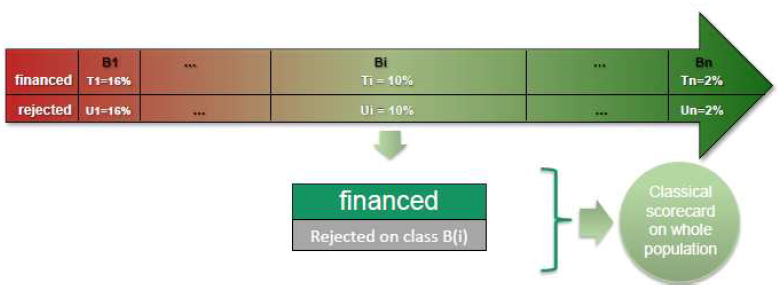
\includegraphics[width=0.5\textwidth]{figures/appendix/processusParcelling.png}
\caption{The accompanying Figure of the Parceling method in the internal documentation.}
\label{fig:parceling}
\end{figure}


\begin{table}
\caption{\label{parcel} Example of implementation of the Parcelling method on a small dataset}
{\setlength{\parindent}{0cm}
\begin{multicols}{3}

\begin{subfigure}[t]{0.31\textwidth}
\begin{center}
\begin{adjustbox}{max width=\textwidth}
\begin{tabular}{l l l}
\toprule
\textbf{Weight} & \textbf{${\gls{bby}}_{\f}$} & \textbf{${\gls{bbx}}_{\f}$}\\
\midrule
1 & 1 & 0.562 \\
1 & 1 & 0.910 \\
1 & 0 & 0.430 \\
\bottomrule
\end{tabular}
\end{adjustbox}
\end{center}

\caption{Development of scorecard $p_{\hat{\gls{bth}}_\f}(1 | \gls{bx})$ on financed clients}
\label{parcel:sfig1}
\end{subfigure}

\columnbreak

\begin{subfigure}[t]{0.31\textwidth}
\begin{center}
\begin{adjustbox}{max width=\textwidth}
\begin{tabular}{l l l}
\toprule
\textbf{Score-band} & \textbf{$T$} &  \textbf{$U$} \\
\midrule
1 & 0.5 & 0.8 \\
... & ... & ... \\
K & 0.01 & 0.04 \\
\bottomrule
\end{tabular}
\end{adjustbox}
\end{center}

\caption{Calculation of $T(k)$ and $U(k)$}
\label{parcel:sfig2}
\end{subfigure}

\columnbreak

\begin{subfigure}[t]{0.31\textwidth}
\begin{center}
\begin{adjustbox}{max width=\textwidth}
\begin{tabular}{l l l}
\toprule
\textbf{Weight} & \textbf{${\gls{bby}}$} & \textbf{${\gls{bbx}}$}\\
\midrule
1 & 0 & 0.562 \\
1 & 1 & 0.910 \\
1 & 0 & 0.430 \\
1 & 1 & 0.347 \\
1 & 0 & 0.140 \\
1 & 0 & 0.295 \\
\bottomrule
\end{tabular}
\end{adjustbox}
\end{center}

\caption{Inference for not financed clients}
\label{parcel:sfig3}
\end{subfigure}

\end{multicols}
}
\end{table}



\subsection{Simulation of reject inference methods applied to multivariate gaussian data} \label{subsec:app_reject_sim}

This early work aimed at comparing several reject inference methods in the well-specified model-case for 8 multivariate Gaussian features on Figure~\ref{fig:simu_4var} and 20 features on Figure~\ref{fig:simu_30var} in terms of error rate. The horizontal axis represents the cut-off value of a \gls{lr} that simulates the acceptance / rejection mechanism $p_{\gls{phi}}(\gls{z} | \gls{bx})$, such that it roughly corresponds to the fraction of missing labels $\gls{bby}_{\nf}$. In this setting, the semi-supervised generative approach obviously yields better results since the data lies in its restricted hypothesis space and it is able to use the predictors with missing labels $\gls{bbx}_{\nf}$. As explained thoroughly in Chapter~\ref{chap2}, standard \gls{lr} and Augmentation perform similarly (since they are both well-specified models and we are in a \gls{mar} setting). Parcelling does not work well since it is designed for a \gls{mnar} setting. In presence of well-separated data, Reclassification works well with 20 features since the true decision boundary is ``sharp'' (see the very small error rate) such that $\argmax_y \hat{p}(y | \gls{bx}) \approx \max_y \hat{p}(y | \gls{bx})$, which is less apparent with 8 features. In both cases, the mean of all features is $0$ (resp.\ $1$) if $Y=0$ (resp.\ $Y=1$) and the respective variance matrices are random positive definite matrices (see the Github repository of the manuscript at \url{https://www.github.com/adimajo/manuscrit_these} to reproduce them).

\begin{figure}[!ht]
\centering \resizebox{.8\textwidth}{!}{% Created by tikzDevice version 0.12 on 2019-07-02 15:28:50
% !TEX encoding = UTF-8 Unicode
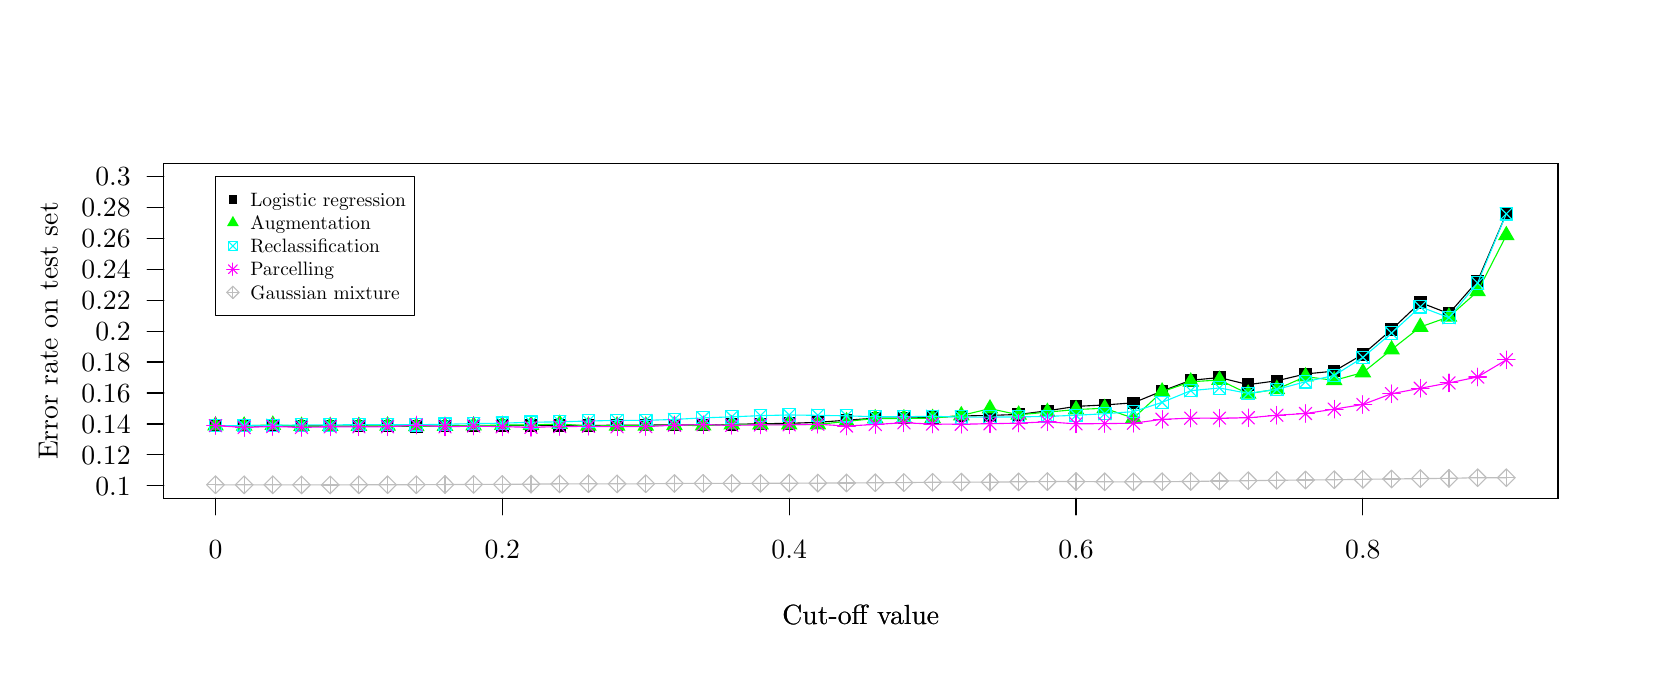
\begin{tikzpicture}[x=1pt,y=1pt]
\definecolor{fillColor}{RGB}{255,255,255}
\path[use as bounding box,fill=fillColor,fill opacity=0.00] (0,0) rectangle (578.16,231.26);
\begin{scope}
\path[clip] ( 49.20, 61.20) rectangle (552.96,182.06);
\definecolor{drawColor}{RGB}{0,0,0}

\path[draw=drawColor,line width= 0.4pt,line join=round,line cap=round] ( 67.86, 87.46) --
	( 78.22, 87.36) --
	( 88.59, 87.31) --
	( 98.95, 87.34) --
	(109.32, 87.29) --
	(119.68, 87.31) --
	(130.05, 87.29) --
	(140.42, 87.21) --
	(150.78, 87.31) --
	(161.15, 87.36) --
	(171.51, 87.47) --
	(181.88, 87.54) --
	(192.24, 87.54) --
	(202.61, 87.50) --
	(212.97, 87.62) --
	(223.34, 87.63) --
	(233.70, 87.75) --
	(244.07, 87.66) --
	(254.44, 87.89) --
	(264.80, 88.14) --
	(275.17, 88.28) --
	(285.53, 88.65) --
	(295.90, 89.42) --
	(306.26, 90.16) --
	(316.63, 90.18) --
	(326.99, 90.40) --
	(337.36, 90.94) --
	(347.72, 91.14) --
	(358.09, 91.50) --
	(368.46, 92.82) --
	(378.82, 94.41) --
	(389.19, 94.93) --
	(399.55, 95.70) --
	(409.92, 99.95) --
	(420.28,103.84) --
	(430.65,104.83) --
	(441.01,102.27) --
	(451.38,103.66) --
	(461.74,106.13) --
	(472.11,107.15) --
	(482.48,113.22) --
	(492.84,122.14) --
	(503.21,131.95) --
	(513.57,127.94) --
	(523.94,139.76) --
	(534.30,164.08);
\definecolor{fillColor}{RGB}{0,0,0}

\path[fill=fillColor] ( 65.61, 85.21) --
	( 70.11, 85.21) --
	( 70.11, 89.71) --
	( 65.61, 89.71) --
	cycle;

\path[fill=fillColor] ( 75.97, 85.11) --
	( 80.47, 85.11) --
	( 80.47, 89.61) --
	( 75.97, 89.61) --
	cycle;

\path[fill=fillColor] ( 86.34, 85.06) --
	( 90.84, 85.06) --
	( 90.84, 89.56) --
	( 86.34, 89.56) --
	cycle;

\path[fill=fillColor] ( 96.70, 85.09) --
	(101.20, 85.09) --
	(101.20, 89.59) --
	( 96.70, 89.59) --
	cycle;

\path[fill=fillColor] (107.07, 85.04) --
	(111.57, 85.04) --
	(111.57, 89.54) --
	(107.07, 89.54) --
	cycle;

\path[fill=fillColor] (117.43, 85.06) --
	(121.93, 85.06) --
	(121.93, 89.56) --
	(117.43, 89.56) --
	cycle;

\path[fill=fillColor] (127.80, 85.04) --
	(132.30, 85.04) --
	(132.30, 89.54) --
	(127.80, 89.54) --
	cycle;

\path[fill=fillColor] (138.17, 84.96) --
	(142.67, 84.96) --
	(142.67, 89.46) --
	(138.17, 89.46) --
	cycle;

\path[fill=fillColor] (148.53, 85.06) --
	(153.03, 85.06) --
	(153.03, 89.56) --
	(148.53, 89.56) --
	cycle;

\path[fill=fillColor] (158.90, 85.11) --
	(163.40, 85.11) --
	(163.40, 89.61) --
	(158.90, 89.61) --
	cycle;

\path[fill=fillColor] (169.26, 85.22) --
	(173.76, 85.22) --
	(173.76, 89.72) --
	(169.26, 89.72) --
	cycle;

\path[fill=fillColor] (179.63, 85.29) --
	(184.13, 85.29) --
	(184.13, 89.79) --
	(179.63, 89.79) --
	cycle;

\path[fill=fillColor] (189.99, 85.29) --
	(194.49, 85.29) --
	(194.49, 89.79) --
	(189.99, 89.79) --
	cycle;

\path[fill=fillColor] (200.36, 85.25) --
	(204.86, 85.25) --
	(204.86, 89.75) --
	(200.36, 89.75) --
	cycle;

\path[fill=fillColor] (210.72, 85.37) --
	(215.22, 85.37) --
	(215.22, 89.87) --
	(210.72, 89.87) --
	cycle;

\path[fill=fillColor] (221.09, 85.38) --
	(225.59, 85.38) --
	(225.59, 89.88) --
	(221.09, 89.88) --
	cycle;

\path[fill=fillColor] (231.45, 85.50) --
	(235.95, 85.50) --
	(235.95, 90.00) --
	(231.45, 90.00) --
	cycle;

\path[fill=fillColor] (241.82, 85.41) --
	(246.32, 85.41) --
	(246.32, 89.91) --
	(241.82, 89.91) --
	cycle;

\path[fill=fillColor] (252.19, 85.64) --
	(256.69, 85.64) --
	(256.69, 90.14) --
	(252.19, 90.14) --
	cycle;

\path[fill=fillColor] (262.55, 85.89) --
	(267.05, 85.89) --
	(267.05, 90.39) --
	(262.55, 90.39) --
	cycle;

\path[fill=fillColor] (272.92, 86.03) --
	(277.42, 86.03) --
	(277.42, 90.53) --
	(272.92, 90.53) --
	cycle;

\path[fill=fillColor] (283.28, 86.40) --
	(287.78, 86.40) --
	(287.78, 90.90) --
	(283.28, 90.90) --
	cycle;

\path[fill=fillColor] (293.65, 87.17) --
	(298.15, 87.17) --
	(298.15, 91.67) --
	(293.65, 91.67) --
	cycle;

\path[fill=fillColor] (304.01, 87.91) --
	(308.51, 87.91) --
	(308.51, 92.41) --
	(304.01, 92.41) --
	cycle;

\path[fill=fillColor] (314.38, 87.93) --
	(318.88, 87.93) --
	(318.88, 92.43) --
	(314.38, 92.43) --
	cycle;

\path[fill=fillColor] (324.74, 88.15) --
	(329.24, 88.15) --
	(329.24, 92.65) --
	(324.74, 92.65) --
	cycle;

\path[fill=fillColor] (335.11, 88.69) --
	(339.61, 88.69) --
	(339.61, 93.19) --
	(335.11, 93.19) --
	cycle;

\path[fill=fillColor] (345.47, 88.89) --
	(349.97, 88.89) --
	(349.97, 93.39) --
	(345.47, 93.39) --
	cycle;

\path[fill=fillColor] (355.84, 89.25) --
	(360.34, 89.25) --
	(360.34, 93.75) --
	(355.84, 93.75) --
	cycle;

\path[fill=fillColor] (366.21, 90.57) --
	(370.71, 90.57) --
	(370.71, 95.07) --
	(366.21, 95.07) --
	cycle;

\path[fill=fillColor] (376.57, 92.16) --
	(381.07, 92.16) --
	(381.07, 96.66) --
	(376.57, 96.66) --
	cycle;

\path[fill=fillColor] (386.94, 92.68) --
	(391.44, 92.68) --
	(391.44, 97.18) --
	(386.94, 97.18) --
	cycle;

\path[fill=fillColor] (397.30, 93.45) --
	(401.80, 93.45) --
	(401.80, 97.95) --
	(397.30, 97.95) --
	cycle;

\path[fill=fillColor] (407.67, 97.70) --
	(412.17, 97.70) --
	(412.17,102.20) --
	(407.67,102.20) --
	cycle;

\path[fill=fillColor] (418.03,101.59) --
	(422.53,101.59) --
	(422.53,106.09) --
	(418.03,106.09) --
	cycle;

\path[fill=fillColor] (428.40,102.58) --
	(432.90,102.58) --
	(432.90,107.08) --
	(428.40,107.08) --
	cycle;

\path[fill=fillColor] (438.76,100.02) --
	(443.26,100.02) --
	(443.26,104.52) --
	(438.76,104.52) --
	cycle;

\path[fill=fillColor] (449.13,101.41) --
	(453.63,101.41) --
	(453.63,105.91) --
	(449.13,105.91) --
	cycle;

\path[fill=fillColor] (459.49,103.88) --
	(463.99,103.88) --
	(463.99,108.38) --
	(459.49,108.38) --
	cycle;

\path[fill=fillColor] (469.86,104.90) --
	(474.36,104.90) --
	(474.36,109.40) --
	(469.86,109.40) --
	cycle;

\path[fill=fillColor] (480.23,110.97) --
	(484.73,110.97) --
	(484.73,115.47) --
	(480.23,115.47) --
	cycle;

\path[fill=fillColor] (490.59,119.89) --
	(495.09,119.89) --
	(495.09,124.39) --
	(490.59,124.39) --
	cycle;

\path[fill=fillColor] (500.96,129.70) --
	(505.46,129.70) --
	(505.46,134.20) --
	(500.96,134.20) --
	cycle;

\path[fill=fillColor] (511.32,125.69) --
	(515.82,125.69) --
	(515.82,130.19) --
	(511.32,130.19) --
	cycle;

\path[fill=fillColor] (521.69,137.51) --
	(526.19,137.51) --
	(526.19,142.01) --
	(521.69,142.01) --
	cycle;

\path[fill=fillColor] (532.05,161.83) --
	(536.55,161.83) --
	(536.55,166.33) --
	(532.05,166.33) --
	cycle;
\end{scope}
\begin{scope}
\path[clip] (  0.00,  0.00) rectangle (578.16,231.26);
\definecolor{drawColor}{RGB}{0,0,0}

\path[draw=drawColor,line width= 0.4pt,line join=round,line cap=round] ( 49.20, 61.20) --
	(552.96, 61.20) --
	(552.96,182.06) --
	( 49.20,182.06) --
	( 49.20, 61.20);
\end{scope}
\begin{scope}
\path[clip] (  0.00,  0.00) rectangle (578.16,231.26);
\definecolor{drawColor}{RGB}{0,0,0}

\node[text=drawColor,anchor=base,inner sep=0pt, outer sep=0pt, scale=  1.00] at (301.08, 15.60) {Cut-off value};

\node[text=drawColor,rotate= 90.00,anchor=base,inner sep=0pt, outer sep=0pt, scale=  1.00] at ( 10.80,121.63) {Error rate on test set};
\end{scope}
\begin{scope}
\path[clip] ( 49.20, 61.20) rectangle (552.96,182.06);
\definecolor{drawColor}{RGB}{0,255,0}

\path[draw=drawColor,line width= 0.4pt,line join=round,line cap=round] ( 67.86, 87.46) --
	( 78.22, 87.40) --
	( 88.59, 87.71) --
	( 98.95, 87.30) --
	(109.32, 87.27) --
	(119.68, 87.30) --
	(130.05, 87.43) --
	(140.42, 87.19) --
	(150.78, 87.33) --
	(161.15, 87.46) --
	(171.51, 87.66) --
	(181.88, 87.68) --
	(192.24, 88.04) --
	(202.61, 87.36) --
	(212.97, 87.44) --
	(223.34, 87.40) --
	(233.70, 87.61) --
	(244.07, 87.47) --
	(254.44, 87.86) --
	(264.80, 87.88) --
	(275.17, 87.81) --
	(285.53, 87.88) --
	(295.90, 88.98) --
	(306.26, 90.05) --
	(316.63, 90.05) --
	(326.99, 90.15) --
	(337.36, 91.14) --
	(347.72, 93.59) --
	(358.09, 91.37) --
	(368.46, 92.33) --
	(378.82, 93.27) --
	(389.19, 93.74) --
	(399.55, 90.13) --
	(409.92, 99.71) --
	(420.28,103.31) --
	(430.65,103.94) --
	(441.01, 98.98) --
	(451.38,100.63) --
	(461.74,105.16) --
	(472.11,103.82) --
	(482.48,106.63) --
	(492.84,114.95) --
	(503.21,123.09) --
	(513.57,126.77) --
	(523.94,135.96) --
	(534.30,156.20);
\definecolor{fillColor}{RGB}{0,255,0}

\path[fill=fillColor] ( 67.86, 90.96) --
	( 70.89, 85.71) --
	( 64.83, 85.71) --
	cycle;

\path[fill=fillColor] ( 78.22, 90.90) --
	( 81.25, 85.65) --
	( 75.19, 85.65) --
	cycle;

\path[fill=fillColor] ( 88.59, 91.21) --
	( 91.62, 85.96) --
	( 85.56, 85.96) --
	cycle;

\path[fill=fillColor] ( 98.95, 90.80) --
	(101.98, 85.55) --
	( 95.92, 85.55) --
	cycle;

\path[fill=fillColor] (109.32, 90.77) --
	(112.35, 85.52) --
	(106.29, 85.52) --
	cycle;

\path[fill=fillColor] (119.68, 90.80) --
	(122.72, 85.55) --
	(116.65, 85.55) --
	cycle;

\path[fill=fillColor] (130.05, 90.93) --
	(133.08, 85.68) --
	(127.02, 85.68) --
	cycle;

\path[fill=fillColor] (140.42, 90.68) --
	(143.45, 85.44) --
	(137.39, 85.44) --
	cycle;

\path[fill=fillColor] (150.78, 90.83) --
	(153.81, 85.58) --
	(147.75, 85.58) --
	cycle;

\path[fill=fillColor] (161.15, 90.96) --
	(164.18, 85.71) --
	(158.12, 85.71) --
	cycle;

\path[fill=fillColor] (171.51, 91.15) --
	(174.54, 85.91) --
	(168.48, 85.91) --
	cycle;

\path[fill=fillColor] (181.88, 91.18) --
	(184.91, 85.93) --
	(178.85, 85.93) --
	cycle;

\path[fill=fillColor] (192.24, 91.54) --
	(195.27, 86.29) --
	(189.21, 86.29) --
	cycle;

\path[fill=fillColor] (202.61, 90.86) --
	(205.64, 85.61) --
	(199.58, 85.61) --
	cycle;

\path[fill=fillColor] (212.97, 90.94) --
	(216.00, 85.69) --
	(209.94, 85.69) --
	cycle;

\path[fill=fillColor] (223.34, 90.90) --
	(226.37, 85.65) --
	(220.31, 85.65) --
	cycle;

\path[fill=fillColor] (233.70, 91.11) --
	(236.73, 85.86) --
	(230.67, 85.86) --
	cycle;

\path[fill=fillColor] (244.07, 90.97) --
	(247.10, 85.72) --
	(241.04, 85.72) --
	cycle;

\path[fill=fillColor] (254.44, 91.36) --
	(257.47, 86.11) --
	(251.41, 86.11) --
	cycle;

\path[fill=fillColor] (264.80, 91.38) --
	(267.83, 86.13) --
	(261.77, 86.13) --
	cycle;

\path[fill=fillColor] (275.17, 91.31) --
	(278.20, 86.06) --
	(272.14, 86.06) --
	cycle;

\path[fill=fillColor] (285.53, 91.38) --
	(288.56, 86.13) --
	(282.50, 86.13) --
	cycle;

\path[fill=fillColor] (295.90, 92.48) --
	(298.93, 87.23) --
	(292.87, 87.23) --
	cycle;

\path[fill=fillColor] (306.26, 93.54) --
	(309.29, 88.30) --
	(303.23, 88.30) --
	cycle;

\path[fill=fillColor] (316.63, 93.54) --
	(319.66, 88.30) --
	(313.60, 88.30) --
	cycle;

\path[fill=fillColor] (326.99, 93.64) --
	(330.02, 88.40) --
	(323.96, 88.40) --
	cycle;

\path[fill=fillColor] (337.36, 94.64) --
	(340.39, 89.39) --
	(334.33, 89.39) --
	cycle;

\path[fill=fillColor] (347.72, 97.09) --
	(350.75, 91.84) --
	(344.69, 91.84) --
	cycle;

\path[fill=fillColor] (358.09, 94.87) --
	(361.12, 89.62) --
	(355.06, 89.62) --
	cycle;

\path[fill=fillColor] (368.46, 95.83) --
	(371.49, 90.58) --
	(365.43, 90.58) --
	cycle;

\path[fill=fillColor] (378.82, 96.77) --
	(381.85, 91.52) --
	(375.79, 91.52) --
	cycle;

\path[fill=fillColor] (389.19, 97.24) --
	(392.22, 91.99) --
	(386.16, 91.99) --
	cycle;

\path[fill=fillColor] (399.55, 93.63) --
	(402.58, 88.39) --
	(396.52, 88.39) --
	cycle;

\path[fill=fillColor] (409.92,103.21) --
	(412.95, 97.96) --
	(406.89, 97.96) --
	cycle;

\path[fill=fillColor] (420.28,106.81) --
	(423.31,101.56) --
	(417.25,101.56) --
	cycle;

\path[fill=fillColor] (430.65,107.44) --
	(433.68,102.19) --
	(427.62,102.19) --
	cycle;

\path[fill=fillColor] (441.01,102.47) --
	(444.04, 97.23) --
	(437.98, 97.23) --
	cycle;

\path[fill=fillColor] (451.38,104.13) --
	(454.41, 98.88) --
	(448.35, 98.88) --
	cycle;

\path[fill=fillColor] (461.74,108.66) --
	(464.77,103.41) --
	(458.71,103.41) --
	cycle;

\path[fill=fillColor] (472.11,107.31) --
	(475.14,102.07) --
	(469.08,102.07) --
	cycle;

\path[fill=fillColor] (482.48,110.13) --
	(485.51,104.88) --
	(479.44,104.88) --
	cycle;

\path[fill=fillColor] (492.84,118.44) --
	(495.87,113.20) --
	(489.81,113.20) --
	cycle;

\path[fill=fillColor] (503.21,126.59) --
	(506.24,121.34) --
	(500.18,121.34) --
	cycle;

\path[fill=fillColor] (513.57,130.27) --
	(516.60,125.02) --
	(510.54,125.02) --
	cycle;

\path[fill=fillColor] (523.94,139.46) --
	(526.97,134.21) --
	(520.91,134.21) --
	cycle;

\path[fill=fillColor] (534.30,159.69) --
	(537.33,154.45) --
	(531.27,154.45) --
	cycle;
\end{scope}
\begin{scope}
\path[clip] (  0.00,  0.00) rectangle (578.16,231.26);
\definecolor{drawColor}{RGB}{0,0,0}

\path[draw=drawColor,line width= 0.4pt,line join=round,line cap=round] ( 49.20, 61.20) --
	(552.96, 61.20) --
	(552.96,182.06) --
	( 49.20,182.06) --
	( 49.20, 61.20);
\end{scope}
\begin{scope}
\path[clip] (  0.00,  0.00) rectangle (578.16,231.26);
\definecolor{drawColor}{RGB}{0,0,0}

%\node[text=drawColor,anchor=base,inner sep=0pt, outer sep=0pt, scale=  1.00] at (301.08, 15.60) {Cut-off value};

%\node[text=drawColor,rotate= 90.00,anchor=base,inner sep=0pt, outer sep=0pt, scale=  1.00] at ( 10.80,121.63) {Error rate on test set};
\end{scope}
\begin{scope}
\path[clip] ( 49.20, 61.20) rectangle (552.96,182.06);
\definecolor{drawColor}{RGB}{0,255,255}

\path[draw=drawColor,line width= 0.4pt,line join=round,line cap=round] ( 67.86, 87.46) --
	( 78.22, 87.46) --
	( 88.59, 87.57) --
	( 98.95, 87.71) --
	(109.32, 87.72) --
	(119.68, 87.80) --
	(130.05, 87.80) --
	(140.42, 87.77) --
	(150.78, 87.95) --
	(161.15, 88.18) --
	(171.51, 88.34) --
	(181.88, 88.68) --
	(192.24, 88.83) --
	(202.61, 89.13) --
	(212.97, 89.35) --
	(223.34, 89.35) --
	(233.70, 89.70) --
	(244.07, 90.26) --
	(254.44, 90.63) --
	(264.80, 91.07) --
	(275.17, 91.31) --
	(285.53, 91.17) --
	(295.90, 91.00) --
	(306.26, 90.67) --
	(316.63, 90.68) --
	(326.99, 90.83) --
	(337.36, 90.55) --
	(347.72, 90.55) --
	(358.09, 90.60) --
	(368.46, 90.80) --
	(378.82, 91.19) --
	(389.19, 91.77) --
	(399.55, 92.50) --
	(409.92, 95.86) --
	(420.28,100.09) --
	(430.65,101.06) --
	(441.01, 99.12) --
	(451.38,100.54) --
	(461.74,103.32) --
	(472.11,105.58) --
	(482.48,112.11) --
	(492.84,120.89) --
	(503.21,130.41) --
	(513.57,126.47) --
	(523.94,139.00) --
	(534.30,164.00);

\path[draw=drawColor,line width= 0.4pt,line join=round,line cap=round] ( 65.61, 85.21) rectangle ( 70.11, 89.71);

\path[draw=drawColor,line width= 0.4pt,line join=round,line cap=round] ( 65.61, 85.21) -- ( 70.11, 89.71);

\path[draw=drawColor,line width= 0.4pt,line join=round,line cap=round] ( 65.61, 89.71) -- ( 70.11, 85.21);

\path[draw=drawColor,line width= 0.4pt,line join=round,line cap=round] ( 75.97, 85.21) rectangle ( 80.47, 89.71);

\path[draw=drawColor,line width= 0.4pt,line join=round,line cap=round] ( 75.97, 85.21) -- ( 80.47, 89.71);

\path[draw=drawColor,line width= 0.4pt,line join=round,line cap=round] ( 75.97, 89.71) -- ( 80.47, 85.21);

\path[draw=drawColor,line width= 0.4pt,line join=round,line cap=round] ( 86.34, 85.32) rectangle ( 90.84, 89.82);

\path[draw=drawColor,line width= 0.4pt,line join=round,line cap=round] ( 86.34, 85.32) -- ( 90.84, 89.82);

\path[draw=drawColor,line width= 0.4pt,line join=round,line cap=round] ( 86.34, 89.82) -- ( 90.84, 85.32);

\path[draw=drawColor,line width= 0.4pt,line join=round,line cap=round] ( 96.70, 85.46) rectangle (101.20, 89.96);

\path[draw=drawColor,line width= 0.4pt,line join=round,line cap=round] ( 96.70, 85.46) -- (101.20, 89.96);

\path[draw=drawColor,line width= 0.4pt,line join=round,line cap=round] ( 96.70, 89.96) -- (101.20, 85.46);

\path[draw=drawColor,line width= 0.4pt,line join=round,line cap=round] (107.07, 85.47) rectangle (111.57, 89.97);

\path[draw=drawColor,line width= 0.4pt,line join=round,line cap=round] (107.07, 85.47) -- (111.57, 89.97);

\path[draw=drawColor,line width= 0.4pt,line join=round,line cap=round] (107.07, 89.97) -- (111.57, 85.47);

\path[draw=drawColor,line width= 0.4pt,line join=round,line cap=round] (117.43, 85.55) rectangle (121.93, 90.05);

\path[draw=drawColor,line width= 0.4pt,line join=round,line cap=round] (117.43, 85.55) -- (121.93, 90.05);

\path[draw=drawColor,line width= 0.4pt,line join=round,line cap=round] (117.43, 90.05) -- (121.93, 85.55);

\path[draw=drawColor,line width= 0.4pt,line join=round,line cap=round] (127.80, 85.55) rectangle (132.30, 90.05);

\path[draw=drawColor,line width= 0.4pt,line join=round,line cap=round] (127.80, 85.55) -- (132.30, 90.05);

\path[draw=drawColor,line width= 0.4pt,line join=round,line cap=round] (127.80, 90.05) -- (132.30, 85.55);

\path[draw=drawColor,line width= 0.4pt,line join=round,line cap=round] (138.17, 85.52) rectangle (142.67, 90.02);

\path[draw=drawColor,line width= 0.4pt,line join=round,line cap=round] (138.17, 85.52) -- (142.67, 90.02);

\path[draw=drawColor,line width= 0.4pt,line join=round,line cap=round] (138.17, 90.02) -- (142.67, 85.52);

\path[draw=drawColor,line width= 0.4pt,line join=round,line cap=round] (148.53, 85.70) rectangle (153.03, 90.20);

\path[draw=drawColor,line width= 0.4pt,line join=round,line cap=round] (148.53, 85.70) -- (153.03, 90.20);

\path[draw=drawColor,line width= 0.4pt,line join=round,line cap=round] (148.53, 90.20) -- (153.03, 85.70);

\path[draw=drawColor,line width= 0.4pt,line join=round,line cap=round] (158.90, 85.93) rectangle (163.40, 90.43);

\path[draw=drawColor,line width= 0.4pt,line join=round,line cap=round] (158.90, 85.93) -- (163.40, 90.43);

\path[draw=drawColor,line width= 0.4pt,line join=round,line cap=round] (158.90, 90.43) -- (163.40, 85.93);

\path[draw=drawColor,line width= 0.4pt,line join=round,line cap=round] (169.26, 86.09) rectangle (173.76, 90.59);

\path[draw=drawColor,line width= 0.4pt,line join=round,line cap=round] (169.26, 86.09) -- (173.76, 90.59);

\path[draw=drawColor,line width= 0.4pt,line join=round,line cap=round] (169.26, 90.59) -- (173.76, 86.09);

\path[draw=drawColor,line width= 0.4pt,line join=round,line cap=round] (179.63, 86.43) rectangle (184.13, 90.93);

\path[draw=drawColor,line width= 0.4pt,line join=round,line cap=round] (179.63, 86.43) -- (184.13, 90.93);

\path[draw=drawColor,line width= 0.4pt,line join=round,line cap=round] (179.63, 90.93) -- (184.13, 86.43);

\path[draw=drawColor,line width= 0.4pt,line join=round,line cap=round] (189.99, 86.58) rectangle (194.49, 91.08);

\path[draw=drawColor,line width= 0.4pt,line join=round,line cap=round] (189.99, 86.58) -- (194.49, 91.08);

\path[draw=drawColor,line width= 0.4pt,line join=round,line cap=round] (189.99, 91.08) -- (194.49, 86.58);

\path[draw=drawColor,line width= 0.4pt,line join=round,line cap=round] (200.36, 86.88) rectangle (204.86, 91.38);

\path[draw=drawColor,line width= 0.4pt,line join=round,line cap=round] (200.36, 86.88) -- (204.86, 91.38);

\path[draw=drawColor,line width= 0.4pt,line join=round,line cap=round] (200.36, 91.38) -- (204.86, 86.88);

\path[draw=drawColor,line width= 0.4pt,line join=round,line cap=round] (210.72, 87.10) rectangle (215.22, 91.60);

\path[draw=drawColor,line width= 0.4pt,line join=round,line cap=round] (210.72, 87.10) -- (215.22, 91.60);

\path[draw=drawColor,line width= 0.4pt,line join=round,line cap=round] (210.72, 91.60) -- (215.22, 87.10);

\path[draw=drawColor,line width= 0.4pt,line join=round,line cap=round] (221.09, 87.10) rectangle (225.59, 91.60);

\path[draw=drawColor,line width= 0.4pt,line join=round,line cap=round] (221.09, 87.10) -- (225.59, 91.60);

\path[draw=drawColor,line width= 0.4pt,line join=round,line cap=round] (221.09, 91.60) -- (225.59, 87.10);

\path[draw=drawColor,line width= 0.4pt,line join=round,line cap=round] (231.45, 87.45) rectangle (235.95, 91.95);

\path[draw=drawColor,line width= 0.4pt,line join=round,line cap=round] (231.45, 87.45) -- (235.95, 91.95);

\path[draw=drawColor,line width= 0.4pt,line join=round,line cap=round] (231.45, 91.95) -- (235.95, 87.45);

\path[draw=drawColor,line width= 0.4pt,line join=round,line cap=round] (241.82, 88.01) rectangle (246.32, 92.51);

\path[draw=drawColor,line width= 0.4pt,line join=round,line cap=round] (241.82, 88.01) -- (246.32, 92.51);

\path[draw=drawColor,line width= 0.4pt,line join=round,line cap=round] (241.82, 92.51) -- (246.32, 88.01);

\path[draw=drawColor,line width= 0.4pt,line join=round,line cap=round] (252.19, 88.38) rectangle (256.69, 92.88);

\path[draw=drawColor,line width= 0.4pt,line join=round,line cap=round] (252.19, 88.38) -- (256.69, 92.88);

\path[draw=drawColor,line width= 0.4pt,line join=round,line cap=round] (252.19, 92.88) -- (256.69, 88.38);

\path[draw=drawColor,line width= 0.4pt,line join=round,line cap=round] (262.55, 88.82) rectangle (267.05, 93.32);

\path[draw=drawColor,line width= 0.4pt,line join=round,line cap=round] (262.55, 88.82) -- (267.05, 93.32);

\path[draw=drawColor,line width= 0.4pt,line join=round,line cap=round] (262.55, 93.32) -- (267.05, 88.82);

\path[draw=drawColor,line width= 0.4pt,line join=round,line cap=round] (272.92, 89.06) rectangle (277.42, 93.56);

\path[draw=drawColor,line width= 0.4pt,line join=round,line cap=round] (272.92, 89.06) -- (277.42, 93.56);

\path[draw=drawColor,line width= 0.4pt,line join=round,line cap=round] (272.92, 93.56) -- (277.42, 89.06);

\path[draw=drawColor,line width= 0.4pt,line join=round,line cap=round] (283.28, 88.92) rectangle (287.78, 93.42);

\path[draw=drawColor,line width= 0.4pt,line join=round,line cap=round] (283.28, 88.92) -- (287.78, 93.42);

\path[draw=drawColor,line width= 0.4pt,line join=round,line cap=round] (283.28, 93.42) -- (287.78, 88.92);

\path[draw=drawColor,line width= 0.4pt,line join=round,line cap=round] (293.65, 88.75) rectangle (298.15, 93.25);

\path[draw=drawColor,line width= 0.4pt,line join=round,line cap=round] (293.65, 88.75) -- (298.15, 93.25);

\path[draw=drawColor,line width= 0.4pt,line join=round,line cap=round] (293.65, 93.25) -- (298.15, 88.75);

\path[draw=drawColor,line width= 0.4pt,line join=round,line cap=round] (304.01, 88.42) rectangle (308.51, 92.92);

\path[draw=drawColor,line width= 0.4pt,line join=round,line cap=round] (304.01, 88.42) -- (308.51, 92.92);

\path[draw=drawColor,line width= 0.4pt,line join=round,line cap=round] (304.01, 92.92) -- (308.51, 88.42);

\path[draw=drawColor,line width= 0.4pt,line join=round,line cap=round] (314.38, 88.43) rectangle (318.88, 92.93);

\path[draw=drawColor,line width= 0.4pt,line join=round,line cap=round] (314.38, 88.43) -- (318.88, 92.93);

\path[draw=drawColor,line width= 0.4pt,line join=round,line cap=round] (314.38, 92.93) -- (318.88, 88.43);

\path[draw=drawColor,line width= 0.4pt,line join=round,line cap=round] (324.74, 88.58) rectangle (329.24, 93.08);

\path[draw=drawColor,line width= 0.4pt,line join=round,line cap=round] (324.74, 88.58) -- (329.24, 93.08);

\path[draw=drawColor,line width= 0.4pt,line join=round,line cap=round] (324.74, 93.08) -- (329.24, 88.58);

\path[draw=drawColor,line width= 0.4pt,line join=round,line cap=round] (335.11, 88.30) rectangle (339.61, 92.80);

\path[draw=drawColor,line width= 0.4pt,line join=round,line cap=round] (335.11, 88.30) -- (339.61, 92.80);

\path[draw=drawColor,line width= 0.4pt,line join=round,line cap=round] (335.11, 92.80) -- (339.61, 88.30);

\path[draw=drawColor,line width= 0.4pt,line join=round,line cap=round] (345.47, 88.30) rectangle (349.97, 92.80);

\path[draw=drawColor,line width= 0.4pt,line join=round,line cap=round] (345.47, 88.30) -- (349.97, 92.80);

\path[draw=drawColor,line width= 0.4pt,line join=round,line cap=round] (345.47, 92.80) -- (349.97, 88.30);

\path[draw=drawColor,line width= 0.4pt,line join=round,line cap=round] (355.84, 88.35) rectangle (360.34, 92.85);

\path[draw=drawColor,line width= 0.4pt,line join=round,line cap=round] (355.84, 88.35) -- (360.34, 92.85);

\path[draw=drawColor,line width= 0.4pt,line join=round,line cap=round] (355.84, 92.85) -- (360.34, 88.35);

\path[draw=drawColor,line width= 0.4pt,line join=round,line cap=round] (366.21, 88.55) rectangle (370.71, 93.05);

\path[draw=drawColor,line width= 0.4pt,line join=round,line cap=round] (366.21, 88.55) -- (370.71, 93.05);

\path[draw=drawColor,line width= 0.4pt,line join=round,line cap=round] (366.21, 93.05) -- (370.71, 88.55);

\path[draw=drawColor,line width= 0.4pt,line join=round,line cap=round] (376.57, 88.94) rectangle (381.07, 93.44);

\path[draw=drawColor,line width= 0.4pt,line join=round,line cap=round] (376.57, 88.94) -- (381.07, 93.44);

\path[draw=drawColor,line width= 0.4pt,line join=round,line cap=round] (376.57, 93.44) -- (381.07, 88.94);

\path[draw=drawColor,line width= 0.4pt,line join=round,line cap=round] (386.94, 89.52) rectangle (391.44, 94.02);

\path[draw=drawColor,line width= 0.4pt,line join=round,line cap=round] (386.94, 89.52) -- (391.44, 94.02);

\path[draw=drawColor,line width= 0.4pt,line join=round,line cap=round] (386.94, 94.02) -- (391.44, 89.52);

\path[draw=drawColor,line width= 0.4pt,line join=round,line cap=round] (397.30, 90.25) rectangle (401.80, 94.75);

\path[draw=drawColor,line width= 0.4pt,line join=round,line cap=round] (397.30, 90.25) -- (401.80, 94.75);

\path[draw=drawColor,line width= 0.4pt,line join=round,line cap=round] (397.30, 94.75) -- (401.80, 90.25);

\path[draw=drawColor,line width= 0.4pt,line join=round,line cap=round] (407.67, 93.61) rectangle (412.17, 98.11);

\path[draw=drawColor,line width= 0.4pt,line join=round,line cap=round] (407.67, 93.61) -- (412.17, 98.11);

\path[draw=drawColor,line width= 0.4pt,line join=round,line cap=round] (407.67, 98.11) -- (412.17, 93.61);

\path[draw=drawColor,line width= 0.4pt,line join=round,line cap=round] (418.03, 97.84) rectangle (422.53,102.34);

\path[draw=drawColor,line width= 0.4pt,line join=round,line cap=round] (418.03, 97.84) -- (422.53,102.34);

\path[draw=drawColor,line width= 0.4pt,line join=round,line cap=round] (418.03,102.34) -- (422.53, 97.84);

\path[draw=drawColor,line width= 0.4pt,line join=round,line cap=round] (428.40, 98.81) rectangle (432.90,103.31);

\path[draw=drawColor,line width= 0.4pt,line join=round,line cap=round] (428.40, 98.81) -- (432.90,103.31);

\path[draw=drawColor,line width= 0.4pt,line join=round,line cap=round] (428.40,103.31) -- (432.90, 98.81);

\path[draw=drawColor,line width= 0.4pt,line join=round,line cap=round] (438.76, 96.87) rectangle (443.26,101.37);

\path[draw=drawColor,line width= 0.4pt,line join=round,line cap=round] (438.76, 96.87) -- (443.26,101.37);

\path[draw=drawColor,line width= 0.4pt,line join=round,line cap=round] (438.76,101.37) -- (443.26, 96.87);

\path[draw=drawColor,line width= 0.4pt,line join=round,line cap=round] (449.13, 98.29) rectangle (453.63,102.79);

\path[draw=drawColor,line width= 0.4pt,line join=round,line cap=round] (449.13, 98.29) -- (453.63,102.79);

\path[draw=drawColor,line width= 0.4pt,line join=round,line cap=round] (449.13,102.79) -- (453.63, 98.29);

\path[draw=drawColor,line width= 0.4pt,line join=round,line cap=round] (459.49,101.07) rectangle (463.99,105.57);

\path[draw=drawColor,line width= 0.4pt,line join=round,line cap=round] (459.49,101.07) -- (463.99,105.57);

\path[draw=drawColor,line width= 0.4pt,line join=round,line cap=round] (459.49,105.57) -- (463.99,101.07);

\path[draw=drawColor,line width= 0.4pt,line join=round,line cap=round] (469.86,103.33) rectangle (474.36,107.83);

\path[draw=drawColor,line width= 0.4pt,line join=round,line cap=round] (469.86,103.33) -- (474.36,107.83);

\path[draw=drawColor,line width= 0.4pt,line join=round,line cap=round] (469.86,107.83) -- (474.36,103.33);

\path[draw=drawColor,line width= 0.4pt,line join=round,line cap=round] (480.23,109.86) rectangle (484.73,114.36);

\path[draw=drawColor,line width= 0.4pt,line join=round,line cap=round] (480.23,109.86) -- (484.73,114.36);

\path[draw=drawColor,line width= 0.4pt,line join=round,line cap=round] (480.23,114.36) -- (484.73,109.86);

\path[draw=drawColor,line width= 0.4pt,line join=round,line cap=round] (490.59,118.64) rectangle (495.09,123.14);

\path[draw=drawColor,line width= 0.4pt,line join=round,line cap=round] (490.59,118.64) -- (495.09,123.14);

\path[draw=drawColor,line width= 0.4pt,line join=round,line cap=round] (490.59,123.14) -- (495.09,118.64);

\path[draw=drawColor,line width= 0.4pt,line join=round,line cap=round] (500.96,128.16) rectangle (505.46,132.66);

\path[draw=drawColor,line width= 0.4pt,line join=round,line cap=round] (500.96,128.16) -- (505.46,132.66);

\path[draw=drawColor,line width= 0.4pt,line join=round,line cap=round] (500.96,132.66) -- (505.46,128.16);

\path[draw=drawColor,line width= 0.4pt,line join=round,line cap=round] (511.32,124.22) rectangle (515.82,128.72);

\path[draw=drawColor,line width= 0.4pt,line join=round,line cap=round] (511.32,124.22) -- (515.82,128.72);

\path[draw=drawColor,line width= 0.4pt,line join=round,line cap=round] (511.32,128.72) -- (515.82,124.22);

\path[draw=drawColor,line width= 0.4pt,line join=round,line cap=round] (521.69,136.75) rectangle (526.19,141.25);

\path[draw=drawColor,line width= 0.4pt,line join=round,line cap=round] (521.69,136.75) -- (526.19,141.25);

\path[draw=drawColor,line width= 0.4pt,line join=round,line cap=round] (521.69,141.25) -- (526.19,136.75);

\path[draw=drawColor,line width= 0.4pt,line join=round,line cap=round] (532.05,161.75) rectangle (536.55,166.25);

\path[draw=drawColor,line width= 0.4pt,line join=round,line cap=round] (532.05,161.75) -- (536.55,166.25);

\path[draw=drawColor,line width= 0.4pt,line join=round,line cap=round] (532.05,166.25) -- (536.55,161.75);
\end{scope}
\begin{scope}
\path[clip] (  0.00,  0.00) rectangle (578.16,231.26);
\definecolor{drawColor}{RGB}{0,0,0}

\path[draw=drawColor,line width= 0.4pt,line join=round,line cap=round] ( 49.20, 61.20) --
	(552.96, 61.20) --
	(552.96,182.06) --
	( 49.20,182.06) --
	( 49.20, 61.20);
\end{scope}
\begin{scope}
\path[clip] (  0.00,  0.00) rectangle (578.16,231.26);
\definecolor{drawColor}{RGB}{0,0,0}

%\node[text=drawColor,anchor=base,inner sep=0pt, outer sep=0pt, scale=  1.00] at (301.08, 15.60) {Cut-off value};

%\node[text=drawColor,rotate= 90.00,anchor=base,inner sep=0pt, outer sep=0pt, scale=  1.00] at ( 10.80,121.63) {Error rate on test set};
\end{scope}
\begin{scope}
\path[clip] ( 49.20, 61.20) rectangle (552.96,182.06);
\definecolor{drawColor}{RGB}{255,0,255}

\path[draw=drawColor,line width= 0.4pt,line join=round,line cap=round] ( 67.86, 87.46) --
	( 78.22, 86.80) --
	( 88.59, 87.15) --
	( 98.95, 86.82) --
	(109.32, 87.02) --
	(119.68, 87.02) --
	(130.05, 87.02) --
	(140.42, 87.66) --
	(150.78, 87.01) --
	(161.15, 87.30) --
	(171.51, 87.07) --
	(181.88, 86.86) --
	(192.24, 87.10) --
	(202.61, 87.20) --
	(212.97, 87.06) --
	(223.34, 87.11) --
	(233.70, 87.63) --
	(244.07, 87.79) --
	(254.44, 87.59) --
	(264.80, 87.72) --
	(275.17, 87.76) --
	(285.53, 87.97) --
	(295.90, 87.30) --
	(306.26, 87.89) --
	(316.63, 88.49) --
	(326.99, 88.02) --
	(337.36, 87.98) --
	(347.72, 88.13) --
	(358.09, 88.37) --
	(368.46, 88.83) --
	(378.82, 88.10) --
	(389.19, 88.19) --
	(399.55, 88.32) --
	(409.92, 89.73) --
	(420.28, 90.16) --
	(430.65, 90.17) --
	(441.01, 90.27) --
	(451.38, 91.21) --
	(461.74, 91.83) --
	(472.11, 93.41) --
	(482.48, 95.11) --
	(492.84, 98.99) --
	(503.21,100.95) --
	(513.57,102.90) --
	(523.94,105.04) --
	(534.30,111.23);

\path[draw=drawColor,line width= 0.4pt,line join=round,line cap=round] ( 65.61, 85.21) -- ( 70.11, 89.71);

\path[draw=drawColor,line width= 0.4pt,line join=round,line cap=round] ( 65.61, 89.71) -- ( 70.11, 85.21);

\path[draw=drawColor,line width= 0.4pt,line join=round,line cap=round] ( 64.68, 87.46) -- ( 71.04, 87.46);

\path[draw=drawColor,line width= 0.4pt,line join=round,line cap=round] ( 67.86, 84.28) -- ( 67.86, 90.64);

\path[draw=drawColor,line width= 0.4pt,line join=round,line cap=round] ( 75.97, 84.55) -- ( 80.47, 89.05);

\path[draw=drawColor,line width= 0.4pt,line join=round,line cap=round] ( 75.97, 89.05) -- ( 80.47, 84.55);

\path[draw=drawColor,line width= 0.4pt,line join=round,line cap=round] ( 75.04, 86.80) -- ( 81.41, 86.80);

\path[draw=drawColor,line width= 0.4pt,line join=round,line cap=round] ( 78.22, 83.62) -- ( 78.22, 89.98);

\path[draw=drawColor,line width= 0.4pt,line join=round,line cap=round] ( 86.34, 84.90) -- ( 90.84, 89.40);

\path[draw=drawColor,line width= 0.4pt,line join=round,line cap=round] ( 86.34, 89.40) -- ( 90.84, 84.90);

\path[draw=drawColor,line width= 0.4pt,line join=round,line cap=round] ( 85.41, 87.15) -- ( 91.77, 87.15);

\path[draw=drawColor,line width= 0.4pt,line join=round,line cap=round] ( 88.59, 83.96) -- ( 88.59, 90.33);

\path[draw=drawColor,line width= 0.4pt,line join=round,line cap=round] ( 96.70, 84.57) -- (101.20, 89.07);

\path[draw=drawColor,line width= 0.4pt,line join=round,line cap=round] ( 96.70, 89.07) -- (101.20, 84.57);

\path[draw=drawColor,line width= 0.4pt,line join=round,line cap=round] ( 95.77, 86.82) -- (102.14, 86.82);

\path[draw=drawColor,line width= 0.4pt,line join=round,line cap=round] ( 98.95, 83.63) -- ( 98.95, 90.00);

\path[draw=drawColor,line width= 0.4pt,line join=round,line cap=round] (107.07, 84.77) -- (111.57, 89.27);

\path[draw=drawColor,line width= 0.4pt,line join=round,line cap=round] (107.07, 89.27) -- (111.57, 84.77);

\path[draw=drawColor,line width= 0.4pt,line join=round,line cap=round] (106.14, 87.02) -- (112.50, 87.02);

\path[draw=drawColor,line width= 0.4pt,line join=round,line cap=round] (109.32, 83.84) -- (109.32, 90.20);

\path[draw=drawColor,line width= 0.4pt,line join=round,line cap=round] (117.43, 84.77) -- (121.93, 89.27);

\path[draw=drawColor,line width= 0.4pt,line join=round,line cap=round] (117.43, 89.27) -- (121.93, 84.77);

\path[draw=drawColor,line width= 0.4pt,line join=round,line cap=round] (116.50, 87.02) -- (122.87, 87.02);

\path[draw=drawColor,line width= 0.4pt,line join=round,line cap=round] (119.68, 83.84) -- (119.68, 90.20);

\path[draw=drawColor,line width= 0.4pt,line join=round,line cap=round] (127.80, 84.77) -- (132.30, 89.27);

\path[draw=drawColor,line width= 0.4pt,line join=round,line cap=round] (127.80, 89.27) -- (132.30, 84.77);

\path[draw=drawColor,line width= 0.4pt,line join=round,line cap=round] (126.87, 87.02) -- (133.23, 87.02);

\path[draw=drawColor,line width= 0.4pt,line join=round,line cap=round] (130.05, 83.84) -- (130.05, 90.21);

\path[draw=drawColor,line width= 0.4pt,line join=round,line cap=round] (138.17, 85.41) -- (142.67, 89.91);

\path[draw=drawColor,line width= 0.4pt,line join=round,line cap=round] (138.17, 89.91) -- (142.67, 85.41);

\path[draw=drawColor,line width= 0.4pt,line join=round,line cap=round] (137.23, 87.66) -- (143.60, 87.66);

\path[draw=drawColor,line width= 0.4pt,line join=round,line cap=round] (140.42, 84.48) -- (140.42, 90.84);

\path[draw=drawColor,line width= 0.4pt,line join=round,line cap=round] (148.53, 84.76) -- (153.03, 89.26);

\path[draw=drawColor,line width= 0.4pt,line join=round,line cap=round] (148.53, 89.26) -- (153.03, 84.76);

\path[draw=drawColor,line width= 0.4pt,line join=round,line cap=round] (147.60, 87.01) -- (153.96, 87.01);

\path[draw=drawColor,line width= 0.4pt,line join=round,line cap=round] (150.78, 83.83) -- (150.78, 90.19);

\path[draw=drawColor,line width= 0.4pt,line join=round,line cap=round] (158.90, 85.05) -- (163.40, 89.55);

\path[draw=drawColor,line width= 0.4pt,line join=round,line cap=round] (158.90, 89.55) -- (163.40, 85.05);

\path[draw=drawColor,line width= 0.4pt,line join=round,line cap=round] (157.96, 87.30) -- (164.33, 87.30);

\path[draw=drawColor,line width= 0.4pt,line join=round,line cap=round] (161.15, 84.12) -- (161.15, 90.49);

\path[draw=drawColor,line width= 0.4pt,line join=round,line cap=round] (169.26, 84.82) -- (173.76, 89.32);

\path[draw=drawColor,line width= 0.4pt,line join=round,line cap=round] (169.26, 89.32) -- (173.76, 84.82);

\path[draw=drawColor,line width= 0.4pt,line join=round,line cap=round] (168.33, 87.07) -- (174.69, 87.07);

\path[draw=drawColor,line width= 0.4pt,line join=round,line cap=round] (171.51, 83.89) -- (171.51, 90.26);

\path[draw=drawColor,line width= 0.4pt,line join=round,line cap=round] (179.63, 84.61) -- (184.13, 89.11);

\path[draw=drawColor,line width= 0.4pt,line join=round,line cap=round] (179.63, 89.11) -- (184.13, 84.61);

\path[draw=drawColor,line width= 0.4pt,line join=round,line cap=round] (178.70, 86.86) -- (185.06, 86.86);

\path[draw=drawColor,line width= 0.4pt,line join=round,line cap=round] (181.88, 83.67) -- (181.88, 90.04);

\path[draw=drawColor,line width= 0.4pt,line join=round,line cap=round] (189.99, 84.85) -- (194.49, 89.35);

\path[draw=drawColor,line width= 0.4pt,line join=round,line cap=round] (189.99, 89.35) -- (194.49, 84.85);

\path[draw=drawColor,line width= 0.4pt,line join=round,line cap=round] (189.06, 87.10) -- (195.42, 87.10);

\path[draw=drawColor,line width= 0.4pt,line join=round,line cap=round] (192.24, 83.91) -- (192.24, 90.28);

\path[draw=drawColor,line width= 0.4pt,line join=round,line cap=round] (200.36, 84.95) -- (204.86, 89.45);

\path[draw=drawColor,line width= 0.4pt,line join=round,line cap=round] (200.36, 89.45) -- (204.86, 84.95);

\path[draw=drawColor,line width= 0.4pt,line join=round,line cap=round] (199.43, 87.20) -- (205.79, 87.20);

\path[draw=drawColor,line width= 0.4pt,line join=round,line cap=round] (202.61, 84.01) -- (202.61, 90.38);

\path[draw=drawColor,line width= 0.4pt,line join=round,line cap=round] (210.72, 84.81) -- (215.22, 89.31);

\path[draw=drawColor,line width= 0.4pt,line join=round,line cap=round] (210.72, 89.31) -- (215.22, 84.81);

\path[draw=drawColor,line width= 0.4pt,line join=round,line cap=round] (209.79, 87.06) -- (216.16, 87.06);

\path[draw=drawColor,line width= 0.4pt,line join=round,line cap=round] (212.97, 83.88) -- (212.97, 90.24);

\path[draw=drawColor,line width= 0.4pt,line join=round,line cap=round] (221.09, 84.86) -- (225.59, 89.36);

\path[draw=drawColor,line width= 0.4pt,line join=round,line cap=round] (221.09, 89.36) -- (225.59, 84.86);

\path[draw=drawColor,line width= 0.4pt,line join=round,line cap=round] (220.16, 87.11) -- (226.52, 87.11);

\path[draw=drawColor,line width= 0.4pt,line join=round,line cap=round] (223.34, 83.93) -- (223.34, 90.29);

\path[draw=drawColor,line width= 0.4pt,line join=round,line cap=round] (231.45, 85.38) -- (235.95, 89.88);

\path[draw=drawColor,line width= 0.4pt,line join=round,line cap=round] (231.45, 89.88) -- (235.95, 85.38);

\path[draw=drawColor,line width= 0.4pt,line join=round,line cap=round] (230.52, 87.63) -- (236.89, 87.63);

\path[draw=drawColor,line width= 0.4pt,line join=round,line cap=round] (233.70, 84.45) -- (233.70, 90.81);

\path[draw=drawColor,line width= 0.4pt,line join=round,line cap=round] (241.82, 85.54) -- (246.32, 90.04);

\path[draw=drawColor,line width= 0.4pt,line join=round,line cap=round] (241.82, 90.04) -- (246.32, 85.54);

\path[draw=drawColor,line width= 0.4pt,line join=round,line cap=round] (240.89, 87.79) -- (247.25, 87.79);

\path[draw=drawColor,line width= 0.4pt,line join=round,line cap=round] (244.07, 84.61) -- (244.07, 90.97);

\path[draw=drawColor,line width= 0.4pt,line join=round,line cap=round] (252.19, 85.34) -- (256.69, 89.84);

\path[draw=drawColor,line width= 0.4pt,line join=round,line cap=round] (252.19, 89.84) -- (256.69, 85.34);

\path[draw=drawColor,line width= 0.4pt,line join=round,line cap=round] (251.25, 87.59) -- (257.62, 87.59);

\path[draw=drawColor,line width= 0.4pt,line join=round,line cap=round] (254.44, 84.41) -- (254.44, 90.77);

\path[draw=drawColor,line width= 0.4pt,line join=round,line cap=round] (262.55, 85.47) -- (267.05, 89.97);

\path[draw=drawColor,line width= 0.4pt,line join=round,line cap=round] (262.55, 89.97) -- (267.05, 85.47);

\path[draw=drawColor,line width= 0.4pt,line join=round,line cap=round] (261.62, 87.72) -- (267.98, 87.72);

\path[draw=drawColor,line width= 0.4pt,line join=round,line cap=round] (264.80, 84.54) -- (264.80, 90.90);

\path[draw=drawColor,line width= 0.4pt,line join=round,line cap=round] (272.92, 85.51) -- (277.42, 90.01);

\path[draw=drawColor,line width= 0.4pt,line join=round,line cap=round] (272.92, 90.01) -- (277.42, 85.51);

\path[draw=drawColor,line width= 0.4pt,line join=round,line cap=round] (271.98, 87.76) -- (278.35, 87.76);

\path[draw=drawColor,line width= 0.4pt,line join=round,line cap=round] (275.17, 84.58) -- (275.17, 90.94);

\path[draw=drawColor,line width= 0.4pt,line join=round,line cap=round] (283.28, 85.72) -- (287.78, 90.22);

\path[draw=drawColor,line width= 0.4pt,line join=round,line cap=round] (283.28, 90.22) -- (287.78, 85.72);

\path[draw=drawColor,line width= 0.4pt,line join=round,line cap=round] (282.35, 87.97) -- (288.71, 87.97);

\path[draw=drawColor,line width= 0.4pt,line join=round,line cap=round] (285.53, 84.79) -- (285.53, 91.16);

\path[draw=drawColor,line width= 0.4pt,line join=round,line cap=round] (293.65, 85.05) -- (298.15, 89.55);

\path[draw=drawColor,line width= 0.4pt,line join=round,line cap=round] (293.65, 89.55) -- (298.15, 85.05);

\path[draw=drawColor,line width= 0.4pt,line join=round,line cap=round] (292.72, 87.30) -- (299.08, 87.30);

\path[draw=drawColor,line width= 0.4pt,line join=round,line cap=round] (295.90, 84.12) -- (295.90, 90.49);

\path[draw=drawColor,line width= 0.4pt,line join=round,line cap=round] (304.01, 85.64) -- (308.51, 90.14);

\path[draw=drawColor,line width= 0.4pt,line join=round,line cap=round] (304.01, 90.14) -- (308.51, 85.64);

\path[draw=drawColor,line width= 0.4pt,line join=round,line cap=round] (303.08, 87.89) -- (309.44, 87.89);

\path[draw=drawColor,line width= 0.4pt,line join=round,line cap=round] (306.26, 84.71) -- (306.26, 91.07);

\path[draw=drawColor,line width= 0.4pt,line join=round,line cap=round] (314.38, 86.24) -- (318.88, 90.74);

\path[draw=drawColor,line width= 0.4pt,line join=round,line cap=round] (314.38, 90.74) -- (318.88, 86.24);

\path[draw=drawColor,line width= 0.4pt,line join=round,line cap=round] (313.45, 88.49) -- (319.81, 88.49);

\path[draw=drawColor,line width= 0.4pt,line join=round,line cap=round] (316.63, 85.31) -- (316.63, 91.67);

\path[draw=drawColor,line width= 0.4pt,line join=round,line cap=round] (324.74, 85.77) -- (329.24, 90.27);

\path[draw=drawColor,line width= 0.4pt,line join=round,line cap=round] (324.74, 90.27) -- (329.24, 85.77);

\path[draw=drawColor,line width= 0.4pt,line join=round,line cap=round] (323.81, 88.02) -- (330.18, 88.02);

\path[draw=drawColor,line width= 0.4pt,line join=round,line cap=round] (326.99, 84.84) -- (326.99, 91.20);

\path[draw=drawColor,line width= 0.4pt,line join=round,line cap=round] (335.11, 85.73) -- (339.61, 90.23);

\path[draw=drawColor,line width= 0.4pt,line join=round,line cap=round] (335.11, 90.23) -- (339.61, 85.73);

\path[draw=drawColor,line width= 0.4pt,line join=round,line cap=round] (334.18, 87.98) -- (340.54, 87.98);

\path[draw=drawColor,line width= 0.4pt,line join=round,line cap=round] (337.36, 84.80) -- (337.36, 91.16);

\path[draw=drawColor,line width= 0.4pt,line join=round,line cap=round] (345.47, 85.88) -- (349.97, 90.38);

\path[draw=drawColor,line width= 0.4pt,line join=round,line cap=round] (345.47, 90.38) -- (349.97, 85.88);

\path[draw=drawColor,line width= 0.4pt,line join=round,line cap=round] (344.54, 88.13) -- (350.91, 88.13);

\path[draw=drawColor,line width= 0.4pt,line join=round,line cap=round] (347.72, 84.94) -- (347.72, 91.31);

\path[draw=drawColor,line width= 0.4pt,line join=round,line cap=round] (355.84, 86.12) -- (360.34, 90.62);

\path[draw=drawColor,line width= 0.4pt,line join=round,line cap=round] (355.84, 90.62) -- (360.34, 86.12);

\path[draw=drawColor,line width= 0.4pt,line join=round,line cap=round] (354.91, 88.37) -- (361.27, 88.37);

\path[draw=drawColor,line width= 0.4pt,line join=round,line cap=round] (358.09, 85.19) -- (358.09, 91.55);

\path[draw=drawColor,line width= 0.4pt,line join=round,line cap=round] (366.21, 86.58) -- (370.71, 91.08);

\path[draw=drawColor,line width= 0.4pt,line join=round,line cap=round] (366.21, 91.08) -- (370.71, 86.58);

\path[draw=drawColor,line width= 0.4pt,line join=round,line cap=round] (365.27, 88.83) -- (371.64, 88.83);

\path[draw=drawColor,line width= 0.4pt,line join=round,line cap=round] (368.46, 85.65) -- (368.46, 92.01);

\path[draw=drawColor,line width= 0.4pt,line join=round,line cap=round] (376.57, 85.85) -- (381.07, 90.35);

\path[draw=drawColor,line width= 0.4pt,line join=round,line cap=round] (376.57, 90.35) -- (381.07, 85.85);

\path[draw=drawColor,line width= 0.4pt,line join=round,line cap=round] (375.64, 88.10) -- (382.00, 88.10);

\path[draw=drawColor,line width= 0.4pt,line join=round,line cap=round] (378.82, 84.92) -- (378.82, 91.29);

\path[draw=drawColor,line width= 0.4pt,line join=round,line cap=round] (386.94, 85.94) -- (391.44, 90.44);

\path[draw=drawColor,line width= 0.4pt,line join=round,line cap=round] (386.94, 90.44) -- (391.44, 85.94);

\path[draw=drawColor,line width= 0.4pt,line join=round,line cap=round] (386.00, 88.19) -- (392.37, 88.19);

\path[draw=drawColor,line width= 0.4pt,line join=round,line cap=round] (389.19, 85.01) -- (389.19, 91.37);

\path[draw=drawColor,line width= 0.4pt,line join=round,line cap=round] (397.30, 86.07) -- (401.80, 90.57);

\path[draw=drawColor,line width= 0.4pt,line join=round,line cap=round] (397.30, 90.57) -- (401.80, 86.07);

\path[draw=drawColor,line width= 0.4pt,line join=round,line cap=round] (396.37, 88.32) -- (402.73, 88.32);

\path[draw=drawColor,line width= 0.4pt,line join=round,line cap=round] (399.55, 85.14) -- (399.55, 91.50);

\path[draw=drawColor,line width= 0.4pt,line join=round,line cap=round] (407.67, 87.48) -- (412.17, 91.98);

\path[draw=drawColor,line width= 0.4pt,line join=round,line cap=round] (407.67, 91.98) -- (412.17, 87.48);

\path[draw=drawColor,line width= 0.4pt,line join=round,line cap=round] (406.74, 89.73) -- (413.10, 89.73);

\path[draw=drawColor,line width= 0.4pt,line join=round,line cap=round] (409.92, 86.54) -- (409.92, 92.91);

\path[draw=drawColor,line width= 0.4pt,line join=round,line cap=round] (418.03, 87.91) -- (422.53, 92.41);

\path[draw=drawColor,line width= 0.4pt,line join=round,line cap=round] (418.03, 92.41) -- (422.53, 87.91);

\path[draw=drawColor,line width= 0.4pt,line join=round,line cap=round] (417.10, 90.16) -- (423.46, 90.16);

\path[draw=drawColor,line width= 0.4pt,line join=round,line cap=round] (420.28, 86.98) -- (420.28, 93.34);

\path[draw=drawColor,line width= 0.4pt,line join=round,line cap=round] (428.40, 87.92) -- (432.90, 92.42);

\path[draw=drawColor,line width= 0.4pt,line join=round,line cap=round] (428.40, 92.42) -- (432.90, 87.92);

\path[draw=drawColor,line width= 0.4pt,line join=round,line cap=round] (427.47, 90.17) -- (433.83, 90.17);

\path[draw=drawColor,line width= 0.4pt,line join=round,line cap=round] (430.65, 86.99) -- (430.65, 93.35);

\path[draw=drawColor,line width= 0.4pt,line join=round,line cap=round] (438.76, 88.02) -- (443.26, 92.52);

\path[draw=drawColor,line width= 0.4pt,line join=round,line cap=round] (438.76, 92.52) -- (443.26, 88.02);

\path[draw=drawColor,line width= 0.4pt,line join=round,line cap=round] (437.83, 90.27) -- (444.20, 90.27);

\path[draw=drawColor,line width= 0.4pt,line join=round,line cap=round] (441.01, 87.09) -- (441.01, 93.45);

\path[draw=drawColor,line width= 0.4pt,line join=round,line cap=round] (449.13, 88.96) -- (453.63, 93.46);

\path[draw=drawColor,line width= 0.4pt,line join=round,line cap=round] (449.13, 93.46) -- (453.63, 88.96);

\path[draw=drawColor,line width= 0.4pt,line join=round,line cap=round] (448.20, 91.21) -- (454.56, 91.21);

\path[draw=drawColor,line width= 0.4pt,line join=round,line cap=round] (451.38, 88.03) -- (451.38, 94.40);

\path[draw=drawColor,line width= 0.4pt,line join=round,line cap=round] (459.49, 89.58) -- (463.99, 94.08);

\path[draw=drawColor,line width= 0.4pt,line join=round,line cap=round] (459.49, 94.08) -- (463.99, 89.58);

\path[draw=drawColor,line width= 0.4pt,line join=round,line cap=round] (458.56, 91.83) -- (464.93, 91.83);

\path[draw=drawColor,line width= 0.4pt,line join=round,line cap=round] (461.74, 88.65) -- (461.74, 95.01);

\path[draw=drawColor,line width= 0.4pt,line join=round,line cap=round] (469.86, 91.16) -- (474.36, 95.66);

\path[draw=drawColor,line width= 0.4pt,line join=round,line cap=round] (469.86, 95.66) -- (474.36, 91.16);

\path[draw=drawColor,line width= 0.4pt,line join=round,line cap=round] (468.93, 93.41) -- (475.29, 93.41);

\path[draw=drawColor,line width= 0.4pt,line join=round,line cap=round] (472.11, 90.23) -- (472.11, 96.60);

\path[draw=drawColor,line width= 0.4pt,line join=round,line cap=round] (480.23, 92.86) -- (484.73, 97.36);

\path[draw=drawColor,line width= 0.4pt,line join=round,line cap=round] (480.23, 97.36) -- (484.73, 92.86);

\path[draw=drawColor,line width= 0.4pt,line join=round,line cap=round] (479.29, 95.11) -- (485.66, 95.11);

\path[draw=drawColor,line width= 0.4pt,line join=round,line cap=round] (482.48, 91.93) -- (482.48, 98.29);

\path[draw=drawColor,line width= 0.4pt,line join=round,line cap=round] (490.59, 96.74) -- (495.09,101.24);

\path[draw=drawColor,line width= 0.4pt,line join=round,line cap=round] (490.59,101.24) -- (495.09, 96.74);

\path[draw=drawColor,line width= 0.4pt,line join=round,line cap=round] (489.66, 98.99) -- (496.02, 98.99);

\path[draw=drawColor,line width= 0.4pt,line join=round,line cap=round] (492.84, 95.80) -- (492.84,102.17);

\path[draw=drawColor,line width= 0.4pt,line join=round,line cap=round] (500.96, 98.70) -- (505.46,103.20);

\path[draw=drawColor,line width= 0.4pt,line join=round,line cap=round] (500.96,103.20) -- (505.46, 98.70);

\path[draw=drawColor,line width= 0.4pt,line join=round,line cap=round] (500.02,100.95) -- (506.39,100.95);

\path[draw=drawColor,line width= 0.4pt,line join=round,line cap=round] (503.21, 97.77) -- (503.21,104.13);

\path[draw=drawColor,line width= 0.4pt,line join=round,line cap=round] (511.32,100.65) -- (515.82,105.15);

\path[draw=drawColor,line width= 0.4pt,line join=round,line cap=round] (511.32,105.15) -- (515.82,100.65);

\path[draw=drawColor,line width= 0.4pt,line join=round,line cap=round] (510.39,102.90) -- (516.75,102.90);

\path[draw=drawColor,line width= 0.4pt,line join=round,line cap=round] (513.57, 99.72) -- (513.57,106.09);

\path[draw=drawColor,line width= 0.4pt,line join=round,line cap=round] (521.69,102.79) -- (526.19,107.29);

\path[draw=drawColor,line width= 0.4pt,line join=round,line cap=round] (521.69,107.29) -- (526.19,102.79);

\path[draw=drawColor,line width= 0.4pt,line join=round,line cap=round] (520.75,105.04) -- (527.12,105.04);

\path[draw=drawColor,line width= 0.4pt,line join=round,line cap=round] (523.94,101.85) -- (523.94,108.22);

\path[draw=drawColor,line width= 0.4pt,line join=round,line cap=round] (532.05,108.98) -- (536.55,113.48);

\path[draw=drawColor,line width= 0.4pt,line join=round,line cap=round] (532.05,113.48) -- (536.55,108.98);

\path[draw=drawColor,line width= 0.4pt,line join=round,line cap=round] (531.12,111.23) -- (537.48,111.23);

\path[draw=drawColor,line width= 0.4pt,line join=round,line cap=round] (534.30,108.05) -- (534.30,114.41);
\end{scope}
\begin{scope}
\path[clip] (  0.00,  0.00) rectangle (578.16,231.26);
\definecolor{drawColor}{RGB}{0,0,0}

\path[draw=drawColor,line width= 0.4pt,line join=round,line cap=round] ( 49.20, 61.20) --
	(552.96, 61.20) --
	(552.96,182.06) --
	( 49.20,182.06) --
	( 49.20, 61.20);
\end{scope}
\begin{scope}
\path[clip] (  0.00,  0.00) rectangle (578.16,231.26);
\definecolor{drawColor}{RGB}{0,0,0}

%\node[text=drawColor,anchor=base,inner sep=0pt, outer sep=0pt, scale=  1.00] at (301.08, 15.60) {Cut-off value};

%\node[text=drawColor,rotate= 90.00,anchor=base,inner sep=0pt, outer sep=0pt, scale=  1.00] at ( 10.80,121.63) {Error rate on test set};
\end{scope}
\begin{scope}
\path[clip] ( 49.20, 61.20) rectangle (552.96,182.06);
\definecolor{drawColor}{RGB}{190,190,190}

\path[draw=drawColor,line width= 0.4pt,line join=round,line cap=round] ( 67.86, 66.08) --
	( 78.22, 66.06) --
	( 88.59, 66.07) --
	( 98.95, 66.03) --
	(109.32, 66.02) --
	(119.68, 66.07) --
	(130.05, 66.10) --
	(140.42, 66.10) --
	(150.78, 66.17) --
	(161.15, 66.22) --
	(171.51, 66.22) --
	(181.88, 66.33) --
	(192.24, 66.39) --
	(202.61, 66.44) --
	(212.97, 66.40) --
	(223.34, 66.45) --
	(233.70, 66.56) --
	(244.07, 66.59) --
	(254.44, 66.59) --
	(264.80, 66.60) --
	(275.17, 66.68) --
	(285.53, 66.70) --
	(295.90, 66.73) --
	(306.26, 66.80) --
	(316.63, 66.87) --
	(326.99, 67.00) --
	(337.36, 67.06) --
	(347.72, 67.04) --
	(358.09, 67.14) --
	(368.46, 67.24) --
	(378.82, 67.28) --
	(389.19, 67.15) --
	(399.55, 67.15) --
	(409.92, 67.19) --
	(420.28, 67.29) --
	(430.65, 67.43) --
	(441.01, 67.56) --
	(451.38, 67.70) --
	(461.74, 67.80) --
	(472.11, 67.90) --
	(482.48, 68.06) --
	(492.84, 68.18) --
	(503.21, 68.32) --
	(513.57, 68.41) --
	(523.94, 68.64) --
	(534.30, 68.64);

\path[draw=drawColor,line width= 0.4pt,line join=round,line cap=round] ( 64.68, 66.08) -- ( 71.04, 66.08);

\path[draw=drawColor,line width= 0.4pt,line join=round,line cap=round] ( 67.86, 62.90) -- ( 67.86, 69.27);

\path[draw=drawColor,line width= 0.4pt,line join=round,line cap=round] ( 64.68, 66.08) --
	( 67.86, 69.27) --
	( 71.04, 66.08) --
	( 67.86, 62.90) --
	( 64.68, 66.08);

\path[draw=drawColor,line width= 0.4pt,line join=round,line cap=round] ( 75.04, 66.06) -- ( 81.41, 66.06);

\path[draw=drawColor,line width= 0.4pt,line join=round,line cap=round] ( 78.22, 62.87) -- ( 78.22, 69.24);

\path[draw=drawColor,line width= 0.4pt,line join=round,line cap=round] ( 75.04, 66.06) --
	( 78.22, 69.24) --
	( 81.41, 66.06) --
	( 78.22, 62.87) --
	( 75.04, 66.06);

\path[draw=drawColor,line width= 0.4pt,line join=round,line cap=round] ( 85.41, 66.07) -- ( 91.77, 66.07);

\path[draw=drawColor,line width= 0.4pt,line join=round,line cap=round] ( 88.59, 62.89) -- ( 88.59, 69.25);

\path[draw=drawColor,line width= 0.4pt,line join=round,line cap=round] ( 85.41, 66.07) --
	( 88.59, 69.25) --
	( 91.77, 66.07) --
	( 88.59, 62.89) --
	( 85.41, 66.07);

\path[draw=drawColor,line width= 0.4pt,line join=round,line cap=round] ( 95.77, 66.03) -- (102.14, 66.03);

\path[draw=drawColor,line width= 0.4pt,line join=round,line cap=round] ( 98.95, 62.85) -- ( 98.95, 69.21);

\path[draw=drawColor,line width= 0.4pt,line join=round,line cap=round] ( 95.77, 66.03) --
	( 98.95, 69.21) --
	(102.14, 66.03) --
	( 98.95, 62.85) --
	( 95.77, 66.03);

\path[draw=drawColor,line width= 0.4pt,line join=round,line cap=round] (106.14, 66.02) -- (112.50, 66.02);

\path[draw=drawColor,line width= 0.4pt,line join=round,line cap=round] (109.32, 62.84) -- (109.32, 69.20);

\path[draw=drawColor,line width= 0.4pt,line join=round,line cap=round] (106.14, 66.02) --
	(109.32, 69.20) --
	(112.50, 66.02) --
	(109.32, 62.84) --
	(106.14, 66.02);

\path[draw=drawColor,line width= 0.4pt,line join=round,line cap=round] (116.50, 66.07) -- (122.87, 66.07);

\path[draw=drawColor,line width= 0.4pt,line join=round,line cap=round] (119.68, 62.89) -- (119.68, 69.26);

\path[draw=drawColor,line width= 0.4pt,line join=round,line cap=round] (116.50, 66.07) --
	(119.68, 69.26) --
	(122.87, 66.07) --
	(119.68, 62.89) --
	(116.50, 66.07);

\path[draw=drawColor,line width= 0.4pt,line join=round,line cap=round] (126.87, 66.10) -- (133.23, 66.10);

\path[draw=drawColor,line width= 0.4pt,line join=round,line cap=round] (130.05, 62.92) -- (130.05, 69.28);

\path[draw=drawColor,line width= 0.4pt,line join=round,line cap=round] (126.87, 66.10) --
	(130.05, 69.28) --
	(133.23, 66.10) --
	(130.05, 62.92) --
	(126.87, 66.10);

\path[draw=drawColor,line width= 0.4pt,line join=round,line cap=round] (137.23, 66.10) -- (143.60, 66.10);

\path[draw=drawColor,line width= 0.4pt,line join=round,line cap=round] (140.42, 62.92) -- (140.42, 69.28);

\path[draw=drawColor,line width= 0.4pt,line join=round,line cap=round] (137.23, 66.10) --
	(140.42, 69.28) --
	(143.60, 66.10) --
	(140.42, 62.92) --
	(137.23, 66.10);

\path[draw=drawColor,line width= 0.4pt,line join=round,line cap=round] (147.60, 66.17) -- (153.96, 66.17);

\path[draw=drawColor,line width= 0.4pt,line join=round,line cap=round] (150.78, 62.99) -- (150.78, 69.36);

\path[draw=drawColor,line width= 0.4pt,line join=round,line cap=round] (147.60, 66.17) --
	(150.78, 69.36) --
	(153.96, 66.17) --
	(150.78, 62.99) --
	(147.60, 66.17);

\path[draw=drawColor,line width= 0.4pt,line join=round,line cap=round] (157.96, 66.22) -- (164.33, 66.22);

\path[draw=drawColor,line width= 0.4pt,line join=round,line cap=round] (161.15, 63.04) -- (161.15, 69.40);

\path[draw=drawColor,line width= 0.4pt,line join=round,line cap=round] (157.96, 66.22) --
	(161.15, 69.40) --
	(164.33, 66.22) --
	(161.15, 63.04) --
	(157.96, 66.22);

\path[draw=drawColor,line width= 0.4pt,line join=round,line cap=round] (168.33, 66.22) -- (174.69, 66.22);

\path[draw=drawColor,line width= 0.4pt,line join=round,line cap=round] (171.51, 63.04) -- (171.51, 69.40);

\path[draw=drawColor,line width= 0.4pt,line join=round,line cap=round] (168.33, 66.22) --
	(171.51, 69.40) --
	(174.69, 66.22) --
	(171.51, 63.04) --
	(168.33, 66.22);

\path[draw=drawColor,line width= 0.4pt,line join=round,line cap=round] (178.70, 66.33) -- (185.06, 66.33);

\path[draw=drawColor,line width= 0.4pt,line join=round,line cap=round] (181.88, 63.14) -- (181.88, 69.51);

\path[draw=drawColor,line width= 0.4pt,line join=round,line cap=round] (178.70, 66.33) --
	(181.88, 69.51) --
	(185.06, 66.33) --
	(181.88, 63.14) --
	(178.70, 66.33);

\path[draw=drawColor,line width= 0.4pt,line join=round,line cap=round] (189.06, 66.39) -- (195.42, 66.39);

\path[draw=drawColor,line width= 0.4pt,line join=round,line cap=round] (192.24, 63.21) -- (192.24, 69.57);

\path[draw=drawColor,line width= 0.4pt,line join=round,line cap=round] (189.06, 66.39) --
	(192.24, 69.57) --
	(195.42, 66.39) --
	(192.24, 63.21) --
	(189.06, 66.39);

\path[draw=drawColor,line width= 0.4pt,line join=round,line cap=round] (199.43, 66.44) -- (205.79, 66.44);

\path[draw=drawColor,line width= 0.4pt,line join=round,line cap=round] (202.61, 63.26) -- (202.61, 69.63);

\path[draw=drawColor,line width= 0.4pt,line join=round,line cap=round] (199.43, 66.44) --
	(202.61, 69.63) --
	(205.79, 66.44) --
	(202.61, 63.26) --
	(199.43, 66.44);

\path[draw=drawColor,line width= 0.4pt,line join=round,line cap=round] (209.79, 66.40) -- (216.16, 66.40);

\path[draw=drawColor,line width= 0.4pt,line join=round,line cap=round] (212.97, 63.22) -- (212.97, 69.58);

\path[draw=drawColor,line width= 0.4pt,line join=round,line cap=round] (209.79, 66.40) --
	(212.97, 69.58) --
	(216.16, 66.40) --
	(212.97, 63.22) --
	(209.79, 66.40);

\path[draw=drawColor,line width= 0.4pt,line join=round,line cap=round] (220.16, 66.45) -- (226.52, 66.45);

\path[draw=drawColor,line width= 0.4pt,line join=round,line cap=round] (223.34, 63.27) -- (223.34, 69.63);

\path[draw=drawColor,line width= 0.4pt,line join=round,line cap=round] (220.16, 66.45) --
	(223.34, 69.63) --
	(226.52, 66.45) --
	(223.34, 63.27) --
	(220.16, 66.45);

\path[draw=drawColor,line width= 0.4pt,line join=round,line cap=round] (230.52, 66.56) -- (236.89, 66.56);

\path[draw=drawColor,line width= 0.4pt,line join=round,line cap=round] (233.70, 63.38) -- (233.70, 69.74);

\path[draw=drawColor,line width= 0.4pt,line join=round,line cap=round] (230.52, 66.56) --
	(233.70, 69.74) --
	(236.89, 66.56) --
	(233.70, 63.38) --
	(230.52, 66.56);

\path[draw=drawColor,line width= 0.4pt,line join=round,line cap=round] (240.89, 66.59) -- (247.25, 66.59);

\path[draw=drawColor,line width= 0.4pt,line join=round,line cap=round] (244.07, 63.41) -- (244.07, 69.77);

\path[draw=drawColor,line width= 0.4pt,line join=round,line cap=round] (240.89, 66.59) --
	(244.07, 69.77) --
	(247.25, 66.59) --
	(244.07, 63.41) --
	(240.89, 66.59);

\path[draw=drawColor,line width= 0.4pt,line join=round,line cap=round] (251.25, 66.59) -- (257.62, 66.59);

\path[draw=drawColor,line width= 0.4pt,line join=round,line cap=round] (254.44, 63.41) -- (254.44, 69.78);

\path[draw=drawColor,line width= 0.4pt,line join=round,line cap=round] (251.25, 66.59) --
	(254.44, 69.78) --
	(257.62, 66.59) --
	(254.44, 63.41) --
	(251.25, 66.59);

\path[draw=drawColor,line width= 0.4pt,line join=round,line cap=round] (261.62, 66.60) -- (267.98, 66.60);

\path[draw=drawColor,line width= 0.4pt,line join=round,line cap=round] (264.80, 63.42) -- (264.80, 69.78);

\path[draw=drawColor,line width= 0.4pt,line join=round,line cap=round] (261.62, 66.60) --
	(264.80, 69.78) --
	(267.98, 66.60) --
	(264.80, 63.42) --
	(261.62, 66.60);

\path[draw=drawColor,line width= 0.4pt,line join=round,line cap=round] (271.98, 66.68) -- (278.35, 66.68);

\path[draw=drawColor,line width= 0.4pt,line join=round,line cap=round] (275.17, 63.50) -- (275.17, 69.87);

\path[draw=drawColor,line width= 0.4pt,line join=round,line cap=round] (271.98, 66.68) --
	(275.17, 69.87) --
	(278.35, 66.68) --
	(275.17, 63.50) --
	(271.98, 66.68);

\path[draw=drawColor,line width= 0.4pt,line join=round,line cap=round] (282.35, 66.70) -- (288.71, 66.70);

\path[draw=drawColor,line width= 0.4pt,line join=round,line cap=round] (285.53, 63.52) -- (285.53, 69.88);

\path[draw=drawColor,line width= 0.4pt,line join=round,line cap=round] (282.35, 66.70) --
	(285.53, 69.88) --
	(288.71, 66.70) --
	(285.53, 63.52) --
	(282.35, 66.70);

\path[draw=drawColor,line width= 0.4pt,line join=round,line cap=round] (292.72, 66.73) -- (299.08, 66.73);

\path[draw=drawColor,line width= 0.4pt,line join=round,line cap=round] (295.90, 63.55) -- (295.90, 69.92);

\path[draw=drawColor,line width= 0.4pt,line join=round,line cap=round] (292.72, 66.73) --
	(295.90, 69.92) --
	(299.08, 66.73) --
	(295.90, 63.55) --
	(292.72, 66.73);

\path[draw=drawColor,line width= 0.4pt,line join=round,line cap=round] (303.08, 66.80) -- (309.44, 66.80);

\path[draw=drawColor,line width= 0.4pt,line join=round,line cap=round] (306.26, 63.62) -- (306.26, 69.98);

\path[draw=drawColor,line width= 0.4pt,line join=round,line cap=round] (303.08, 66.80) --
	(306.26, 69.98) --
	(309.44, 66.80) --
	(306.26, 63.62) --
	(303.08, 66.80);

\path[draw=drawColor,line width= 0.4pt,line join=round,line cap=round] (313.45, 66.87) -- (319.81, 66.87);

\path[draw=drawColor,line width= 0.4pt,line join=round,line cap=round] (316.63, 63.69) -- (316.63, 70.06);

\path[draw=drawColor,line width= 0.4pt,line join=round,line cap=round] (313.45, 66.87) --
	(316.63, 70.06) --
	(319.81, 66.87) --
	(316.63, 63.69) --
	(313.45, 66.87);

\path[draw=drawColor,line width= 0.4pt,line join=round,line cap=round] (323.81, 67.00) -- (330.18, 67.00);

\path[draw=drawColor,line width= 0.4pt,line join=round,line cap=round] (326.99, 63.82) -- (326.99, 70.18);

\path[draw=drawColor,line width= 0.4pt,line join=round,line cap=round] (323.81, 67.00) --
	(326.99, 70.18) --
	(330.18, 67.00) --
	(326.99, 63.82) --
	(323.81, 67.00);

\path[draw=drawColor,line width= 0.4pt,line join=round,line cap=round] (334.18, 67.06) -- (340.54, 67.06);

\path[draw=drawColor,line width= 0.4pt,line join=round,line cap=round] (337.36, 63.88) -- (337.36, 70.24);

\path[draw=drawColor,line width= 0.4pt,line join=round,line cap=round] (334.18, 67.06) --
	(337.36, 70.24) --
	(340.54, 67.06) --
	(337.36, 63.88) --
	(334.18, 67.06);

\path[draw=drawColor,line width= 0.4pt,line join=round,line cap=round] (344.54, 67.04) -- (350.91, 67.04);

\path[draw=drawColor,line width= 0.4pt,line join=round,line cap=round] (347.72, 63.86) -- (347.72, 70.22);

\path[draw=drawColor,line width= 0.4pt,line join=round,line cap=round] (344.54, 67.04) --
	(347.72, 70.22) --
	(350.91, 67.04) --
	(347.72, 63.86) --
	(344.54, 67.04);

\path[draw=drawColor,line width= 0.4pt,line join=round,line cap=round] (354.91, 67.14) -- (361.27, 67.14);

\path[draw=drawColor,line width= 0.4pt,line join=round,line cap=round] (358.09, 63.96) -- (358.09, 70.32);

\path[draw=drawColor,line width= 0.4pt,line join=round,line cap=round] (354.91, 67.14) --
	(358.09, 70.32) --
	(361.27, 67.14) --
	(358.09, 63.96) --
	(354.91, 67.14);

\path[draw=drawColor,line width= 0.4pt,line join=round,line cap=round] (365.27, 67.24) -- (371.64, 67.24);

\path[draw=drawColor,line width= 0.4pt,line join=round,line cap=round] (368.46, 64.06) -- (368.46, 70.43);

\path[draw=drawColor,line width= 0.4pt,line join=round,line cap=round] (365.27, 67.24) --
	(368.46, 70.43) --
	(371.64, 67.24) --
	(368.46, 64.06) --
	(365.27, 67.24);

\path[draw=drawColor,line width= 0.4pt,line join=round,line cap=round] (375.64, 67.28) -- (382.00, 67.28);

\path[draw=drawColor,line width= 0.4pt,line join=round,line cap=round] (378.82, 64.10) -- (378.82, 70.46);

\path[draw=drawColor,line width= 0.4pt,line join=round,line cap=round] (375.64, 67.28) --
	(378.82, 70.46) --
	(382.00, 67.28) --
	(378.82, 64.10) --
	(375.64, 67.28);

\path[draw=drawColor,line width= 0.4pt,line join=round,line cap=round] (386.00, 67.15) -- (392.37, 67.15);

\path[draw=drawColor,line width= 0.4pt,line join=round,line cap=round] (389.19, 63.97) -- (389.19, 70.34);

\path[draw=drawColor,line width= 0.4pt,line join=round,line cap=round] (386.00, 67.15) --
	(389.19, 70.34) --
	(392.37, 67.15) --
	(389.19, 63.97) --
	(386.00, 67.15);

\path[draw=drawColor,line width= 0.4pt,line join=round,line cap=round] (396.37, 67.15) -- (402.73, 67.15);

\path[draw=drawColor,line width= 0.4pt,line join=round,line cap=round] (399.55, 63.97) -- (399.55, 70.33);

\path[draw=drawColor,line width= 0.4pt,line join=round,line cap=round] (396.37, 67.15) --
	(399.55, 70.33) --
	(402.73, 67.15) --
	(399.55, 63.97) --
	(396.37, 67.15);

\path[draw=drawColor,line width= 0.4pt,line join=round,line cap=round] (406.74, 67.19) -- (413.10, 67.19);

\path[draw=drawColor,line width= 0.4pt,line join=round,line cap=round] (409.92, 64.01) -- (409.92, 70.37);

\path[draw=drawColor,line width= 0.4pt,line join=round,line cap=round] (406.74, 67.19) --
	(409.92, 70.37) --
	(413.10, 67.19) --
	(409.92, 64.01) --
	(406.74, 67.19);

\path[draw=drawColor,line width= 0.4pt,line join=round,line cap=round] (417.10, 67.29) -- (423.46, 67.29);

\path[draw=drawColor,line width= 0.4pt,line join=round,line cap=round] (420.28, 64.11) -- (420.28, 70.47);

\path[draw=drawColor,line width= 0.4pt,line join=round,line cap=round] (417.10, 67.29) --
	(420.28, 70.47) --
	(423.46, 67.29) --
	(420.28, 64.11) --
	(417.10, 67.29);

\path[draw=drawColor,line width= 0.4pt,line join=round,line cap=round] (427.47, 67.43) -- (433.83, 67.43);

\path[draw=drawColor,line width= 0.4pt,line join=round,line cap=round] (430.65, 64.25) -- (430.65, 70.62);

\path[draw=drawColor,line width= 0.4pt,line join=round,line cap=round] (427.47, 67.43) --
	(430.65, 70.62) --
	(433.83, 67.43) --
	(430.65, 64.25) --
	(427.47, 67.43);

\path[draw=drawColor,line width= 0.4pt,line join=round,line cap=round] (437.83, 67.56) -- (444.20, 67.56);

\path[draw=drawColor,line width= 0.4pt,line join=round,line cap=round] (441.01, 64.38) -- (441.01, 70.74);

\path[draw=drawColor,line width= 0.4pt,line join=round,line cap=round] (437.83, 67.56) --
	(441.01, 70.74) --
	(444.20, 67.56) --
	(441.01, 64.38) --
	(437.83, 67.56);

\path[draw=drawColor,line width= 0.4pt,line join=round,line cap=round] (448.20, 67.70) -- (454.56, 67.70);

\path[draw=drawColor,line width= 0.4pt,line join=round,line cap=round] (451.38, 64.52) -- (451.38, 70.88);

\path[draw=drawColor,line width= 0.4pt,line join=round,line cap=round] (448.20, 67.70) --
	(451.38, 70.88) --
	(454.56, 67.70) --
	(451.38, 64.52) --
	(448.20, 67.70);

\path[draw=drawColor,line width= 0.4pt,line join=round,line cap=round] (458.56, 67.80) -- (464.93, 67.80);

\path[draw=drawColor,line width= 0.4pt,line join=round,line cap=round] (461.74, 64.62) -- (461.74, 70.98);

\path[draw=drawColor,line width= 0.4pt,line join=round,line cap=round] (458.56, 67.80) --
	(461.74, 70.98) --
	(464.93, 67.80) --
	(461.74, 64.62) --
	(458.56, 67.80);

\path[draw=drawColor,line width= 0.4pt,line join=round,line cap=round] (468.93, 67.90) -- (475.29, 67.90);

\path[draw=drawColor,line width= 0.4pt,line join=round,line cap=round] (472.11, 64.72) -- (472.11, 71.08);

\path[draw=drawColor,line width= 0.4pt,line join=round,line cap=round] (468.93, 67.90) --
	(472.11, 71.08) --
	(475.29, 67.90) --
	(472.11, 64.72) --
	(468.93, 67.90);

\path[draw=drawColor,line width= 0.4pt,line join=round,line cap=round] (479.29, 68.06) -- (485.66, 68.06);

\path[draw=drawColor,line width= 0.4pt,line join=round,line cap=round] (482.48, 64.88) -- (482.48, 71.24);

\path[draw=drawColor,line width= 0.4pt,line join=round,line cap=round] (479.29, 68.06) --
	(482.48, 71.24) --
	(485.66, 68.06) --
	(482.48, 64.88) --
	(479.29, 68.06);

\path[draw=drawColor,line width= 0.4pt,line join=round,line cap=round] (489.66, 68.18) -- (496.02, 68.18);

\path[draw=drawColor,line width= 0.4pt,line join=round,line cap=round] (492.84, 65.00) -- (492.84, 71.36);

\path[draw=drawColor,line width= 0.4pt,line join=round,line cap=round] (489.66, 68.18) --
	(492.84, 71.36) --
	(496.02, 68.18) --
	(492.84, 65.00) --
	(489.66, 68.18);

\path[draw=drawColor,line width= 0.4pt,line join=round,line cap=round] (500.02, 68.32) -- (506.39, 68.32);

\path[draw=drawColor,line width= 0.4pt,line join=round,line cap=round] (503.21, 65.14) -- (503.21, 71.51);

\path[draw=drawColor,line width= 0.4pt,line join=round,line cap=round] (500.02, 68.32) --
	(503.21, 71.51) --
	(506.39, 68.32) --
	(503.21, 65.14) --
	(500.02, 68.32);

\path[draw=drawColor,line width= 0.4pt,line join=round,line cap=round] (510.39, 68.41) -- (516.75, 68.41);

\path[draw=drawColor,line width= 0.4pt,line join=round,line cap=round] (513.57, 65.23) -- (513.57, 71.59);

\path[draw=drawColor,line width= 0.4pt,line join=round,line cap=round] (510.39, 68.41) --
	(513.57, 71.59) --
	(516.75, 68.41) --
	(513.57, 65.23) --
	(510.39, 68.41);

\path[draw=drawColor,line width= 0.4pt,line join=round,line cap=round] (520.75, 68.64) -- (527.12, 68.64);

\path[draw=drawColor,line width= 0.4pt,line join=round,line cap=round] (523.94, 65.45) -- (523.94, 71.82);

\path[draw=drawColor,line width= 0.4pt,line join=round,line cap=round] (520.75, 68.64) --
	(523.94, 71.82) --
	(527.12, 68.64) --
	(523.94, 65.45) --
	(520.75, 68.64);

\path[draw=drawColor,line width= 0.4pt,line join=round,line cap=round] (531.12, 68.64) -- (537.48, 68.64);

\path[draw=drawColor,line width= 0.4pt,line join=round,line cap=round] (534.30, 65.46) -- (534.30, 71.82);

\path[draw=drawColor,line width= 0.4pt,line join=round,line cap=round] (531.12, 68.64) --
	(534.30, 71.82) --
	(537.48, 68.64) --
	(534.30, 65.46) --
	(531.12, 68.64);
\end{scope}
\begin{scope}
\path[clip] (  0.00,  0.00) rectangle (578.16,231.26);
\definecolor{drawColor}{RGB}{0,0,0}

\path[draw=drawColor,line width= 0.4pt,line join=round,line cap=round] ( 49.20, 61.20) --
	(552.96, 61.20) --
	(552.96,182.06) --
	( 49.20,182.06) --
	( 49.20, 61.20);
\end{scope}
\begin{scope}
\path[clip] (  0.00,  0.00) rectangle (578.16,231.26);
\definecolor{drawColor}{RGB}{0,0,0}

\node[text=drawColor,anchor=base,inner sep=0pt, outer sep=0pt, scale=  1.00] at (301.08, 15.60) {Cut-off value};

%\node[text=drawColor,rotate= 90.00,anchor=base,inner sep=0pt, outer sep=0pt, scale=  1.00] at ( 10.80,121.63) {Error rate on test set};
\end{scope}
\begin{scope}
\path[clip] (  0.00,  0.00) rectangle (578.16,231.26);
\definecolor{drawColor}{RGB}{0,0,0}

\path[draw=drawColor,line width= 0.4pt,line join=round,line cap=round] ( 67.86, 61.20) -- (552.96, 61.20);

\path[draw=drawColor,line width= 0.4pt,line join=round,line cap=round] ( 67.86, 61.20) -- ( 67.86, 55.20);

\path[draw=drawColor,line width= 0.4pt,line join=round,line cap=round] (171.51, 61.20) -- (171.51, 55.20);

\path[draw=drawColor,line width= 0.4pt,line join=round,line cap=round] (275.17, 61.20) -- (275.17, 55.20);

\path[draw=drawColor,line width= 0.4pt,line join=round,line cap=round] (378.82, 61.20) -- (378.82, 55.20);

\path[draw=drawColor,line width= 0.4pt,line join=round,line cap=round] (482.48, 61.20) -- (482.48, 55.20);

\node[text=drawColor,anchor=base,inner sep=0pt, outer sep=0pt, scale=  1.00] at ( 67.86, 39.60) {0};

\node[text=drawColor,anchor=base,inner sep=0pt, outer sep=0pt, scale=  1.00] at (171.51, 39.60) {0.2};

\node[text=drawColor,anchor=base,inner sep=0pt, outer sep=0pt, scale=  1.00] at (275.17, 39.60) {0.4};

\node[text=drawColor,anchor=base,inner sep=0pt, outer sep=0pt, scale=  1.00] at (378.82, 39.60) {0.6};

\node[text=drawColor,anchor=base,inner sep=0pt, outer sep=0pt, scale=  1.00] at (482.48, 39.60) {0.8};

\path[draw=drawColor,line width= 0.4pt,line join=round,line cap=round] ( 49.20, 61.20) -- ( 49.20, 61.20);

\path[draw=drawColor,line width= 0.4pt,line join=round,line cap=round] ( 49.20, 65.68) -- ( 49.20,177.59);

\path[draw=drawColor,line width= 0.4pt,line join=round,line cap=round] ( 49.20, 65.68) -- ( 43.20, 65.68);

\path[draw=drawColor,line width= 0.4pt,line join=round,line cap=round] ( 49.20, 76.87) -- ( 43.20, 76.87);

\path[draw=drawColor,line width= 0.4pt,line join=round,line cap=round] ( 49.20, 88.06) -- ( 43.20, 88.06);

\path[draw=drawColor,line width= 0.4pt,line join=round,line cap=round] ( 49.20, 99.25) -- ( 43.20, 99.25);

\path[draw=drawColor,line width= 0.4pt,line join=round,line cap=round] ( 49.20,110.44) -- ( 43.20,110.44);

\path[draw=drawColor,line width= 0.4pt,line join=round,line cap=round] ( 49.20,121.63) -- ( 43.20,121.63);

\path[draw=drawColor,line width= 0.4pt,line join=round,line cap=round] ( 49.20,132.82) -- ( 43.20,132.82);

\path[draw=drawColor,line width= 0.4pt,line join=round,line cap=round] ( 49.20,144.01) -- ( 43.20,144.01);

\path[draw=drawColor,line width= 0.4pt,line join=round,line cap=round] ( 49.20,155.21) -- ( 43.20,155.21);

\path[draw=drawColor,line width= 0.4pt,line join=round,line cap=round] ( 49.20,166.40) -- ( 43.20,166.40);

\path[draw=drawColor,line width= 0.4pt,line join=round,line cap=round] ( 49.20,177.59) -- ( 43.20,177.59);

\node[text=drawColor,anchor=base east,inner sep=0pt, outer sep=0pt, scale=  1.00] at ( 37.20, 62.23) {0.1};

\node[text=drawColor,anchor=base east,inner sep=0pt, outer sep=0pt, scale=  1.00] at ( 37.20, 73.42) {0.12};

\node[text=drawColor,anchor=base east,inner sep=0pt, outer sep=0pt, scale=  1.00] at ( 37.20, 84.62) {0.14};

\node[text=drawColor,anchor=base east,inner sep=0pt, outer sep=0pt, scale=  1.00] at ( 37.20, 95.81) {0.16};

\node[text=drawColor,anchor=base east,inner sep=0pt, outer sep=0pt, scale=  1.00] at ( 37.20,107.00) {0.18};

\node[text=drawColor,anchor=base east,inner sep=0pt, outer sep=0pt, scale=  1.00] at ( 37.20,118.19) {0.2};

\node[text=drawColor,anchor=base east,inner sep=0pt, outer sep=0pt, scale=  1.00] at ( 37.20,129.38) {0.22};

\node[text=drawColor,anchor=base east,inner sep=0pt, outer sep=0pt, scale=  1.00] at ( 37.20,140.57) {0.24};

\node[text=drawColor,anchor=base east,inner sep=0pt, outer sep=0pt, scale=  1.00] at ( 37.20,151.76) {0.26};

\node[text=drawColor,anchor=base east,inner sep=0pt, outer sep=0pt, scale=  1.00] at ( 37.20,162.95) {0.28};

\node[text=drawColor,anchor=base east,inner sep=0pt, outer sep=0pt, scale=  1.00] at ( 37.20,174.14) {0.3};
\end{scope}
\begin{scope}
\path[clip] ( 49.20, 61.20) rectangle (552.96,182.06);
\definecolor{drawColor}{RGB}{0,0,0}

\path[draw=drawColor,line width= 0.4pt,line join=round,line cap=round] ( 67.86,177.59) rectangle (139.85,127.19);
\definecolor{fillColor}{RGB}{0,0,0}

\path[fill=fillColor] ( 72.58,167.61) --
	( 75.73,167.61) --
	( 75.73,170.76) --
	( 72.58,170.76) --
	cycle;
\definecolor{fillColor}{RGB}{0,255,0}

\path[fill=fillColor] ( 74.16,163.24) --
	( 76.28,159.56) --
	( 72.04,159.56) --
	cycle;
\definecolor{drawColor}{RGB}{0,255,255}

\path[draw=drawColor,line width= 0.4pt,line join=round,line cap=round] ( 72.58,150.81) rectangle ( 75.73,153.96);

\path[draw=drawColor,line width= 0.4pt,line join=round,line cap=round] ( 72.58,150.81) -- ( 75.73,153.96);

\path[draw=drawColor,line width= 0.4pt,line join=round,line cap=round] ( 72.58,153.96) -- ( 75.73,150.81);
\definecolor{drawColor}{RGB}{255,0,255}

\path[draw=drawColor,line width= 0.4pt,line join=round,line cap=round] ( 72.58,142.41) -- ( 75.73,145.56);

\path[draw=drawColor,line width= 0.4pt,line join=round,line cap=round] ( 72.58,145.56) -- ( 75.73,142.41);

\path[draw=drawColor,line width= 0.4pt,line join=round,line cap=round] ( 71.93,143.99) -- ( 76.39,143.99);

\path[draw=drawColor,line width= 0.4pt,line join=round,line cap=round] ( 74.16,141.76) -- ( 74.16,146.21);
\definecolor{drawColor}{RGB}{190,190,190}

\path[draw=drawColor,line width= 0.4pt,line join=round,line cap=round] ( 71.93,135.59) -- ( 76.39,135.59);

\path[draw=drawColor,line width= 0.4pt,line join=round,line cap=round] ( 74.16,133.36) -- ( 74.16,137.81);

\path[draw=drawColor,line width= 0.4pt,line join=round,line cap=round] ( 71.93,135.59) --
	( 74.16,137.81) --
	( 76.39,135.59) --
	( 74.16,133.36) --
	( 71.93,135.59);
\definecolor{drawColor}{RGB}{0,0,0}

\node[text=drawColor,anchor=base west,inner sep=0pt, outer sep=0pt, scale=  0.70] at ( 80.46,166.78) {Logistic regression};

\node[text=drawColor,anchor=base west,inner sep=0pt, outer sep=0pt, scale=  0.70] at ( 80.46,158.38) {Augmentation};

\node[text=drawColor,anchor=base west,inner sep=0pt, outer sep=0pt, scale=  0.70] at ( 80.46,149.98) {Reclassification};

\node[text=drawColor,anchor=base west,inner sep=0pt, outer sep=0pt, scale=  0.70] at ( 80.46,141.58) {Parcelling};

\node[text=drawColor,anchor=base west,inner sep=0pt, outer sep=0pt, scale=  0.70] at ( 80.46,133.18) {Gaussian mixture};
\end{scope}
\end{tikzpicture}
}
\caption{Simulation of multivariate 8-dimensional Gaussian features and performance of various reject inference methods including the proposed generative approach.}
\label{fig:simu_4var}
\end{figure}

\begin{figure}[!ht]
\centering \resizebox{.8\textwidth}{!}{% Created by tikzDevice version 0.12 on 2019-07-02 16:39:15
% !TEX encoding = UTF-8 Unicode
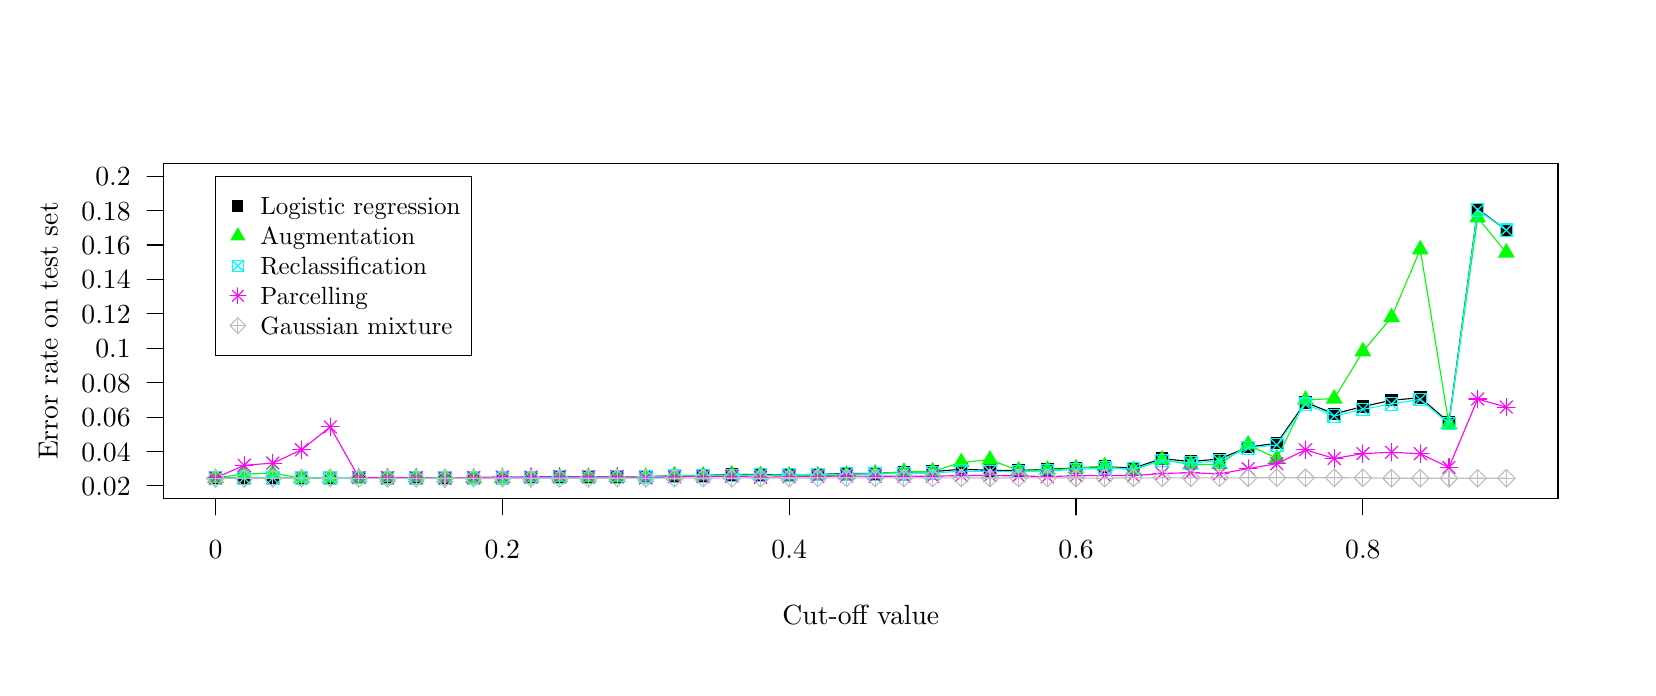
\begin{tikzpicture}[x=1pt,y=1pt]
\definecolor{fillColor}{RGB}{255,255,255}
\path[use as bounding box,fill=fillColor,fill opacity=0.00] (0,0) rectangle (578.16,231.26);
\begin{scope}
\path[clip] ( 49.20, 61.20) rectangle (552.96,182.06);
\definecolor{drawColor}{RGB}{0,0,0}

\path[draw=drawColor,line width= 0.4pt,line join=round,line cap=round] ( 67.86, 68.55) --
	( 78.22, 68.54) --
	( 88.59, 68.40) --
	( 98.95, 68.49) --
	(109.32, 68.56) --
	(119.68, 68.49) --
	(130.05, 68.56) --
	(140.42, 68.56) --
	(150.78, 68.56) --
	(161.15, 68.60) --
	(171.51, 68.69) --
	(181.88, 68.62) --
	(192.24, 68.69) --
	(202.61, 68.77) --
	(212.97, 68.90) --
	(223.34, 69.03) --
	(233.70, 69.35) --
	(244.07, 69.46) --
	(254.44, 69.79) --
	(264.80, 69.79) --
	(275.17, 69.69) --
	(285.53, 69.85) --
	(295.90, 70.17) --
	(306.26, 70.16) --
	(316.63, 70.68) --
	(326.99, 70.82) --
	(337.36, 71.71) --
	(347.72, 71.32) --
	(358.09, 71.28) --
	(368.46, 71.66) --
	(378.82, 72.19) --
	(389.19, 72.63) --
	(399.55, 72.11) --
	(409.92, 75.53) --
	(420.28, 74.46) --
	(430.65, 75.43) --
	(441.01, 79.67) --
	(451.38, 81.13) --
	(461.74, 95.88) --
	(472.11, 91.70) --
	(482.48, 94.35) --
	(492.84, 96.62) --
	(503.21, 97.55) --
	(513.57, 88.67) --
	(523.94,165.74) --
	(534.30,158.10);
\definecolor{fillColor}{RGB}{0,0,0}

\path[fill=fillColor] ( 65.61, 66.30) --
	( 70.11, 66.30) --
	( 70.11, 70.80) --
	( 65.61, 70.80) --
	cycle;

\path[fill=fillColor] ( 75.97, 66.29) --
	( 80.47, 66.29) --
	( 80.47, 70.79) --
	( 75.97, 70.79) --
	cycle;

\path[fill=fillColor] ( 86.34, 66.15) --
	( 90.84, 66.15) --
	( 90.84, 70.65) --
	( 86.34, 70.65) --
	cycle;

\path[fill=fillColor] ( 96.70, 66.24) --
	(101.20, 66.24) --
	(101.20, 70.74) --
	( 96.70, 70.74) --
	cycle;

\path[fill=fillColor] (107.07, 66.31) --
	(111.57, 66.31) --
	(111.57, 70.81) --
	(107.07, 70.81) --
	cycle;

\path[fill=fillColor] (117.43, 66.24) --
	(121.93, 66.24) --
	(121.93, 70.74) --
	(117.43, 70.74) --
	cycle;

\path[fill=fillColor] (127.80, 66.31) --
	(132.30, 66.31) --
	(132.30, 70.81) --
	(127.80, 70.81) --
	cycle;

\path[fill=fillColor] (138.17, 66.31) --
	(142.67, 66.31) --
	(142.67, 70.81) --
	(138.17, 70.81) --
	cycle;

\path[fill=fillColor] (148.53, 66.31) --
	(153.03, 66.31) --
	(153.03, 70.81) --
	(148.53, 70.81) --
	cycle;

\path[fill=fillColor] (158.90, 66.35) --
	(163.40, 66.35) --
	(163.40, 70.85) --
	(158.90, 70.85) --
	cycle;

\path[fill=fillColor] (169.26, 66.44) --
	(173.76, 66.44) --
	(173.76, 70.94) --
	(169.26, 70.94) --
	cycle;

\path[fill=fillColor] (179.63, 66.37) --
	(184.13, 66.37) --
	(184.13, 70.87) --
	(179.63, 70.87) --
	cycle;

\path[fill=fillColor] (189.99, 66.44) --
	(194.49, 66.44) --
	(194.49, 70.94) --
	(189.99, 70.94) --
	cycle;

\path[fill=fillColor] (200.36, 66.52) --
	(204.86, 66.52) --
	(204.86, 71.02) --
	(200.36, 71.02) --
	cycle;

\path[fill=fillColor] (210.72, 66.65) --
	(215.22, 66.65) --
	(215.22, 71.15) --
	(210.72, 71.15) --
	cycle;

\path[fill=fillColor] (221.09, 66.78) --
	(225.59, 66.78) --
	(225.59, 71.28) --
	(221.09, 71.28) --
	cycle;

\path[fill=fillColor] (231.45, 67.10) --
	(235.95, 67.10) --
	(235.95, 71.60) --
	(231.45, 71.60) --
	cycle;

\path[fill=fillColor] (241.82, 67.21) --
	(246.32, 67.21) --
	(246.32, 71.71) --
	(241.82, 71.71) --
	cycle;

\path[fill=fillColor] (252.19, 67.54) --
	(256.69, 67.54) --
	(256.69, 72.04) --
	(252.19, 72.04) --
	cycle;

\path[fill=fillColor] (262.55, 67.54) --
	(267.05, 67.54) --
	(267.05, 72.04) --
	(262.55, 72.04) --
	cycle;

\path[fill=fillColor] (272.92, 67.44) --
	(277.42, 67.44) --
	(277.42, 71.94) --
	(272.92, 71.94) --
	cycle;

\path[fill=fillColor] (283.28, 67.60) --
	(287.78, 67.60) --
	(287.78, 72.10) --
	(283.28, 72.10) --
	cycle;

\path[fill=fillColor] (293.65, 67.92) --
	(298.15, 67.92) --
	(298.15, 72.42) --
	(293.65, 72.42) --
	cycle;

\path[fill=fillColor] (304.01, 67.91) --
	(308.51, 67.91) --
	(308.51, 72.41) --
	(304.01, 72.41) --
	cycle;

\path[fill=fillColor] (314.38, 68.43) --
	(318.88, 68.43) --
	(318.88, 72.93) --
	(314.38, 72.93) --
	cycle;

\path[fill=fillColor] (324.74, 68.57) --
	(329.24, 68.57) --
	(329.24, 73.07) --
	(324.74, 73.07) --
	cycle;

\path[fill=fillColor] (335.11, 69.46) --
	(339.61, 69.46) --
	(339.61, 73.96) --
	(335.11, 73.96) --
	cycle;

\path[fill=fillColor] (345.47, 69.07) --
	(349.97, 69.07) --
	(349.97, 73.57) --
	(345.47, 73.57) --
	cycle;

\path[fill=fillColor] (355.84, 69.03) --
	(360.34, 69.03) --
	(360.34, 73.53) --
	(355.84, 73.53) --
	cycle;

\path[fill=fillColor] (366.21, 69.41) --
	(370.71, 69.41) --
	(370.71, 73.91) --
	(366.21, 73.91) --
	cycle;

\path[fill=fillColor] (376.57, 69.94) --
	(381.07, 69.94) --
	(381.07, 74.44) --
	(376.57, 74.44) --
	cycle;

\path[fill=fillColor] (386.94, 70.38) --
	(391.44, 70.38) --
	(391.44, 74.88) --
	(386.94, 74.88) --
	cycle;

\path[fill=fillColor] (397.30, 69.86) --
	(401.80, 69.86) --
	(401.80, 74.36) --
	(397.30, 74.36) --
	cycle;

\path[fill=fillColor] (407.67, 73.28) --
	(412.17, 73.28) --
	(412.17, 77.78) --
	(407.67, 77.78) --
	cycle;

\path[fill=fillColor] (418.03, 72.21) --
	(422.53, 72.21) --
	(422.53, 76.71) --
	(418.03, 76.71) --
	cycle;

\path[fill=fillColor] (428.40, 73.18) --
	(432.90, 73.18) --
	(432.90, 77.68) --
	(428.40, 77.68) --
	cycle;

\path[fill=fillColor] (438.76, 77.42) --
	(443.26, 77.42) --
	(443.26, 81.92) --
	(438.76, 81.92) --
	cycle;

\path[fill=fillColor] (449.13, 78.88) --
	(453.63, 78.88) --
	(453.63, 83.38) --
	(449.13, 83.38) --
	cycle;

\path[fill=fillColor] (459.49, 93.63) --
	(463.99, 93.63) --
	(463.99, 98.13) --
	(459.49, 98.13) --
	cycle;

\path[fill=fillColor] (469.86, 89.45) --
	(474.36, 89.45) --
	(474.36, 93.95) --
	(469.86, 93.95) --
	cycle;

\path[fill=fillColor] (480.23, 92.10) --
	(484.73, 92.10) --
	(484.73, 96.60) --
	(480.23, 96.60) --
	cycle;

\path[fill=fillColor] (490.59, 94.37) --
	(495.09, 94.37) --
	(495.09, 98.87) --
	(490.59, 98.87) --
	cycle;

\path[fill=fillColor] (500.96, 95.30) --
	(505.46, 95.30) --
	(505.46, 99.80) --
	(500.96, 99.80) --
	cycle;

\path[fill=fillColor] (511.32, 86.42) --
	(515.82, 86.42) --
	(515.82, 90.92) --
	(511.32, 90.92) --
	cycle;

\path[fill=fillColor] (521.69,163.49) --
	(526.19,163.49) --
	(526.19,167.99) --
	(521.69,167.99) --
	cycle;

\path[fill=fillColor] (532.05,155.85) --
	(536.55,155.85) --
	(536.55,160.35) --
	(532.05,160.35) --
	cycle;
\end{scope}
\begin{scope}
\path[clip] (  0.00,  0.00) rectangle (578.16,231.26);
\definecolor{drawColor}{RGB}{0,0,0}

\path[draw=drawColor,line width= 0.4pt,line join=round,line cap=round] ( 49.20, 61.20) --
	(552.96, 61.20) --
	(552.96,182.06) --
	( 49.20,182.06) --
	( 49.20, 61.20);
\end{scope}
\begin{scope}
\path[clip] (  0.00,  0.00) rectangle (578.16,231.26);
\definecolor{drawColor}{RGB}{0,0,0}

\node[text=drawColor,anchor=base,inner sep=0pt, outer sep=0pt, scale=  1.00] at (301.08, 15.60) {Cut-off value};

\node[text=drawColor,rotate= 90.00,anchor=base,inner sep=0pt, outer sep=0pt, scale=  1.00] at ( 10.80,121.63) {Error rate on test set};
\end{scope}
\begin{scope}
\path[clip] ( 49.20, 61.20) rectangle (552.96,182.06);
\definecolor{drawColor}{RGB}{0,255,0}

\path[draw=drawColor,line width= 0.4pt,line join=round,line cap=round] ( 67.86, 68.55) --
	( 78.22, 69.97) --
	( 88.59, 70.22) --
	( 98.95, 68.50) --
	(109.32, 68.59) --
	(119.68, 68.62) --
	(130.05, 68.75) --
	(140.42, 68.80) --
	(150.78, 68.59) --
	(161.15, 68.53) --
	(171.51, 68.49) --
	(181.88, 68.72) --
	(192.24, 68.83) --
	(202.61, 68.79) --
	(212.97, 68.82) --
	(223.34, 68.95) --
	(233.70, 69.43) --
	(244.07, 69.41) --
	(254.44, 69.77) --
	(264.80, 69.54) --
	(275.17, 69.33) --
	(285.53, 69.39) --
	(295.90, 69.65) --
	(306.26, 70.13) --
	(316.63, 70.74) --
	(326.99, 70.85) --
	(337.36, 74.20) --
	(347.72, 75.15) --
	(358.09, 71.21) --
	(368.46, 71.50) --
	(378.82, 72.01) --
	(389.19, 72.80) --
	(399.55, 71.35) --
	(409.92, 75.16) --
	(420.28, 73.40) --
	(430.65, 73.47) --
	(441.01, 80.59) --
	(451.38, 75.56) --
	(461.74, 96.78) --
	(472.11, 97.20) --
	(482.48,114.26) --
	(492.84,126.62) --
	(503.21,151.11) --
	(513.57, 88.00) --
	(523.94,162.63) --
	(534.30,149.95);
\definecolor{fillColor}{RGB}{0,255,0}

\path[fill=fillColor] ( 67.86, 72.05) --
	( 70.89, 66.80) --
	( 64.83, 66.80) --
	cycle;

\path[fill=fillColor] ( 78.22, 73.47) --
	( 81.25, 68.22) --
	( 75.19, 68.22) --
	cycle;

\path[fill=fillColor] ( 88.59, 73.72) --
	( 91.62, 68.47) --
	( 85.56, 68.47) --
	cycle;

\path[fill=fillColor] ( 98.95, 72.00) --
	(101.98, 66.75) --
	( 95.92, 66.75) --
	cycle;

\path[fill=fillColor] (109.32, 72.09) --
	(112.35, 66.84) --
	(106.29, 66.84) --
	cycle;

\path[fill=fillColor] (119.68, 72.12) --
	(122.72, 66.87) --
	(116.65, 66.87) --
	cycle;

\path[fill=fillColor] (130.05, 72.25) --
	(133.08, 67.00) --
	(127.02, 67.00) --
	cycle;

\path[fill=fillColor] (140.42, 72.30) --
	(143.45, 67.05) --
	(137.39, 67.05) --
	cycle;

\path[fill=fillColor] (150.78, 72.09) --
	(153.81, 66.84) --
	(147.75, 66.84) --
	cycle;

\path[fill=fillColor] (161.15, 72.03) --
	(164.18, 66.78) --
	(158.12, 66.78) --
	cycle;

\path[fill=fillColor] (171.51, 71.99) --
	(174.54, 66.74) --
	(168.48, 66.74) --
	cycle;

\path[fill=fillColor] (181.88, 72.22) --
	(184.91, 66.97) --
	(178.85, 66.97) --
	cycle;

\path[fill=fillColor] (192.24, 72.33) --
	(195.27, 67.08) --
	(189.21, 67.08) --
	cycle;

\path[fill=fillColor] (202.61, 72.28) --
	(205.64, 67.04) --
	(199.58, 67.04) --
	cycle;

\path[fill=fillColor] (212.97, 72.32) --
	(216.00, 67.07) --
	(209.94, 67.07) --
	cycle;

\path[fill=fillColor] (223.34, 72.45) --
	(226.37, 67.20) --
	(220.31, 67.20) --
	cycle;

\path[fill=fillColor] (233.70, 72.92) --
	(236.73, 67.68) --
	(230.67, 67.68) --
	cycle;

\path[fill=fillColor] (244.07, 72.91) --
	(247.10, 67.66) --
	(241.04, 67.66) --
	cycle;

\path[fill=fillColor] (254.44, 73.27) --
	(257.47, 68.02) --
	(251.41, 68.02) --
	cycle;

\path[fill=fillColor] (264.80, 73.04) --
	(267.83, 67.79) --
	(261.77, 67.79) --
	cycle;

\path[fill=fillColor] (275.17, 72.83) --
	(278.20, 67.58) --
	(272.14, 67.58) --
	cycle;

\path[fill=fillColor] (285.53, 72.89) --
	(288.56, 67.64) --
	(282.50, 67.64) --
	cycle;

\path[fill=fillColor] (295.90, 73.15) --
	(298.93, 67.90) --
	(292.87, 67.90) --
	cycle;

\path[fill=fillColor] (306.26, 73.63) --
	(309.29, 68.38) --
	(303.23, 68.38) --
	cycle;

\path[fill=fillColor] (316.63, 74.24) --
	(319.66, 68.99) --
	(313.60, 68.99) --
	cycle;

\path[fill=fillColor] (326.99, 74.35) --
	(330.02, 69.10) --
	(323.96, 69.10) --
	cycle;

\path[fill=fillColor] (337.36, 77.70) --
	(340.39, 72.45) --
	(334.33, 72.45) --
	cycle;

\path[fill=fillColor] (347.72, 78.64) --
	(350.75, 73.40) --
	(344.69, 73.40) --
	cycle;

\path[fill=fillColor] (358.09, 74.71) --
	(361.12, 69.46) --
	(355.06, 69.46) --
	cycle;

\path[fill=fillColor] (368.46, 75.00) --
	(371.49, 69.75) --
	(365.43, 69.75) --
	cycle;

\path[fill=fillColor] (378.82, 75.50) --
	(381.85, 70.26) --
	(375.79, 70.26) --
	cycle;

\path[fill=fillColor] (389.19, 76.29) --
	(392.22, 71.05) --
	(386.16, 71.05) --
	cycle;

\path[fill=fillColor] (399.55, 74.85) --
	(402.58, 69.60) --
	(396.52, 69.60) --
	cycle;

\path[fill=fillColor] (409.92, 78.66) --
	(412.95, 73.41) --
	(406.89, 73.41) --
	cycle;

\path[fill=fillColor] (420.28, 76.90) --
	(423.31, 71.66) --
	(417.25, 71.66) --
	cycle;

\path[fill=fillColor] (430.65, 76.97) --
	(433.68, 71.72) --
	(427.62, 71.72) --
	cycle;

\path[fill=fillColor] (441.01, 84.09) --
	(444.04, 78.84) --
	(437.98, 78.84) --
	cycle;

\path[fill=fillColor] (451.38, 79.05) --
	(454.41, 73.81) --
	(448.35, 73.81) --
	cycle;

\path[fill=fillColor] (461.74,100.27) --
	(464.77, 95.03) --
	(458.71, 95.03) --
	cycle;

\path[fill=fillColor] (472.11,100.70) --
	(475.14, 95.45) --
	(469.08, 95.45) --
	cycle;

\path[fill=fillColor] (482.48,117.76) --
	(485.51,112.52) --
	(479.44,112.52) --
	cycle;

\path[fill=fillColor] (492.84,130.12) --
	(495.87,124.87) --
	(489.81,124.87) --
	cycle;

\path[fill=fillColor] (503.21,154.61) --
	(506.24,149.36) --
	(500.18,149.36) --
	cycle;

\path[fill=fillColor] (513.57, 91.50) --
	(516.60, 86.25) --
	(510.54, 86.25) --
	cycle;

\path[fill=fillColor] (523.94,166.13) --
	(526.97,160.88) --
	(520.91,160.88) --
	cycle;

\path[fill=fillColor] (534.30,153.45) --
	(537.33,148.20) --
	(531.27,148.20) --
	cycle;
\end{scope}
\begin{scope}
\path[clip] (  0.00,  0.00) rectangle (578.16,231.26);
\definecolor{drawColor}{RGB}{0,0,0}

\path[draw=drawColor,line width= 0.4pt,line join=round,line cap=round] ( 49.20, 61.20) --
	(552.96, 61.20) --
	(552.96,182.06) --
	( 49.20,182.06) --
	( 49.20, 61.20);
\end{scope}
\begin{scope}
\path[clip] (  0.00,  0.00) rectangle (578.16,231.26);
\definecolor{drawColor}{RGB}{0,0,0}

%\node[text=drawColor,anchor=base,inner sep=0pt, outer sep=0pt, scale=  1.00] at (301.08, 15.60) {Cut-off value};

%\node[text=drawColor,rotate= 90.00,anchor=base,inner sep=0pt, outer sep=0pt, scale=  1.00] at ( 10.80,121.63) {Error rate on test set};
\end{scope}
\begin{scope}
\path[clip] ( 49.20, 61.20) rectangle (552.96,182.06);
\definecolor{drawColor}{RGB}{0,255,255}

\path[draw=drawColor,line width= 0.4pt,line join=round,line cap=round] ( 67.86, 68.55) --
	( 78.22, 68.51) --
	( 88.59, 68.52) --
	( 98.95, 68.56) --
	(109.32, 68.59) --
	(119.68, 68.64) --
	(130.05, 68.61) --
	(140.42, 68.60) --
	(150.78, 68.59) --
	(161.15, 68.61) --
	(171.51, 68.61) --
	(181.88, 68.69) --
	(192.24, 68.85) --
	(202.61, 68.85) --
	(212.97, 68.92) --
	(223.34, 68.98) --
	(233.70, 69.16) --
	(244.07, 69.31) --
	(254.44, 69.43) --
	(264.80, 69.57) --
	(275.17, 69.64) --
	(285.53, 69.82) --
	(295.90, 70.01) --
	(306.26, 69.98) --
	(316.63, 70.06) --
	(326.99, 70.30) --
	(337.36, 71.00) --
	(347.72, 70.89) --
	(358.09, 70.81) --
	(368.46, 71.05) --
	(378.82, 71.61) --
	(389.19, 72.17) --
	(399.55, 71.79) --
	(409.92, 74.87) --
	(420.28, 73.96) --
	(430.65, 74.69) --
	(441.01, 79.39) --
	(451.38, 80.44) --
	(461.74, 95.21) --
	(472.11, 90.92) --
	(482.48, 93.36) --
	(492.84, 95.30) --
	(503.21, 96.93) --
	(513.57, 88.18) --
	(523.94,165.41) --
	(534.30,158.07);

\path[draw=drawColor,line width= 0.4pt,line join=round,line cap=round] ( 65.61, 66.30) rectangle ( 70.11, 70.80);

\path[draw=drawColor,line width= 0.4pt,line join=round,line cap=round] ( 65.61, 66.30) -- ( 70.11, 70.80);

\path[draw=drawColor,line width= 0.4pt,line join=round,line cap=round] ( 65.61, 70.80) -- ( 70.11, 66.30);

\path[draw=drawColor,line width= 0.4pt,line join=round,line cap=round] ( 75.97, 66.26) rectangle ( 80.47, 70.76);

\path[draw=drawColor,line width= 0.4pt,line join=round,line cap=round] ( 75.97, 66.26) -- ( 80.47, 70.76);

\path[draw=drawColor,line width= 0.4pt,line join=round,line cap=round] ( 75.97, 70.76) -- ( 80.47, 66.26);

\path[draw=drawColor,line width= 0.4pt,line join=round,line cap=round] ( 86.34, 66.27) rectangle ( 90.84, 70.77);

\path[draw=drawColor,line width= 0.4pt,line join=round,line cap=round] ( 86.34, 66.27) -- ( 90.84, 70.77);

\path[draw=drawColor,line width= 0.4pt,line join=round,line cap=round] ( 86.34, 70.77) -- ( 90.84, 66.27);

\path[draw=drawColor,line width= 0.4pt,line join=round,line cap=round] ( 96.70, 66.31) rectangle (101.20, 70.81);

\path[draw=drawColor,line width= 0.4pt,line join=round,line cap=round] ( 96.70, 66.31) -- (101.20, 70.81);

\path[draw=drawColor,line width= 0.4pt,line join=round,line cap=round] ( 96.70, 70.81) -- (101.20, 66.31);

\path[draw=drawColor,line width= 0.4pt,line join=round,line cap=round] (107.07, 66.34) rectangle (111.57, 70.84);

\path[draw=drawColor,line width= 0.4pt,line join=round,line cap=round] (107.07, 66.34) -- (111.57, 70.84);

\path[draw=drawColor,line width= 0.4pt,line join=round,line cap=round] (107.07, 70.84) -- (111.57, 66.34);

\path[draw=drawColor,line width= 0.4pt,line join=round,line cap=round] (117.43, 66.39) rectangle (121.93, 70.89);

\path[draw=drawColor,line width= 0.4pt,line join=round,line cap=round] (117.43, 66.39) -- (121.93, 70.89);

\path[draw=drawColor,line width= 0.4pt,line join=round,line cap=round] (117.43, 70.89) -- (121.93, 66.39);

\path[draw=drawColor,line width= 0.4pt,line join=round,line cap=round] (127.80, 66.36) rectangle (132.30, 70.86);

\path[draw=drawColor,line width= 0.4pt,line join=round,line cap=round] (127.80, 66.36) -- (132.30, 70.86);

\path[draw=drawColor,line width= 0.4pt,line join=round,line cap=round] (127.80, 70.86) -- (132.30, 66.36);

\path[draw=drawColor,line width= 0.4pt,line join=round,line cap=round] (138.17, 66.35) rectangle (142.67, 70.85);

\path[draw=drawColor,line width= 0.4pt,line join=round,line cap=round] (138.17, 66.35) -- (142.67, 70.85);

\path[draw=drawColor,line width= 0.4pt,line join=round,line cap=round] (138.17, 70.85) -- (142.67, 66.35);

\path[draw=drawColor,line width= 0.4pt,line join=round,line cap=round] (148.53, 66.34) rectangle (153.03, 70.84);

\path[draw=drawColor,line width= 0.4pt,line join=round,line cap=round] (148.53, 66.34) -- (153.03, 70.84);

\path[draw=drawColor,line width= 0.4pt,line join=round,line cap=round] (148.53, 70.84) -- (153.03, 66.34);

\path[draw=drawColor,line width= 0.4pt,line join=round,line cap=round] (158.90, 66.36) rectangle (163.40, 70.86);

\path[draw=drawColor,line width= 0.4pt,line join=round,line cap=round] (158.90, 66.36) -- (163.40, 70.86);

\path[draw=drawColor,line width= 0.4pt,line join=round,line cap=round] (158.90, 70.86) -- (163.40, 66.36);

\path[draw=drawColor,line width= 0.4pt,line join=round,line cap=round] (169.26, 66.36) rectangle (173.76, 70.86);

\path[draw=drawColor,line width= 0.4pt,line join=round,line cap=round] (169.26, 66.36) -- (173.76, 70.86);

\path[draw=drawColor,line width= 0.4pt,line join=round,line cap=round] (169.26, 70.86) -- (173.76, 66.36);

\path[draw=drawColor,line width= 0.4pt,line join=round,line cap=round] (179.63, 66.44) rectangle (184.13, 70.94);

\path[draw=drawColor,line width= 0.4pt,line join=round,line cap=round] (179.63, 66.44) -- (184.13, 70.94);

\path[draw=drawColor,line width= 0.4pt,line join=round,line cap=round] (179.63, 70.94) -- (184.13, 66.44);

\path[draw=drawColor,line width= 0.4pt,line join=round,line cap=round] (189.99, 66.60) rectangle (194.49, 71.10);

\path[draw=drawColor,line width= 0.4pt,line join=round,line cap=round] (189.99, 66.60) -- (194.49, 71.10);

\path[draw=drawColor,line width= 0.4pt,line join=round,line cap=round] (189.99, 71.10) -- (194.49, 66.60);

\path[draw=drawColor,line width= 0.4pt,line join=round,line cap=round] (200.36, 66.60) rectangle (204.86, 71.10);

\path[draw=drawColor,line width= 0.4pt,line join=round,line cap=round] (200.36, 66.60) -- (204.86, 71.10);

\path[draw=drawColor,line width= 0.4pt,line join=round,line cap=round] (200.36, 71.10) -- (204.86, 66.60);

\path[draw=drawColor,line width= 0.4pt,line join=round,line cap=round] (210.72, 66.67) rectangle (215.22, 71.17);

\path[draw=drawColor,line width= 0.4pt,line join=round,line cap=round] (210.72, 66.67) -- (215.22, 71.17);

\path[draw=drawColor,line width= 0.4pt,line join=round,line cap=round] (210.72, 71.17) -- (215.22, 66.67);

\path[draw=drawColor,line width= 0.4pt,line join=round,line cap=round] (221.09, 66.73) rectangle (225.59, 71.23);

\path[draw=drawColor,line width= 0.4pt,line join=round,line cap=round] (221.09, 66.73) -- (225.59, 71.23);

\path[draw=drawColor,line width= 0.4pt,line join=round,line cap=round] (221.09, 71.23) -- (225.59, 66.73);

\path[draw=drawColor,line width= 0.4pt,line join=round,line cap=round] (231.45, 66.91) rectangle (235.95, 71.41);

\path[draw=drawColor,line width= 0.4pt,line join=round,line cap=round] (231.45, 66.91) -- (235.95, 71.41);

\path[draw=drawColor,line width= 0.4pt,line join=round,line cap=round] (231.45, 71.41) -- (235.95, 66.91);

\path[draw=drawColor,line width= 0.4pt,line join=round,line cap=round] (241.82, 67.06) rectangle (246.32, 71.56);

\path[draw=drawColor,line width= 0.4pt,line join=round,line cap=round] (241.82, 67.06) -- (246.32, 71.56);

\path[draw=drawColor,line width= 0.4pt,line join=round,line cap=round] (241.82, 71.56) -- (246.32, 67.06);

\path[draw=drawColor,line width= 0.4pt,line join=round,line cap=round] (252.19, 67.18) rectangle (256.69, 71.68);

\path[draw=drawColor,line width= 0.4pt,line join=round,line cap=round] (252.19, 67.18) -- (256.69, 71.68);

\path[draw=drawColor,line width= 0.4pt,line join=round,line cap=round] (252.19, 71.68) -- (256.69, 67.18);

\path[draw=drawColor,line width= 0.4pt,line join=round,line cap=round] (262.55, 67.32) rectangle (267.05, 71.82);

\path[draw=drawColor,line width= 0.4pt,line join=round,line cap=round] (262.55, 67.32) -- (267.05, 71.82);

\path[draw=drawColor,line width= 0.4pt,line join=round,line cap=round] (262.55, 71.82) -- (267.05, 67.32);

\path[draw=drawColor,line width= 0.4pt,line join=round,line cap=round] (272.92, 67.39) rectangle (277.42, 71.89);

\path[draw=drawColor,line width= 0.4pt,line join=round,line cap=round] (272.92, 67.39) -- (277.42, 71.89);

\path[draw=drawColor,line width= 0.4pt,line join=round,line cap=round] (272.92, 71.89) -- (277.42, 67.39);

\path[draw=drawColor,line width= 0.4pt,line join=round,line cap=round] (283.28, 67.57) rectangle (287.78, 72.07);

\path[draw=drawColor,line width= 0.4pt,line join=round,line cap=round] (283.28, 67.57) -- (287.78, 72.07);

\path[draw=drawColor,line width= 0.4pt,line join=round,line cap=round] (283.28, 72.07) -- (287.78, 67.57);

\path[draw=drawColor,line width= 0.4pt,line join=round,line cap=round] (293.65, 67.76) rectangle (298.15, 72.26);

\path[draw=drawColor,line width= 0.4pt,line join=round,line cap=round] (293.65, 67.76) -- (298.15, 72.26);

\path[draw=drawColor,line width= 0.4pt,line join=round,line cap=round] (293.65, 72.26) -- (298.15, 67.76);

\path[draw=drawColor,line width= 0.4pt,line join=round,line cap=round] (304.01, 67.73) rectangle (308.51, 72.23);

\path[draw=drawColor,line width= 0.4pt,line join=round,line cap=round] (304.01, 67.73) -- (308.51, 72.23);

\path[draw=drawColor,line width= 0.4pt,line join=round,line cap=round] (304.01, 72.23) -- (308.51, 67.73);

\path[draw=drawColor,line width= 0.4pt,line join=round,line cap=round] (314.38, 67.81) rectangle (318.88, 72.31);

\path[draw=drawColor,line width= 0.4pt,line join=round,line cap=round] (314.38, 67.81) -- (318.88, 72.31);

\path[draw=drawColor,line width= 0.4pt,line join=round,line cap=round] (314.38, 72.31) -- (318.88, 67.81);

\path[draw=drawColor,line width= 0.4pt,line join=round,line cap=round] (324.74, 68.05) rectangle (329.24, 72.55);

\path[draw=drawColor,line width= 0.4pt,line join=round,line cap=round] (324.74, 68.05) -- (329.24, 72.55);

\path[draw=drawColor,line width= 0.4pt,line join=round,line cap=round] (324.74, 72.55) -- (329.24, 68.05);

\path[draw=drawColor,line width= 0.4pt,line join=round,line cap=round] (335.11, 68.75) rectangle (339.61, 73.25);

\path[draw=drawColor,line width= 0.4pt,line join=round,line cap=round] (335.11, 68.75) -- (339.61, 73.25);

\path[draw=drawColor,line width= 0.4pt,line join=round,line cap=round] (335.11, 73.25) -- (339.61, 68.75);

\path[draw=drawColor,line width= 0.4pt,line join=round,line cap=round] (345.47, 68.64) rectangle (349.97, 73.14);

\path[draw=drawColor,line width= 0.4pt,line join=round,line cap=round] (345.47, 68.64) -- (349.97, 73.14);

\path[draw=drawColor,line width= 0.4pt,line join=round,line cap=round] (345.47, 73.14) -- (349.97, 68.64);

\path[draw=drawColor,line width= 0.4pt,line join=round,line cap=round] (355.84, 68.56) rectangle (360.34, 73.06);

\path[draw=drawColor,line width= 0.4pt,line join=round,line cap=round] (355.84, 68.56) -- (360.34, 73.06);

\path[draw=drawColor,line width= 0.4pt,line join=round,line cap=round] (355.84, 73.06) -- (360.34, 68.56);

\path[draw=drawColor,line width= 0.4pt,line join=round,line cap=round] (366.21, 68.80) rectangle (370.71, 73.30);

\path[draw=drawColor,line width= 0.4pt,line join=round,line cap=round] (366.21, 68.80) -- (370.71, 73.30);

\path[draw=drawColor,line width= 0.4pt,line join=round,line cap=round] (366.21, 73.30) -- (370.71, 68.80);

\path[draw=drawColor,line width= 0.4pt,line join=round,line cap=round] (376.57, 69.36) rectangle (381.07, 73.86);

\path[draw=drawColor,line width= 0.4pt,line join=round,line cap=round] (376.57, 69.36) -- (381.07, 73.86);

\path[draw=drawColor,line width= 0.4pt,line join=round,line cap=round] (376.57, 73.86) -- (381.07, 69.36);

\path[draw=drawColor,line width= 0.4pt,line join=round,line cap=round] (386.94, 69.92) rectangle (391.44, 74.42);

\path[draw=drawColor,line width= 0.4pt,line join=round,line cap=round] (386.94, 69.92) -- (391.44, 74.42);

\path[draw=drawColor,line width= 0.4pt,line join=round,line cap=round] (386.94, 74.42) -- (391.44, 69.92);

\path[draw=drawColor,line width= 0.4pt,line join=round,line cap=round] (397.30, 69.54) rectangle (401.80, 74.04);

\path[draw=drawColor,line width= 0.4pt,line join=round,line cap=round] (397.30, 69.54) -- (401.80, 74.04);

\path[draw=drawColor,line width= 0.4pt,line join=round,line cap=round] (397.30, 74.04) -- (401.80, 69.54);

\path[draw=drawColor,line width= 0.4pt,line join=round,line cap=round] (407.67, 72.62) rectangle (412.17, 77.12);

\path[draw=drawColor,line width= 0.4pt,line join=round,line cap=round] (407.67, 72.62) -- (412.17, 77.12);

\path[draw=drawColor,line width= 0.4pt,line join=round,line cap=round] (407.67, 77.12) -- (412.17, 72.62);

\path[draw=drawColor,line width= 0.4pt,line join=round,line cap=round] (418.03, 71.71) rectangle (422.53, 76.21);

\path[draw=drawColor,line width= 0.4pt,line join=round,line cap=round] (418.03, 71.71) -- (422.53, 76.21);

\path[draw=drawColor,line width= 0.4pt,line join=round,line cap=round] (418.03, 76.21) -- (422.53, 71.71);

\path[draw=drawColor,line width= 0.4pt,line join=round,line cap=round] (428.40, 72.44) rectangle (432.90, 76.94);

\path[draw=drawColor,line width= 0.4pt,line join=round,line cap=round] (428.40, 72.44) -- (432.90, 76.94);

\path[draw=drawColor,line width= 0.4pt,line join=round,line cap=round] (428.40, 76.94) -- (432.90, 72.44);

\path[draw=drawColor,line width= 0.4pt,line join=round,line cap=round] (438.76, 77.14) rectangle (443.26, 81.64);

\path[draw=drawColor,line width= 0.4pt,line join=round,line cap=round] (438.76, 77.14) -- (443.26, 81.64);

\path[draw=drawColor,line width= 0.4pt,line join=round,line cap=round] (438.76, 81.64) -- (443.26, 77.14);

\path[draw=drawColor,line width= 0.4pt,line join=round,line cap=round] (449.13, 78.19) rectangle (453.63, 82.69);

\path[draw=drawColor,line width= 0.4pt,line join=round,line cap=round] (449.13, 78.19) -- (453.63, 82.69);

\path[draw=drawColor,line width= 0.4pt,line join=round,line cap=round] (449.13, 82.69) -- (453.63, 78.19);

\path[draw=drawColor,line width= 0.4pt,line join=round,line cap=round] (459.49, 92.96) rectangle (463.99, 97.46);

\path[draw=drawColor,line width= 0.4pt,line join=round,line cap=round] (459.49, 92.96) -- (463.99, 97.46);

\path[draw=drawColor,line width= 0.4pt,line join=round,line cap=round] (459.49, 97.46) -- (463.99, 92.96);

\path[draw=drawColor,line width= 0.4pt,line join=round,line cap=round] (469.86, 88.67) rectangle (474.36, 93.17);

\path[draw=drawColor,line width= 0.4pt,line join=round,line cap=round] (469.86, 88.67) -- (474.36, 93.17);

\path[draw=drawColor,line width= 0.4pt,line join=round,line cap=round] (469.86, 93.17) -- (474.36, 88.67);

\path[draw=drawColor,line width= 0.4pt,line join=round,line cap=round] (480.23, 91.11) rectangle (484.73, 95.61);

\path[draw=drawColor,line width= 0.4pt,line join=round,line cap=round] (480.23, 91.11) -- (484.73, 95.61);

\path[draw=drawColor,line width= 0.4pt,line join=round,line cap=round] (480.23, 95.61) -- (484.73, 91.11);

\path[draw=drawColor,line width= 0.4pt,line join=round,line cap=round] (490.59, 93.05) rectangle (495.09, 97.55);

\path[draw=drawColor,line width= 0.4pt,line join=round,line cap=round] (490.59, 93.05) -- (495.09, 97.55);

\path[draw=drawColor,line width= 0.4pt,line join=round,line cap=round] (490.59, 97.55) -- (495.09, 93.05);

\path[draw=drawColor,line width= 0.4pt,line join=round,line cap=round] (500.96, 94.68) rectangle (505.46, 99.18);

\path[draw=drawColor,line width= 0.4pt,line join=round,line cap=round] (500.96, 94.68) -- (505.46, 99.18);

\path[draw=drawColor,line width= 0.4pt,line join=round,line cap=round] (500.96, 99.18) -- (505.46, 94.68);

\path[draw=drawColor,line width= 0.4pt,line join=round,line cap=round] (511.32, 85.93) rectangle (515.82, 90.43);

\path[draw=drawColor,line width= 0.4pt,line join=round,line cap=round] (511.32, 85.93) -- (515.82, 90.43);

\path[draw=drawColor,line width= 0.4pt,line join=round,line cap=round] (511.32, 90.43) -- (515.82, 85.93);

\path[draw=drawColor,line width= 0.4pt,line join=round,line cap=round] (521.69,163.16) rectangle (526.19,167.66);

\path[draw=drawColor,line width= 0.4pt,line join=round,line cap=round] (521.69,163.16) -- (526.19,167.66);

\path[draw=drawColor,line width= 0.4pt,line join=round,line cap=round] (521.69,167.66) -- (526.19,163.16);

\path[draw=drawColor,line width= 0.4pt,line join=round,line cap=round] (532.05,155.82) rectangle (536.55,160.32);

\path[draw=drawColor,line width= 0.4pt,line join=round,line cap=round] (532.05,155.82) -- (536.55,160.32);

\path[draw=drawColor,line width= 0.4pt,line join=round,line cap=round] (532.05,160.32) -- (536.55,155.82);
\end{scope}
\begin{scope}
\path[clip] (  0.00,  0.00) rectangle (578.16,231.26);
\definecolor{drawColor}{RGB}{0,0,0}

\path[draw=drawColor,line width= 0.4pt,line join=round,line cap=round] ( 49.20, 61.20) --
	(552.96, 61.20) --
	(552.96,182.06) --
	( 49.20,182.06) --
	( 49.20, 61.20);
\end{scope}
\begin{scope}
\path[clip] (  0.00,  0.00) rectangle (578.16,231.26);
\definecolor{drawColor}{RGB}{0,0,0}

%\node[text=drawColor,anchor=base,inner sep=0pt, outer sep=0pt, scale=  1.00] at (301.08, 15.60) {Cut-off value};

%\node[text=drawColor,rotate= 90.00,anchor=base,inner sep=0pt, outer sep=0pt, scale=  1.00] at ( 10.80,121.63) {Error rate on test set};
\end{scope}
\begin{scope}
\path[clip] ( 49.20, 61.20) rectangle (552.96,182.06);
\definecolor{drawColor}{RGB}{255,0,255}

\path[draw=drawColor,line width= 0.4pt,line join=round,line cap=round] ( 67.86, 68.55) --
	( 78.22, 73.11) --
	( 88.59, 73.92) --
	( 98.95, 78.73) --
	(109.32, 87.00) --
	(119.68, 68.70) --
	(130.05, 68.69) --
	(140.42, 68.60) --
	(150.78, 68.42) --
	(161.15, 68.74) --
	(171.51, 68.92) --
	(181.88, 68.94) --
	(192.24, 69.12) --
	(202.61, 68.97) --
	(212.97, 69.10) --
	(223.34, 68.56) --
	(233.70, 69.00) --
	(244.07, 69.01) --
	(254.44, 69.18) --
	(264.80, 68.80) --
	(275.17, 68.97) --
	(285.53, 69.12) --
	(295.90, 69.26) --
	(306.26, 69.16) --
	(316.63, 69.20) --
	(326.99, 69.16) --
	(337.36, 69.44) --
	(347.72, 69.41) --
	(358.09, 69.31) --
	(368.46, 69.02) --
	(378.82, 69.34) --
	(389.19, 69.41) --
	(399.55, 69.36) --
	(409.92, 70.17) --
	(420.28, 70.43) --
	(430.65, 70.03) --
	(441.01, 71.91) --
	(451.38, 73.72) --
	(461.74, 78.70) --
	(472.11, 75.59) --
	(482.48, 77.35) --
	(492.84, 77.84) --
	(503.21, 77.30) --
	(513.57, 72.35) --
	(523.94, 97.07) --
	(534.30, 94.15);

\path[draw=drawColor,line width= 0.4pt,line join=round,line cap=round] ( 65.61, 66.30) -- ( 70.11, 70.80);

\path[draw=drawColor,line width= 0.4pt,line join=round,line cap=round] ( 65.61, 70.80) -- ( 70.11, 66.30);

\path[draw=drawColor,line width= 0.4pt,line join=round,line cap=round] ( 64.68, 68.55) -- ( 71.04, 68.55);

\path[draw=drawColor,line width= 0.4pt,line join=round,line cap=round] ( 67.86, 65.37) -- ( 67.86, 71.73);

\path[draw=drawColor,line width= 0.4pt,line join=round,line cap=round] ( 75.97, 70.86) -- ( 80.47, 75.36);

\path[draw=drawColor,line width= 0.4pt,line join=round,line cap=round] ( 75.97, 75.36) -- ( 80.47, 70.86);

\path[draw=drawColor,line width= 0.4pt,line join=round,line cap=round] ( 75.04, 73.11) -- ( 81.41, 73.11);

\path[draw=drawColor,line width= 0.4pt,line join=round,line cap=round] ( 78.22, 69.93) -- ( 78.22, 76.29);

\path[draw=drawColor,line width= 0.4pt,line join=round,line cap=round] ( 86.34, 71.67) -- ( 90.84, 76.17);

\path[draw=drawColor,line width= 0.4pt,line join=round,line cap=round] ( 86.34, 76.17) -- ( 90.84, 71.67);

\path[draw=drawColor,line width= 0.4pt,line join=round,line cap=round] ( 85.41, 73.92) -- ( 91.77, 73.92);

\path[draw=drawColor,line width= 0.4pt,line join=round,line cap=round] ( 88.59, 70.74) -- ( 88.59, 77.10);

\path[draw=drawColor,line width= 0.4pt,line join=round,line cap=round] ( 96.70, 76.48) -- (101.20, 80.98);

\path[draw=drawColor,line width= 0.4pt,line join=round,line cap=round] ( 96.70, 80.98) -- (101.20, 76.48);

\path[draw=drawColor,line width= 0.4pt,line join=round,line cap=round] ( 95.77, 78.73) -- (102.14, 78.73);

\path[draw=drawColor,line width= 0.4pt,line join=round,line cap=round] ( 98.95, 75.54) -- ( 98.95, 81.91);

\path[draw=drawColor,line width= 0.4pt,line join=round,line cap=round] (107.07, 84.75) -- (111.57, 89.25);

\path[draw=drawColor,line width= 0.4pt,line join=round,line cap=round] (107.07, 89.25) -- (111.57, 84.75);

\path[draw=drawColor,line width= 0.4pt,line join=round,line cap=round] (106.14, 87.00) -- (112.50, 87.00);

\path[draw=drawColor,line width= 0.4pt,line join=round,line cap=round] (109.32, 83.81) -- (109.32, 90.18);

\path[draw=drawColor,line width= 0.4pt,line join=round,line cap=round] (117.43, 66.45) -- (121.93, 70.95);

\path[draw=drawColor,line width= 0.4pt,line join=round,line cap=round] (117.43, 70.95) -- (121.93, 66.45);

\path[draw=drawColor,line width= 0.4pt,line join=round,line cap=round] (116.50, 68.70) -- (122.87, 68.70);

\path[draw=drawColor,line width= 0.4pt,line join=round,line cap=round] (119.68, 65.52) -- (119.68, 71.89);

\path[draw=drawColor,line width= 0.4pt,line join=round,line cap=round] (127.80, 66.44) -- (132.30, 70.94);

\path[draw=drawColor,line width= 0.4pt,line join=round,line cap=round] (127.80, 70.94) -- (132.30, 66.44);

\path[draw=drawColor,line width= 0.4pt,line join=round,line cap=round] (126.87, 68.69) -- (133.23, 68.69);

\path[draw=drawColor,line width= 0.4pt,line join=round,line cap=round] (130.05, 65.51) -- (130.05, 71.87);

\path[draw=drawColor,line width= 0.4pt,line join=round,line cap=round] (138.17, 66.35) -- (142.67, 70.85);

\path[draw=drawColor,line width= 0.4pt,line join=round,line cap=round] (138.17, 70.85) -- (142.67, 66.35);

\path[draw=drawColor,line width= 0.4pt,line join=round,line cap=round] (137.23, 68.60) -- (143.60, 68.60);

\path[draw=drawColor,line width= 0.4pt,line join=round,line cap=round] (140.42, 65.42) -- (140.42, 71.79);

\path[draw=drawColor,line width= 0.4pt,line join=round,line cap=round] (148.53, 66.17) -- (153.03, 70.67);

\path[draw=drawColor,line width= 0.4pt,line join=round,line cap=round] (148.53, 70.67) -- (153.03, 66.17);

\path[draw=drawColor,line width= 0.4pt,line join=round,line cap=round] (147.60, 68.42) -- (153.96, 68.42);

\path[draw=drawColor,line width= 0.4pt,line join=round,line cap=round] (150.78, 65.24) -- (150.78, 71.60);

\path[draw=drawColor,line width= 0.4pt,line join=round,line cap=round] (158.90, 66.49) -- (163.40, 70.99);

\path[draw=drawColor,line width= 0.4pt,line join=round,line cap=round] (158.90, 70.99) -- (163.40, 66.49);

\path[draw=drawColor,line width= 0.4pt,line join=round,line cap=round] (157.96, 68.74) -- (164.33, 68.74);

\path[draw=drawColor,line width= 0.4pt,line join=round,line cap=round] (161.15, 65.56) -- (161.15, 71.92);

\path[draw=drawColor,line width= 0.4pt,line join=round,line cap=round] (169.26, 66.67) -- (173.76, 71.17);

\path[draw=drawColor,line width= 0.4pt,line join=round,line cap=round] (169.26, 71.17) -- (173.76, 66.67);

\path[draw=drawColor,line width= 0.4pt,line join=round,line cap=round] (168.33, 68.92) -- (174.69, 68.92);

\path[draw=drawColor,line width= 0.4pt,line join=round,line cap=round] (171.51, 65.74) -- (171.51, 72.10);

\path[draw=drawColor,line width= 0.4pt,line join=round,line cap=round] (179.63, 66.69) -- (184.13, 71.19);

\path[draw=drawColor,line width= 0.4pt,line join=round,line cap=round] (179.63, 71.19) -- (184.13, 66.69);

\path[draw=drawColor,line width= 0.4pt,line join=round,line cap=round] (178.70, 68.94) -- (185.06, 68.94);

\path[draw=drawColor,line width= 0.4pt,line join=round,line cap=round] (181.88, 65.76) -- (181.88, 72.12);

\path[draw=drawColor,line width= 0.4pt,line join=round,line cap=round] (189.99, 66.87) -- (194.49, 71.37);

\path[draw=drawColor,line width= 0.4pt,line join=round,line cap=round] (189.99, 71.37) -- (194.49, 66.87);

\path[draw=drawColor,line width= 0.4pt,line join=round,line cap=round] (189.06, 69.12) -- (195.42, 69.12);

\path[draw=drawColor,line width= 0.4pt,line join=round,line cap=round] (192.24, 65.94) -- (192.24, 72.30);

\path[draw=drawColor,line width= 0.4pt,line join=round,line cap=round] (200.36, 66.72) -- (204.86, 71.22);

\path[draw=drawColor,line width= 0.4pt,line join=round,line cap=round] (200.36, 71.22) -- (204.86, 66.72);

\path[draw=drawColor,line width= 0.4pt,line join=round,line cap=round] (199.43, 68.97) -- (205.79, 68.97);

\path[draw=drawColor,line width= 0.4pt,line join=round,line cap=round] (202.61, 65.79) -- (202.61, 72.15);

\path[draw=drawColor,line width= 0.4pt,line join=round,line cap=round] (210.72, 66.85) -- (215.22, 71.35);

\path[draw=drawColor,line width= 0.4pt,line join=round,line cap=round] (210.72, 71.35) -- (215.22, 66.85);

\path[draw=drawColor,line width= 0.4pt,line join=round,line cap=round] (209.79, 69.10) -- (216.16, 69.10);

\path[draw=drawColor,line width= 0.4pt,line join=round,line cap=round] (212.97, 65.92) -- (212.97, 72.28);

\path[draw=drawColor,line width= 0.4pt,line join=round,line cap=round] (221.09, 66.31) -- (225.59, 70.81);

\path[draw=drawColor,line width= 0.4pt,line join=round,line cap=round] (221.09, 70.81) -- (225.59, 66.31);

\path[draw=drawColor,line width= 0.4pt,line join=round,line cap=round] (220.16, 68.56) -- (226.52, 68.56);

\path[draw=drawColor,line width= 0.4pt,line join=round,line cap=round] (223.34, 65.38) -- (223.34, 71.74);

\path[draw=drawColor,line width= 0.4pt,line join=round,line cap=round] (231.45, 66.75) -- (235.95, 71.25);

\path[draw=drawColor,line width= 0.4pt,line join=round,line cap=round] (231.45, 71.25) -- (235.95, 66.75);

\path[draw=drawColor,line width= 0.4pt,line join=round,line cap=round] (230.52, 69.00) -- (236.89, 69.00);

\path[draw=drawColor,line width= 0.4pt,line join=round,line cap=round] (233.70, 65.81) -- (233.70, 72.18);

\path[draw=drawColor,line width= 0.4pt,line join=round,line cap=round] (241.82, 66.76) -- (246.32, 71.26);

\path[draw=drawColor,line width= 0.4pt,line join=round,line cap=round] (241.82, 71.26) -- (246.32, 66.76);

\path[draw=drawColor,line width= 0.4pt,line join=round,line cap=round] (240.89, 69.01) -- (247.25, 69.01);

\path[draw=drawColor,line width= 0.4pt,line join=round,line cap=round] (244.07, 65.83) -- (244.07, 72.19);

\path[draw=drawColor,line width= 0.4pt,line join=round,line cap=round] (252.19, 66.93) -- (256.69, 71.43);

\path[draw=drawColor,line width= 0.4pt,line join=round,line cap=round] (252.19, 71.43) -- (256.69, 66.93);

\path[draw=drawColor,line width= 0.4pt,line join=round,line cap=round] (251.25, 69.18) -- (257.62, 69.18);

\path[draw=drawColor,line width= 0.4pt,line join=round,line cap=round] (254.44, 66.00) -- (254.44, 72.36);

\path[draw=drawColor,line width= 0.4pt,line join=round,line cap=round] (262.55, 66.55) -- (267.05, 71.05);

\path[draw=drawColor,line width= 0.4pt,line join=round,line cap=round] (262.55, 71.05) -- (267.05, 66.55);

\path[draw=drawColor,line width= 0.4pt,line join=round,line cap=round] (261.62, 68.80) -- (267.98, 68.80);

\path[draw=drawColor,line width= 0.4pt,line join=round,line cap=round] (264.80, 65.62) -- (264.80, 71.98);

\path[draw=drawColor,line width= 0.4pt,line join=round,line cap=round] (272.92, 66.72) -- (277.42, 71.22);

\path[draw=drawColor,line width= 0.4pt,line join=round,line cap=round] (272.92, 71.22) -- (277.42, 66.72);

\path[draw=drawColor,line width= 0.4pt,line join=round,line cap=round] (271.98, 68.97) -- (278.35, 68.97);

\path[draw=drawColor,line width= 0.4pt,line join=round,line cap=round] (275.17, 65.79) -- (275.17, 72.15);

\path[draw=drawColor,line width= 0.4pt,line join=round,line cap=round] (283.28, 66.87) -- (287.78, 71.37);

\path[draw=drawColor,line width= 0.4pt,line join=round,line cap=round] (283.28, 71.37) -- (287.78, 66.87);

\path[draw=drawColor,line width= 0.4pt,line join=round,line cap=round] (282.35, 69.12) -- (288.71, 69.12);

\path[draw=drawColor,line width= 0.4pt,line join=round,line cap=round] (285.53, 65.94) -- (285.53, 72.30);

\path[draw=drawColor,line width= 0.4pt,line join=round,line cap=round] (293.65, 67.01) -- (298.15, 71.51);

\path[draw=drawColor,line width= 0.4pt,line join=round,line cap=round] (293.65, 71.51) -- (298.15, 67.01);

\path[draw=drawColor,line width= 0.4pt,line join=round,line cap=round] (292.72, 69.26) -- (299.08, 69.26);

\path[draw=drawColor,line width= 0.4pt,line join=round,line cap=round] (295.90, 66.08) -- (295.90, 72.44);

\path[draw=drawColor,line width= 0.4pt,line join=round,line cap=round] (304.01, 66.91) -- (308.51, 71.41);

\path[draw=drawColor,line width= 0.4pt,line join=round,line cap=round] (304.01, 71.41) -- (308.51, 66.91);

\path[draw=drawColor,line width= 0.4pt,line join=round,line cap=round] (303.08, 69.16) -- (309.44, 69.16);

\path[draw=drawColor,line width= 0.4pt,line join=round,line cap=round] (306.26, 65.98) -- (306.26, 72.35);

\path[draw=drawColor,line width= 0.4pt,line join=round,line cap=round] (314.38, 66.95) -- (318.88, 71.45);

\path[draw=drawColor,line width= 0.4pt,line join=round,line cap=round] (314.38, 71.45) -- (318.88, 66.95);

\path[draw=drawColor,line width= 0.4pt,line join=round,line cap=round] (313.45, 69.20) -- (319.81, 69.20);

\path[draw=drawColor,line width= 0.4pt,line join=round,line cap=round] (316.63, 66.01) -- (316.63, 72.38);

\path[draw=drawColor,line width= 0.4pt,line join=round,line cap=round] (324.74, 66.91) -- (329.24, 71.41);

\path[draw=drawColor,line width= 0.4pt,line join=round,line cap=round] (324.74, 71.41) -- (329.24, 66.91);

\path[draw=drawColor,line width= 0.4pt,line join=round,line cap=round] (323.81, 69.16) -- (330.18, 69.16);

\path[draw=drawColor,line width= 0.4pt,line join=round,line cap=round] (326.99, 65.98) -- (326.99, 72.34);

\path[draw=drawColor,line width= 0.4pt,line join=round,line cap=round] (335.11, 67.19) -- (339.61, 71.69);

\path[draw=drawColor,line width= 0.4pt,line join=round,line cap=round] (335.11, 71.69) -- (339.61, 67.19);

\path[draw=drawColor,line width= 0.4pt,line join=round,line cap=round] (334.18, 69.44) -- (340.54, 69.44);

\path[draw=drawColor,line width= 0.4pt,line join=round,line cap=round] (337.36, 66.26) -- (337.36, 72.62);

\path[draw=drawColor,line width= 0.4pt,line join=round,line cap=round] (345.47, 67.16) -- (349.97, 71.66);

\path[draw=drawColor,line width= 0.4pt,line join=round,line cap=round] (345.47, 71.66) -- (349.97, 67.16);

\path[draw=drawColor,line width= 0.4pt,line join=round,line cap=round] (344.54, 69.41) -- (350.91, 69.41);

\path[draw=drawColor,line width= 0.4pt,line join=round,line cap=round] (347.72, 66.22) -- (347.72, 72.59);

\path[draw=drawColor,line width= 0.4pt,line join=round,line cap=round] (355.84, 67.06) -- (360.34, 71.56);

\path[draw=drawColor,line width= 0.4pt,line join=round,line cap=round] (355.84, 71.56) -- (360.34, 67.06);

\path[draw=drawColor,line width= 0.4pt,line join=round,line cap=round] (354.91, 69.31) -- (361.27, 69.31);

\path[draw=drawColor,line width= 0.4pt,line join=round,line cap=round] (358.09, 66.13) -- (358.09, 72.49);

\path[draw=drawColor,line width= 0.4pt,line join=round,line cap=round] (366.21, 66.77) -- (370.71, 71.27);

\path[draw=drawColor,line width= 0.4pt,line join=round,line cap=round] (366.21, 71.27) -- (370.71, 66.77);

\path[draw=drawColor,line width= 0.4pt,line join=round,line cap=round] (365.27, 69.02) -- (371.64, 69.02);

\path[draw=drawColor,line width= 0.4pt,line join=round,line cap=round] (368.46, 65.83) -- (368.46, 72.20);

\path[draw=drawColor,line width= 0.4pt,line join=round,line cap=round] (376.57, 67.09) -- (381.07, 71.59);

\path[draw=drawColor,line width= 0.4pt,line join=round,line cap=round] (376.57, 71.59) -- (381.07, 67.09);

\path[draw=drawColor,line width= 0.4pt,line join=round,line cap=round] (375.64, 69.34) -- (382.00, 69.34);

\path[draw=drawColor,line width= 0.4pt,line join=round,line cap=round] (378.82, 66.16) -- (378.82, 72.53);

\path[draw=drawColor,line width= 0.4pt,line join=round,line cap=round] (386.94, 67.16) -- (391.44, 71.66);

\path[draw=drawColor,line width= 0.4pt,line join=round,line cap=round] (386.94, 71.66) -- (391.44, 67.16);

\path[draw=drawColor,line width= 0.4pt,line join=round,line cap=round] (386.00, 69.41) -- (392.37, 69.41);

\path[draw=drawColor,line width= 0.4pt,line join=round,line cap=round] (389.19, 66.22) -- (389.19, 72.59);

\path[draw=drawColor,line width= 0.4pt,line join=round,line cap=round] (397.30, 67.11) -- (401.80, 71.61);

\path[draw=drawColor,line width= 0.4pt,line join=round,line cap=round] (397.30, 71.61) -- (401.80, 67.11);

\path[draw=drawColor,line width= 0.4pt,line join=round,line cap=round] (396.37, 69.36) -- (402.73, 69.36);

\path[draw=drawColor,line width= 0.4pt,line join=round,line cap=round] (399.55, 66.18) -- (399.55, 72.55);

\path[draw=drawColor,line width= 0.4pt,line join=round,line cap=round] (407.67, 67.92) -- (412.17, 72.42);

\path[draw=drawColor,line width= 0.4pt,line join=round,line cap=round] (407.67, 72.42) -- (412.17, 67.92);

\path[draw=drawColor,line width= 0.4pt,line join=round,line cap=round] (406.74, 70.17) -- (413.10, 70.17);

\path[draw=drawColor,line width= 0.4pt,line join=round,line cap=round] (409.92, 66.99) -- (409.92, 73.35);

\path[draw=drawColor,line width= 0.4pt,line join=round,line cap=round] (418.03, 68.18) -- (422.53, 72.68);

\path[draw=drawColor,line width= 0.4pt,line join=round,line cap=round] (418.03, 72.68) -- (422.53, 68.18);

\path[draw=drawColor,line width= 0.4pt,line join=round,line cap=round] (417.10, 70.43) -- (423.46, 70.43);

\path[draw=drawColor,line width= 0.4pt,line join=round,line cap=round] (420.28, 67.25) -- (420.28, 73.61);

\path[draw=drawColor,line width= 0.4pt,line join=round,line cap=round] (428.40, 67.78) -- (432.90, 72.28);

\path[draw=drawColor,line width= 0.4pt,line join=round,line cap=round] (428.40, 72.28) -- (432.90, 67.78);

\path[draw=drawColor,line width= 0.4pt,line join=round,line cap=round] (427.47, 70.03) -- (433.83, 70.03);

\path[draw=drawColor,line width= 0.4pt,line join=round,line cap=round] (430.65, 66.85) -- (430.65, 73.22);

\path[draw=drawColor,line width= 0.4pt,line join=round,line cap=round] (438.76, 69.66) -- (443.26, 74.16);

\path[draw=drawColor,line width= 0.4pt,line join=round,line cap=round] (438.76, 74.16) -- (443.26, 69.66);

\path[draw=drawColor,line width= 0.4pt,line join=round,line cap=round] (437.83, 71.91) -- (444.20, 71.91);

\path[draw=drawColor,line width= 0.4pt,line join=round,line cap=round] (441.01, 68.73) -- (441.01, 75.09);

\path[draw=drawColor,line width= 0.4pt,line join=round,line cap=round] (449.13, 71.47) -- (453.63, 75.97);

\path[draw=drawColor,line width= 0.4pt,line join=round,line cap=round] (449.13, 75.97) -- (453.63, 71.47);

\path[draw=drawColor,line width= 0.4pt,line join=round,line cap=round] (448.20, 73.72) -- (454.56, 73.72);

\path[draw=drawColor,line width= 0.4pt,line join=round,line cap=round] (451.38, 70.54) -- (451.38, 76.90);

\path[draw=drawColor,line width= 0.4pt,line join=round,line cap=round] (459.49, 76.45) -- (463.99, 80.95);

\path[draw=drawColor,line width= 0.4pt,line join=round,line cap=round] (459.49, 80.95) -- (463.99, 76.45);

\path[draw=drawColor,line width= 0.4pt,line join=round,line cap=round] (458.56, 78.70) -- (464.93, 78.70);

\path[draw=drawColor,line width= 0.4pt,line join=round,line cap=round] (461.74, 75.52) -- (461.74, 81.88);

\path[draw=drawColor,line width= 0.4pt,line join=round,line cap=round] (469.86, 73.34) -- (474.36, 77.84);

\path[draw=drawColor,line width= 0.4pt,line join=round,line cap=round] (469.86, 77.84) -- (474.36, 73.34);

\path[draw=drawColor,line width= 0.4pt,line join=round,line cap=round] (468.93, 75.59) -- (475.29, 75.59);

\path[draw=drawColor,line width= 0.4pt,line join=round,line cap=round] (472.11, 72.41) -- (472.11, 78.77);

\path[draw=drawColor,line width= 0.4pt,line join=round,line cap=round] (480.23, 75.10) -- (484.73, 79.60);

\path[draw=drawColor,line width= 0.4pt,line join=round,line cap=round] (480.23, 79.60) -- (484.73, 75.10);

\path[draw=drawColor,line width= 0.4pt,line join=round,line cap=round] (479.29, 77.35) -- (485.66, 77.35);

\path[draw=drawColor,line width= 0.4pt,line join=round,line cap=round] (482.48, 74.17) -- (482.48, 80.53);

\path[draw=drawColor,line width= 0.4pt,line join=round,line cap=round] (490.59, 75.59) -- (495.09, 80.09);

\path[draw=drawColor,line width= 0.4pt,line join=round,line cap=round] (490.59, 80.09) -- (495.09, 75.59);

\path[draw=drawColor,line width= 0.4pt,line join=round,line cap=round] (489.66, 77.84) -- (496.02, 77.84);

\path[draw=drawColor,line width= 0.4pt,line join=round,line cap=round] (492.84, 74.66) -- (492.84, 81.03);

\path[draw=drawColor,line width= 0.4pt,line join=round,line cap=round] (500.96, 75.05) -- (505.46, 79.55);

\path[draw=drawColor,line width= 0.4pt,line join=round,line cap=round] (500.96, 79.55) -- (505.46, 75.05);

\path[draw=drawColor,line width= 0.4pt,line join=round,line cap=round] (500.02, 77.30) -- (506.39, 77.30);

\path[draw=drawColor,line width= 0.4pt,line join=round,line cap=round] (503.21, 74.12) -- (503.21, 80.48);

\path[draw=drawColor,line width= 0.4pt,line join=round,line cap=round] (511.32, 70.10) -- (515.82, 74.60);

\path[draw=drawColor,line width= 0.4pt,line join=round,line cap=round] (511.32, 74.60) -- (515.82, 70.10);

\path[draw=drawColor,line width= 0.4pt,line join=round,line cap=round] (510.39, 72.35) -- (516.75, 72.35);

\path[draw=drawColor,line width= 0.4pt,line join=round,line cap=round] (513.57, 69.17) -- (513.57, 75.54);

\path[draw=drawColor,line width= 0.4pt,line join=round,line cap=round] (521.69, 94.82) -- (526.19, 99.32);

\path[draw=drawColor,line width= 0.4pt,line join=round,line cap=round] (521.69, 99.32) -- (526.19, 94.82);

\path[draw=drawColor,line width= 0.4pt,line join=round,line cap=round] (520.75, 97.07) -- (527.12, 97.07);

\path[draw=drawColor,line width= 0.4pt,line join=round,line cap=round] (523.94, 93.89) -- (523.94,100.25);

\path[draw=drawColor,line width= 0.4pt,line join=round,line cap=round] (532.05, 91.90) -- (536.55, 96.40);

\path[draw=drawColor,line width= 0.4pt,line join=round,line cap=round] (532.05, 96.40) -- (536.55, 91.90);

\path[draw=drawColor,line width= 0.4pt,line join=round,line cap=round] (531.12, 94.15) -- (537.48, 94.15);

\path[draw=drawColor,line width= 0.4pt,line join=round,line cap=round] (534.30, 90.97) -- (534.30, 97.33);
\end{scope}
\begin{scope}
\path[clip] (  0.00,  0.00) rectangle (578.16,231.26);
\definecolor{drawColor}{RGB}{0,0,0}

\path[draw=drawColor,line width= 0.4pt,line join=round,line cap=round] ( 49.20, 61.20) --
	(552.96, 61.20) --
	(552.96,182.06) --
	( 49.20,182.06) --
	( 49.20, 61.20);
\end{scope}
\begin{scope}
\path[clip] (  0.00,  0.00) rectangle (578.16,231.26);
\definecolor{drawColor}{RGB}{0,0,0}

%\node[text=drawColor,anchor=base,inner sep=0pt, outer sep=0pt, scale=  1.00] at (301.08, 15.60) {Cut-off value};

%\node[text=drawColor,rotate= 90.00,anchor=base,inner sep=0pt, outer sep=0pt, scale=  1.00] at ( 10.80,121.63) {Error rate on test set};
\end{scope}
\begin{scope}
\path[clip] ( 49.20, 61.20) rectangle (552.96,182.06);
\definecolor{drawColor}{RGB}{190,190,190}

\path[draw=drawColor,line width= 0.4pt,line join=round,line cap=round] ( 67.86, 68.37) --
	( 78.22, 68.37) --
	( 88.59, 68.39) --
	( 98.95, 68.47) --
	(109.32, 68.49) --
	(119.68, 68.40) --
	(130.05, 68.39) --
	(140.42, 68.41) --
	(150.78, 68.42) --
	(161.15, 68.46) --
	(171.51, 68.46) --
	(181.88, 68.41) --
	(192.24, 68.37) --
	(202.61, 68.39) --
	(212.97, 68.47) --
	(223.34, 68.46) --
	(233.70, 68.48) --
	(244.07, 68.50) --
	(254.44, 68.47) --
	(264.80, 68.51) --
	(275.17, 68.52) --
	(285.53, 68.56) --
	(295.90, 68.58) --
	(306.26, 68.56) --
	(316.63, 68.55) --
	(326.99, 68.57) --
	(337.36, 68.56) --
	(347.72, 68.53) --
	(358.09, 68.56) --
	(368.46, 68.57) --
	(378.82, 68.52) --
	(389.19, 68.49) --
	(399.55, 68.59) --
	(409.92, 68.59) --
	(420.28, 68.59) --
	(430.65, 68.61) --
	(441.01, 68.59) --
	(451.38, 68.65) --
	(461.74, 68.60) --
	(472.11, 68.62) --
	(482.48, 68.59) --
	(492.84, 68.44) --
	(503.21, 68.46) --
	(513.57, 68.44) --
	(523.94, 68.44) --
	(534.30, 68.46);

\path[draw=drawColor,line width= 0.4pt,line join=round,line cap=round] ( 64.68, 68.37) -- ( 71.04, 68.37);

\path[draw=drawColor,line width= 0.4pt,line join=round,line cap=round] ( 67.86, 65.19) -- ( 67.86, 71.55);

\path[draw=drawColor,line width= 0.4pt,line join=round,line cap=round] ( 64.68, 68.37) --
	( 67.86, 71.55) --
	( 71.04, 68.37) --
	( 67.86, 65.19) --
	( 64.68, 68.37);

\path[draw=drawColor,line width= 0.4pt,line join=round,line cap=round] ( 75.04, 68.37) -- ( 81.41, 68.37);

\path[draw=drawColor,line width= 0.4pt,line join=round,line cap=round] ( 78.22, 65.19) -- ( 78.22, 71.56);

\path[draw=drawColor,line width= 0.4pt,line join=round,line cap=round] ( 75.04, 68.37) --
	( 78.22, 71.56) --
	( 81.41, 68.37) --
	( 78.22, 65.19) --
	( 75.04, 68.37);

\path[draw=drawColor,line width= 0.4pt,line join=round,line cap=round] ( 85.41, 68.39) -- ( 91.77, 68.39);

\path[draw=drawColor,line width= 0.4pt,line join=round,line cap=round] ( 88.59, 65.21) -- ( 88.59, 71.57);

\path[draw=drawColor,line width= 0.4pt,line join=round,line cap=round] ( 85.41, 68.39) --
	( 88.59, 71.57) --
	( 91.77, 68.39) --
	( 88.59, 65.21) --
	( 85.41, 68.39);

\path[draw=drawColor,line width= 0.4pt,line join=round,line cap=round] ( 95.77, 68.47) -- (102.14, 68.47);

\path[draw=drawColor,line width= 0.4pt,line join=round,line cap=round] ( 98.95, 65.29) -- ( 98.95, 71.65);

\path[draw=drawColor,line width= 0.4pt,line join=round,line cap=round] ( 95.77, 68.47) --
	( 98.95, 71.65) --
	(102.14, 68.47) --
	( 98.95, 65.29) --
	( 95.77, 68.47);

\path[draw=drawColor,line width= 0.4pt,line join=round,line cap=round] (106.14, 68.49) -- (112.50, 68.49);

\path[draw=drawColor,line width= 0.4pt,line join=round,line cap=round] (109.32, 65.30) -- (109.32, 71.67);

\path[draw=drawColor,line width= 0.4pt,line join=round,line cap=round] (106.14, 68.49) --
	(109.32, 71.67) --
	(112.50, 68.49) --
	(109.32, 65.30) --
	(106.14, 68.49);

\path[draw=drawColor,line width= 0.4pt,line join=round,line cap=round] (116.50, 68.40) -- (122.87, 68.40);

\path[draw=drawColor,line width= 0.4pt,line join=round,line cap=round] (119.68, 65.22) -- (119.68, 71.58);

\path[draw=drawColor,line width= 0.4pt,line join=round,line cap=round] (116.50, 68.40) --
	(119.68, 71.58) --
	(122.87, 68.40) --
	(119.68, 65.22) --
	(116.50, 68.40);

\path[draw=drawColor,line width= 0.4pt,line join=round,line cap=round] (126.87, 68.39) -- (133.23, 68.39);

\path[draw=drawColor,line width= 0.4pt,line join=round,line cap=round] (130.05, 65.21) -- (130.05, 71.57);

\path[draw=drawColor,line width= 0.4pt,line join=round,line cap=round] (126.87, 68.39) --
	(130.05, 71.57) --
	(133.23, 68.39) --
	(130.05, 65.21) --
	(126.87, 68.39);

\path[draw=drawColor,line width= 0.4pt,line join=round,line cap=round] (137.23, 68.41) -- (143.60, 68.41);

\path[draw=drawColor,line width= 0.4pt,line join=round,line cap=round] (140.42, 65.23) -- (140.42, 71.59);

\path[draw=drawColor,line width= 0.4pt,line join=round,line cap=round] (137.23, 68.41) --
	(140.42, 71.59) --
	(143.60, 68.41) --
	(140.42, 65.23) --
	(137.23, 68.41);

\path[draw=drawColor,line width= 0.4pt,line join=round,line cap=round] (147.60, 68.42) -- (153.96, 68.42);

\path[draw=drawColor,line width= 0.4pt,line join=round,line cap=round] (150.78, 65.24) -- (150.78, 71.61);

\path[draw=drawColor,line width= 0.4pt,line join=round,line cap=round] (147.60, 68.42) --
	(150.78, 71.61) --
	(153.96, 68.42) --
	(150.78, 65.24) --
	(147.60, 68.42);

\path[draw=drawColor,line width= 0.4pt,line join=round,line cap=round] (157.96, 68.46) -- (164.33, 68.46);

\path[draw=drawColor,line width= 0.4pt,line join=round,line cap=round] (161.15, 65.28) -- (161.15, 71.64);

\path[draw=drawColor,line width= 0.4pt,line join=round,line cap=round] (157.96, 68.46) --
	(161.15, 71.64) --
	(164.33, 68.46) --
	(161.15, 65.28) --
	(157.96, 68.46);

\path[draw=drawColor,line width= 0.4pt,line join=round,line cap=round] (168.33, 68.46) -- (174.69, 68.46);

\path[draw=drawColor,line width= 0.4pt,line join=round,line cap=round] (171.51, 65.28) -- (171.51, 71.64);

\path[draw=drawColor,line width= 0.4pt,line join=round,line cap=round] (168.33, 68.46) --
	(171.51, 71.64) --
	(174.69, 68.46) --
	(171.51, 65.28) --
	(168.33, 68.46);

\path[draw=drawColor,line width= 0.4pt,line join=round,line cap=round] (178.70, 68.41) -- (185.06, 68.41);

\path[draw=drawColor,line width= 0.4pt,line join=round,line cap=round] (181.88, 65.23) -- (181.88, 71.59);

\path[draw=drawColor,line width= 0.4pt,line join=round,line cap=round] (178.70, 68.41) --
	(181.88, 71.59) --
	(185.06, 68.41) --
	(181.88, 65.23) --
	(178.70, 68.41);

\path[draw=drawColor,line width= 0.4pt,line join=round,line cap=round] (189.06, 68.37) -- (195.42, 68.37);

\path[draw=drawColor,line width= 0.4pt,line join=round,line cap=round] (192.24, 65.19) -- (192.24, 71.55);

\path[draw=drawColor,line width= 0.4pt,line join=round,line cap=round] (189.06, 68.37) --
	(192.24, 71.55) --
	(195.42, 68.37) --
	(192.24, 65.19) --
	(189.06, 68.37);

\path[draw=drawColor,line width= 0.4pt,line join=round,line cap=round] (199.43, 68.39) -- (205.79, 68.39);

\path[draw=drawColor,line width= 0.4pt,line join=round,line cap=round] (202.61, 65.21) -- (202.61, 71.58);

\path[draw=drawColor,line width= 0.4pt,line join=round,line cap=round] (199.43, 68.39) --
	(202.61, 71.58) --
	(205.79, 68.39) --
	(202.61, 65.21) --
	(199.43, 68.39);

\path[draw=drawColor,line width= 0.4pt,line join=round,line cap=round] (209.79, 68.47) -- (216.16, 68.47);

\path[draw=drawColor,line width= 0.4pt,line join=round,line cap=round] (212.97, 65.29) -- (212.97, 71.65);

\path[draw=drawColor,line width= 0.4pt,line join=round,line cap=round] (209.79, 68.47) --
	(212.97, 71.65) --
	(216.16, 68.47) --
	(212.97, 65.29) --
	(209.79, 68.47);

\path[draw=drawColor,line width= 0.4pt,line join=round,line cap=round] (220.16, 68.46) -- (226.52, 68.46);

\path[draw=drawColor,line width= 0.4pt,line join=round,line cap=round] (223.34, 65.28) -- (223.34, 71.64);

\path[draw=drawColor,line width= 0.4pt,line join=round,line cap=round] (220.16, 68.46) --
	(223.34, 71.64) --
	(226.52, 68.46) --
	(223.34, 65.28) --
	(220.16, 68.46);

\path[draw=drawColor,line width= 0.4pt,line join=round,line cap=round] (230.52, 68.48) -- (236.89, 68.48);

\path[draw=drawColor,line width= 0.4pt,line join=round,line cap=round] (233.70, 65.30) -- (233.70, 71.66);

\path[draw=drawColor,line width= 0.4pt,line join=round,line cap=round] (230.52, 68.48) --
	(233.70, 71.66) --
	(236.89, 68.48) --
	(233.70, 65.30) --
	(230.52, 68.48);

\path[draw=drawColor,line width= 0.4pt,line join=round,line cap=round] (240.89, 68.50) -- (247.25, 68.50);

\path[draw=drawColor,line width= 0.4pt,line join=round,line cap=round] (244.07, 65.32) -- (244.07, 71.68);

\path[draw=drawColor,line width= 0.4pt,line join=round,line cap=round] (240.89, 68.50) --
	(244.07, 71.68) --
	(247.25, 68.50) --
	(244.07, 65.32) --
	(240.89, 68.50);

\path[draw=drawColor,line width= 0.4pt,line join=round,line cap=round] (251.25, 68.47) -- (257.62, 68.47);

\path[draw=drawColor,line width= 0.4pt,line join=round,line cap=round] (254.44, 65.29) -- (254.44, 71.66);

\path[draw=drawColor,line width= 0.4pt,line join=round,line cap=round] (251.25, 68.47) --
	(254.44, 71.66) --
	(257.62, 68.47) --
	(254.44, 65.29) --
	(251.25, 68.47);

\path[draw=drawColor,line width= 0.4pt,line join=round,line cap=round] (261.62, 68.51) -- (267.98, 68.51);

\path[draw=drawColor,line width= 0.4pt,line join=round,line cap=round] (264.80, 65.32) -- (264.80, 71.69);

\path[draw=drawColor,line width= 0.4pt,line join=round,line cap=round] (261.62, 68.51) --
	(264.80, 71.69) --
	(267.98, 68.51) --
	(264.80, 65.32) --
	(261.62, 68.51);

\path[draw=drawColor,line width= 0.4pt,line join=round,line cap=round] (271.98, 68.52) -- (278.35, 68.52);

\path[draw=drawColor,line width= 0.4pt,line join=round,line cap=round] (275.17, 65.34) -- (275.17, 71.70);

\path[draw=drawColor,line width= 0.4pt,line join=round,line cap=round] (271.98, 68.52) --
	(275.17, 71.70) --
	(278.35, 68.52) --
	(275.17, 65.34) --
	(271.98, 68.52);

\path[draw=drawColor,line width= 0.4pt,line join=round,line cap=round] (282.35, 68.56) -- (288.71, 68.56);

\path[draw=drawColor,line width= 0.4pt,line join=round,line cap=round] (285.53, 65.37) -- (285.53, 71.74);

\path[draw=drawColor,line width= 0.4pt,line join=round,line cap=round] (282.35, 68.56) --
	(285.53, 71.74) --
	(288.71, 68.56) --
	(285.53, 65.37) --
	(282.35, 68.56);

\path[draw=drawColor,line width= 0.4pt,line join=round,line cap=round] (292.72, 68.58) -- (299.08, 68.58);

\path[draw=drawColor,line width= 0.4pt,line join=round,line cap=round] (295.90, 65.40) -- (295.90, 71.76);

\path[draw=drawColor,line width= 0.4pt,line join=round,line cap=round] (292.72, 68.58) --
	(295.90, 71.76) --
	(299.08, 68.58) --
	(295.90, 65.40) --
	(292.72, 68.58);

\path[draw=drawColor,line width= 0.4pt,line join=round,line cap=round] (303.08, 68.56) -- (309.44, 68.56);

\path[draw=drawColor,line width= 0.4pt,line join=round,line cap=round] (306.26, 65.38) -- (306.26, 71.74);

\path[draw=drawColor,line width= 0.4pt,line join=round,line cap=round] (303.08, 68.56) --
	(306.26, 71.74) --
	(309.44, 68.56) --
	(306.26, 65.38) --
	(303.08, 68.56);

\path[draw=drawColor,line width= 0.4pt,line join=round,line cap=round] (313.45, 68.55) -- (319.81, 68.55);

\path[draw=drawColor,line width= 0.4pt,line join=round,line cap=round] (316.63, 65.37) -- (316.63, 71.73);

\path[draw=drawColor,line width= 0.4pt,line join=round,line cap=round] (313.45, 68.55) --
	(316.63, 71.73) --
	(319.81, 68.55) --
	(316.63, 65.37) --
	(313.45, 68.55);

\path[draw=drawColor,line width= 0.4pt,line join=round,line cap=round] (323.81, 68.57) -- (330.18, 68.57);

\path[draw=drawColor,line width= 0.4pt,line join=round,line cap=round] (326.99, 65.39) -- (326.99, 71.75);

\path[draw=drawColor,line width= 0.4pt,line join=round,line cap=round] (323.81, 68.57) --
	(326.99, 71.75) --
	(330.18, 68.57) --
	(326.99, 65.39) --
	(323.81, 68.57);

\path[draw=drawColor,line width= 0.4pt,line join=round,line cap=round] (334.18, 68.56) -- (340.54, 68.56);

\path[draw=drawColor,line width= 0.4pt,line join=round,line cap=round] (337.36, 65.37) -- (337.36, 71.74);

\path[draw=drawColor,line width= 0.4pt,line join=round,line cap=round] (334.18, 68.56) --
	(337.36, 71.74) --
	(340.54, 68.56) --
	(337.36, 65.37) --
	(334.18, 68.56);

\path[draw=drawColor,line width= 0.4pt,line join=round,line cap=round] (344.54, 68.53) -- (350.91, 68.53);

\path[draw=drawColor,line width= 0.4pt,line join=round,line cap=round] (347.72, 65.35) -- (347.72, 71.71);

\path[draw=drawColor,line width= 0.4pt,line join=round,line cap=round] (344.54, 68.53) --
	(347.72, 71.71) --
	(350.91, 68.53) --
	(347.72, 65.35) --
	(344.54, 68.53);

\path[draw=drawColor,line width= 0.4pt,line join=round,line cap=round] (354.91, 68.56) -- (361.27, 68.56);

\path[draw=drawColor,line width= 0.4pt,line join=round,line cap=round] (358.09, 65.37) -- (358.09, 71.74);

\path[draw=drawColor,line width= 0.4pt,line join=round,line cap=round] (354.91, 68.56) --
	(358.09, 71.74) --
	(361.27, 68.56) --
	(358.09, 65.37) --
	(354.91, 68.56);

\path[draw=drawColor,line width= 0.4pt,line join=round,line cap=round] (365.27, 68.57) -- (371.64, 68.57);

\path[draw=drawColor,line width= 0.4pt,line join=round,line cap=round] (368.46, 65.39) -- (368.46, 71.75);

\path[draw=drawColor,line width= 0.4pt,line join=round,line cap=round] (365.27, 68.57) --
	(368.46, 71.75) --
	(371.64, 68.57) --
	(368.46, 65.39) --
	(365.27, 68.57);

\path[draw=drawColor,line width= 0.4pt,line join=round,line cap=round] (375.64, 68.52) -- (382.00, 68.52);

\path[draw=drawColor,line width= 0.4pt,line join=round,line cap=round] (378.82, 65.34) -- (378.82, 71.71);

\path[draw=drawColor,line width= 0.4pt,line join=round,line cap=round] (375.64, 68.52) --
	(378.82, 71.71) --
	(382.00, 68.52) --
	(378.82, 65.34) --
	(375.64, 68.52);

\path[draw=drawColor,line width= 0.4pt,line join=round,line cap=round] (386.00, 68.49) -- (392.37, 68.49);

\path[draw=drawColor,line width= 0.4pt,line join=round,line cap=round] (389.19, 65.31) -- (389.19, 71.67);

\path[draw=drawColor,line width= 0.4pt,line join=round,line cap=round] (386.00, 68.49) --
	(389.19, 71.67) --
	(392.37, 68.49) --
	(389.19, 65.31) --
	(386.00, 68.49);

\path[draw=drawColor,line width= 0.4pt,line join=round,line cap=round] (396.37, 68.59) -- (402.73, 68.59);

\path[draw=drawColor,line width= 0.4pt,line join=round,line cap=round] (399.55, 65.40) -- (399.55, 71.77);

\path[draw=drawColor,line width= 0.4pt,line join=round,line cap=round] (396.37, 68.59) --
	(399.55, 71.77) --
	(402.73, 68.59) --
	(399.55, 65.40) --
	(396.37, 68.59);

\path[draw=drawColor,line width= 0.4pt,line join=round,line cap=round] (406.74, 68.59) -- (413.10, 68.59);

\path[draw=drawColor,line width= 0.4pt,line join=round,line cap=round] (409.92, 65.41) -- (409.92, 71.77);

\path[draw=drawColor,line width= 0.4pt,line join=round,line cap=round] (406.74, 68.59) --
	(409.92, 71.77) --
	(413.10, 68.59) --
	(409.92, 65.41) --
	(406.74, 68.59);

\path[draw=drawColor,line width= 0.4pt,line join=round,line cap=round] (417.10, 68.59) -- (423.46, 68.59);

\path[draw=drawColor,line width= 0.4pt,line join=round,line cap=round] (420.28, 65.41) -- (420.28, 71.77);

\path[draw=drawColor,line width= 0.4pt,line join=round,line cap=round] (417.10, 68.59) --
	(420.28, 71.77) --
	(423.46, 68.59) --
	(420.28, 65.41) --
	(417.10, 68.59);

\path[draw=drawColor,line width= 0.4pt,line join=round,line cap=round] (427.47, 68.61) -- (433.83, 68.61);

\path[draw=drawColor,line width= 0.4pt,line join=round,line cap=round] (430.65, 65.43) -- (430.65, 71.79);

\path[draw=drawColor,line width= 0.4pt,line join=round,line cap=round] (427.47, 68.61) --
	(430.65, 71.79) --
	(433.83, 68.61) --
	(430.65, 65.43) --
	(427.47, 68.61);

\path[draw=drawColor,line width= 0.4pt,line join=round,line cap=round] (437.83, 68.59) -- (444.20, 68.59);

\path[draw=drawColor,line width= 0.4pt,line join=round,line cap=round] (441.01, 65.40) -- (441.01, 71.77);

\path[draw=drawColor,line width= 0.4pt,line join=round,line cap=round] (437.83, 68.59) --
	(441.01, 71.77) --
	(444.20, 68.59) --
	(441.01, 65.40) --
	(437.83, 68.59);

\path[draw=drawColor,line width= 0.4pt,line join=round,line cap=round] (448.20, 68.65) -- (454.56, 68.65);

\path[draw=drawColor,line width= 0.4pt,line join=round,line cap=round] (451.38, 65.47) -- (451.38, 71.84);

\path[draw=drawColor,line width= 0.4pt,line join=round,line cap=round] (448.20, 68.65) --
	(451.38, 71.84) --
	(454.56, 68.65) --
	(451.38, 65.47) --
	(448.20, 68.65);

\path[draw=drawColor,line width= 0.4pt,line join=round,line cap=round] (458.56, 68.60) -- (464.93, 68.60);

\path[draw=drawColor,line width= 0.4pt,line join=round,line cap=round] (461.74, 65.42) -- (461.74, 71.78);

\path[draw=drawColor,line width= 0.4pt,line join=round,line cap=round] (458.56, 68.60) --
	(461.74, 71.78) --
	(464.93, 68.60) --
	(461.74, 65.42) --
	(458.56, 68.60);

\path[draw=drawColor,line width= 0.4pt,line join=round,line cap=round] (468.93, 68.62) -- (475.29, 68.62);

\path[draw=drawColor,line width= 0.4pt,line join=round,line cap=round] (472.11, 65.44) -- (472.11, 71.80);

\path[draw=drawColor,line width= 0.4pt,line join=round,line cap=round] (468.93, 68.62) --
	(472.11, 71.80) --
	(475.29, 68.62) --
	(472.11, 65.44) --
	(468.93, 68.62);

\path[draw=drawColor,line width= 0.4pt,line join=round,line cap=round] (479.29, 68.59) -- (485.66, 68.59);

\path[draw=drawColor,line width= 0.4pt,line join=round,line cap=round] (482.48, 65.40) -- (482.48, 71.77);

\path[draw=drawColor,line width= 0.4pt,line join=round,line cap=round] (479.29, 68.59) --
	(482.48, 71.77) --
	(485.66, 68.59) --
	(482.48, 65.40) --
	(479.29, 68.59);

\path[draw=drawColor,line width= 0.4pt,line join=round,line cap=round] (489.66, 68.44) -- (496.02, 68.44);

\path[draw=drawColor,line width= 0.4pt,line join=round,line cap=round] (492.84, 65.26) -- (492.84, 71.63);

\path[draw=drawColor,line width= 0.4pt,line join=round,line cap=round] (489.66, 68.44) --
	(492.84, 71.63) --
	(496.02, 68.44) --
	(492.84, 65.26) --
	(489.66, 68.44);

\path[draw=drawColor,line width= 0.4pt,line join=round,line cap=round] (500.02, 68.46) -- (506.39, 68.46);

\path[draw=drawColor,line width= 0.4pt,line join=round,line cap=round] (503.21, 65.27) -- (503.21, 71.64);

\path[draw=drawColor,line width= 0.4pt,line join=round,line cap=round] (500.02, 68.46) --
	(503.21, 71.64) --
	(506.39, 68.46) --
	(503.21, 65.27) --
	(500.02, 68.46);

\path[draw=drawColor,line width= 0.4pt,line join=round,line cap=round] (510.39, 68.44) -- (516.75, 68.44);

\path[draw=drawColor,line width= 0.4pt,line join=round,line cap=round] (513.57, 65.26) -- (513.57, 71.63);

\path[draw=drawColor,line width= 0.4pt,line join=round,line cap=round] (510.39, 68.44) --
	(513.57, 71.63) --
	(516.75, 68.44) --
	(513.57, 65.26) --
	(510.39, 68.44);

\path[draw=drawColor,line width= 0.4pt,line join=round,line cap=round] (520.75, 68.44) -- (527.12, 68.44);

\path[draw=drawColor,line width= 0.4pt,line join=round,line cap=round] (523.94, 65.26) -- (523.94, 71.63);

\path[draw=drawColor,line width= 0.4pt,line join=round,line cap=round] (520.75, 68.44) --
	(523.94, 71.63) --
	(527.12, 68.44) --
	(523.94, 65.26) --
	(520.75, 68.44);

\path[draw=drawColor,line width= 0.4pt,line join=round,line cap=round] (531.12, 68.46) -- (537.48, 68.46);

\path[draw=drawColor,line width= 0.4pt,line join=round,line cap=round] (534.30, 65.28) -- (534.30, 71.64);

\path[draw=drawColor,line width= 0.4pt,line join=round,line cap=round] (531.12, 68.46) --
	(534.30, 71.64) --
	(537.48, 68.46) --
	(534.30, 65.28) --
	(531.12, 68.46);
\end{scope}
\begin{scope}
\path[clip] (  0.00,  0.00) rectangle (578.16,231.26);
\definecolor{drawColor}{RGB}{0,0,0}

\path[draw=drawColor,line width= 0.4pt,line join=round,line cap=round] ( 49.20, 61.20) --
	(552.96, 61.20) --
	(552.96,182.06) --
	( 49.20,182.06) --
	( 49.20, 61.20);
\end{scope}
\begin{scope}
\path[clip] (  0.00,  0.00) rectangle (578.16,231.26);
\definecolor{drawColor}{RGB}{0,0,0}

%\node[text=drawColor,anchor=base,inner sep=0pt, outer sep=0pt, scale=  1.00] at (301.08, 15.60) {Cut-off value};

%\node[text=drawColor,rotate= 90.00,anchor=base,inner sep=0pt, outer sep=0pt, scale=  1.00] at ( 10.80,121.63) {Error rate on test set};
\end{scope}
\begin{scope}
\path[clip] (  0.00,  0.00) rectangle (578.16,231.26);
\definecolor{drawColor}{RGB}{0,0,0}

\path[draw=drawColor,line width= 0.4pt,line join=round,line cap=round] ( 67.86, 61.20) -- (552.96, 61.20);

\path[draw=drawColor,line width= 0.4pt,line join=round,line cap=round] ( 67.86, 61.20) -- ( 67.86, 55.20);

\path[draw=drawColor,line width= 0.4pt,line join=round,line cap=round] (171.51, 61.20) -- (171.51, 55.20);

\path[draw=drawColor,line width= 0.4pt,line join=round,line cap=round] (275.17, 61.20) -- (275.17, 55.20);

\path[draw=drawColor,line width= 0.4pt,line join=round,line cap=round] (378.82, 61.20) -- (378.82, 55.20);

\path[draw=drawColor,line width= 0.4pt,line join=round,line cap=round] (482.48, 61.20) -- (482.48, 55.20);

\node[text=drawColor,anchor=base,inner sep=0pt, outer sep=0pt, scale=  1.00] at ( 67.86, 39.60) {0};

\node[text=drawColor,anchor=base,inner sep=0pt, outer sep=0pt, scale=  1.00] at (171.51, 39.60) {0.2};

\node[text=drawColor,anchor=base,inner sep=0pt, outer sep=0pt, scale=  1.00] at (275.17, 39.60) {0.4};

\node[text=drawColor,anchor=base,inner sep=0pt, outer sep=0pt, scale=  1.00] at (378.82, 39.60) {0.6};

\node[text=drawColor,anchor=base,inner sep=0pt, outer sep=0pt, scale=  1.00] at (482.48, 39.60) {0.8};

\path[draw=drawColor,line width= 0.4pt,line join=round,line cap=round] ( 49.20, 61.20) -- ( 49.20,182.06);

\path[draw=drawColor,line width= 0.4pt,line join=round,line cap=round] ( 49.20, 65.68) -- ( 43.20, 65.68);

\path[draw=drawColor,line width= 0.4pt,line join=round,line cap=round] ( 49.20, 78.11) -- ( 43.20, 78.11);

\path[draw=drawColor,line width= 0.4pt,line join=round,line cap=round] ( 49.20, 90.55) -- ( 43.20, 90.55);

\path[draw=drawColor,line width= 0.4pt,line join=round,line cap=round] ( 49.20,102.98) -- ( 43.20,102.98);

\path[draw=drawColor,line width= 0.4pt,line join=round,line cap=round] ( 49.20,115.41) -- ( 43.20,115.41);

\path[draw=drawColor,line width= 0.4pt,line join=round,line cap=round] ( 49.20,127.85) -- ( 43.20,127.85);

\path[draw=drawColor,line width= 0.4pt,line join=round,line cap=round] ( 49.20,140.28) -- ( 43.20,140.28);

\path[draw=drawColor,line width= 0.4pt,line join=round,line cap=round] ( 49.20,152.72) -- ( 43.20,152.72);

\path[draw=drawColor,line width= 0.4pt,line join=round,line cap=round] ( 49.20,165.15) -- ( 43.20,165.15);

\path[draw=drawColor,line width= 0.4pt,line join=round,line cap=round] ( 49.20,177.59) -- ( 43.20,177.59);

\node[text=drawColor,anchor=base east,inner sep=0pt, outer sep=0pt, scale=  1.00] at ( 37.20, 62.23) {0.02};

\node[text=drawColor,anchor=base east,inner sep=0pt, outer sep=0pt, scale=  1.00] at ( 37.20, 74.67) {0.04};

\node[text=drawColor,anchor=base east,inner sep=0pt, outer sep=0pt, scale=  1.00] at ( 37.20, 87.10) {0.06};

\node[text=drawColor,anchor=base east,inner sep=0pt, outer sep=0pt, scale=  1.00] at ( 37.20, 99.54) {0.08};

\node[text=drawColor,anchor=base east,inner sep=0pt, outer sep=0pt, scale=  1.00] at ( 37.20,111.97) {0.1};

\node[text=drawColor,anchor=base east,inner sep=0pt, outer sep=0pt, scale=  1.00] at ( 37.20,124.41) {0.12};

\node[text=drawColor,anchor=base east,inner sep=0pt, outer sep=0pt, scale=  1.00] at ( 37.20,136.84) {0.14};

\node[text=drawColor,anchor=base east,inner sep=0pt, outer sep=0pt, scale=  1.00] at ( 37.20,149.27) {0.16};

\node[text=drawColor,anchor=base east,inner sep=0pt, outer sep=0pt, scale=  1.00] at ( 37.20,161.71) {0.18};

\node[text=drawColor,anchor=base east,inner sep=0pt, outer sep=0pt, scale=  1.00] at ( 37.20,174.14) {0.2};
\end{scope}
\begin{scope}
\path[clip] ( 49.20, 61.20) rectangle (552.96,182.06);
\definecolor{drawColor}{RGB}{0,0,0}

\path[draw=drawColor,line width= 0.4pt,line join=round,line cap=round] ( 67.86,177.59) rectangle (160.41,112.79);
\definecolor{fillColor}{RGB}{0,0,0}

\path[fill=fillColor] ( 73.93,164.76) --
	( 77.98,164.76) --
	( 77.98,168.81) --
	( 73.93,168.81) --
	cycle;
\definecolor{fillColor}{RGB}{0,255,0}

\path[fill=fillColor] ( 75.96,159.14) --
	( 78.68,154.41) --
	( 73.23,154.41) --
	cycle;
\definecolor{drawColor}{RGB}{0,255,255}

\path[draw=drawColor,line width= 0.4pt,line join=round,line cap=round] ( 73.93,143.16) rectangle ( 77.98,147.21);

\path[draw=drawColor,line width= 0.4pt,line join=round,line cap=round] ( 73.93,143.16) -- ( 77.98,147.21);

\path[draw=drawColor,line width= 0.4pt,line join=round,line cap=round] ( 73.93,147.21) -- ( 77.98,143.16);
\definecolor{drawColor}{RGB}{255,0,255}

\path[draw=drawColor,line width= 0.4pt,line join=round,line cap=round] ( 73.93,132.36) -- ( 77.98,136.41);

\path[draw=drawColor,line width= 0.4pt,line join=round,line cap=round] ( 73.93,136.41) -- ( 77.98,132.36);

\path[draw=drawColor,line width= 0.4pt,line join=round,line cap=round] ( 73.09,134.39) -- ( 78.82,134.39);

\path[draw=drawColor,line width= 0.4pt,line join=round,line cap=round] ( 75.96,131.52) -- ( 75.96,137.25);
\definecolor{drawColor}{RGB}{190,190,190}

\path[draw=drawColor,line width= 0.4pt,line join=round,line cap=round] ( 73.09,123.59) -- ( 78.82,123.59);

\path[draw=drawColor,line width= 0.4pt,line join=round,line cap=round] ( 75.96,120.72) -- ( 75.96,126.45);

\path[draw=drawColor,line width= 0.4pt,line join=round,line cap=round] ( 73.09,123.59) --
	( 75.96,126.45) --
	( 78.82,123.59) --
	( 75.96,120.72) --
	( 73.09,123.59);
\definecolor{drawColor}{RGB}{0,0,0}

\node[text=drawColor,anchor=base west,inner sep=0pt, outer sep=0pt, scale=  0.90] at ( 84.06,163.69) {Logistic regression};

\node[text=drawColor,anchor=base west,inner sep=0pt, outer sep=0pt, scale=  0.90] at ( 84.06,152.89) {Augmentation};

\node[text=drawColor,anchor=base west,inner sep=0pt, outer sep=0pt, scale=  0.90] at ( 84.06,142.09) {Reclassification};

\node[text=drawColor,anchor=base west,inner sep=0pt, outer sep=0pt, scale=  0.90] at ( 84.06,131.29) {Parcelling};

\node[text=drawColor,anchor=base west,inner sep=0pt, outer sep=0pt, scale=  0.90] at ( 84.06,120.49) {Gaussian mixture};
\end{scope}
\end{tikzpicture}
}
\caption{Simulation of multivariate 20-dimensional Gaussian features and performance of various reject inference methods including the proposed generative approach.}
\label{fig:simu_30var}
\end{figure}


%\begin{figure}[H]
%\centering
%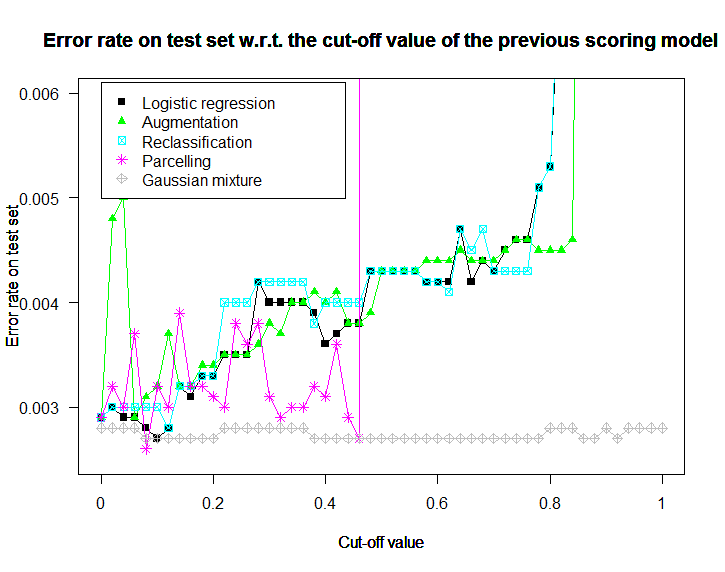
\includegraphics[width=0.4\textwidth]{figures/appendix/rejectinferencesimulation30var.png}
%\caption{Simulation of multivariate 30-dimensional Gaussian features and performance of various reject inference methods including the proposed generative approach.}
%\label{fig:simu_30var}
%\end{figure}


%\subsection{Reject inference methods applied to real data: previous experiments} \label{subsec:app_reject_real}
%
%This early work shows all reject inference methods based on \gls{lr} applied to various \gls{cacf} datasets: Electronics loans, Sports goods and Standard loans in Figure~\ref{fig:darty_reject},~\ref{fig:decathlon_reject} and~\ref{fig:M3_reject} respectively (beware: the colors / symbols do not correspond to the same methods in each graph). The acceptance / rejection mechanism $p_{\gls{phi}}(\gls{z} | \gls{bx})$ is again simulated using a \gls{lr}. Two things are striking in these figures: first, all methods perform relatively similarly and suffer a big performance drop once the acceptance rate is below 50 \% (at which point there are very few ``bad borrower'' events - $y = 0$); second, the multivariate generative model that performed best on simulated data in the previous section performs worst with real data, since it makes more hypotheses and is thus less flexible.
%
%\begin{figure}[H]
%\centering
%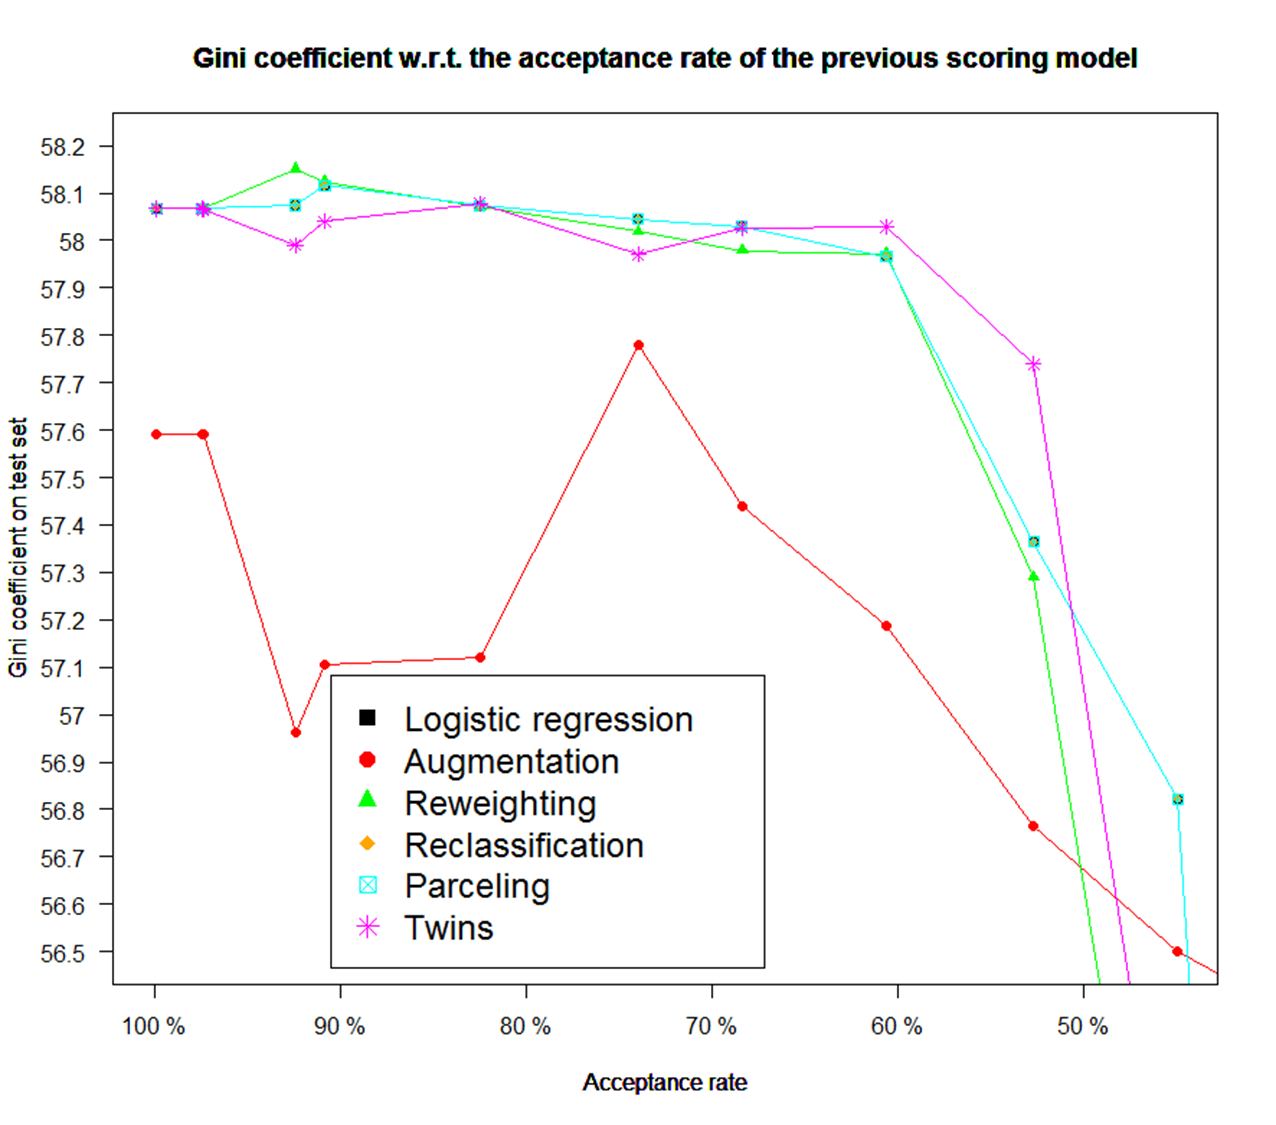
\includegraphics[width=0.4\textwidth]{figures/appendix/rejectinferencedarty3.png}
%\caption{Performance resulting from the use of reject inference methods in terms of Gini on an Electronics loans dataset from \gls{cacf}.}
%\label{fig:darty_reject}
%\end{figure}
%
%\begin{figure}[H]
%\centering
%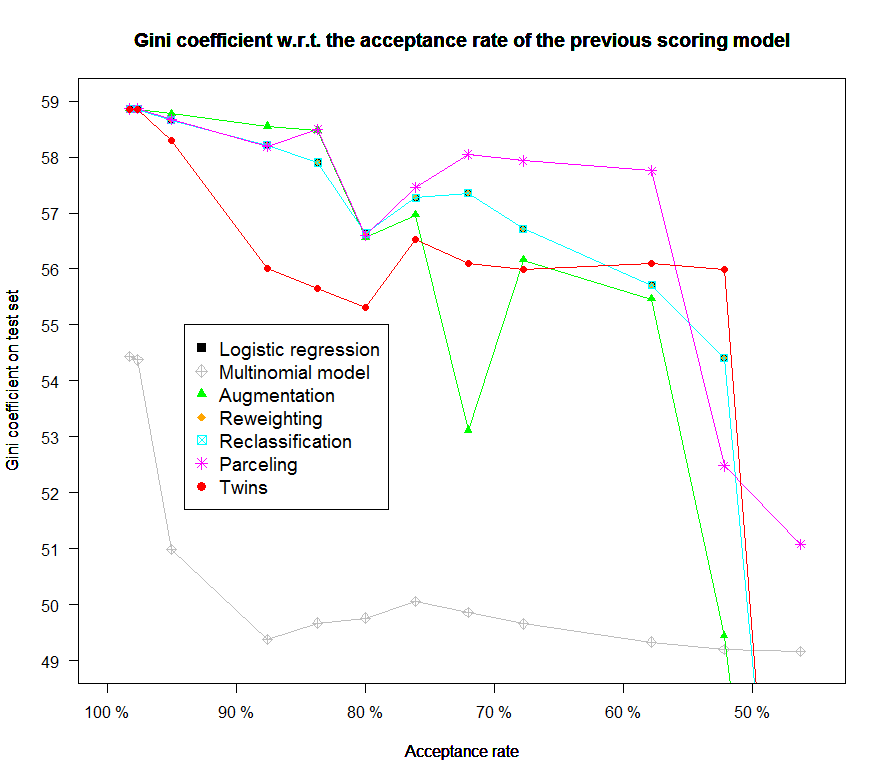
\includegraphics[width=0.4\textwidth]{figures/appendix/rejectinferencedecathlon.png}
%\caption{Performance resulting from the use of reject inference methods in terms of Gini on a Sports goods loans dataset from \gls{cacf}.}
%\label{fig:decathlon_reject}
%\end{figure}
%
%\begin{figure}[H]
%\centering
%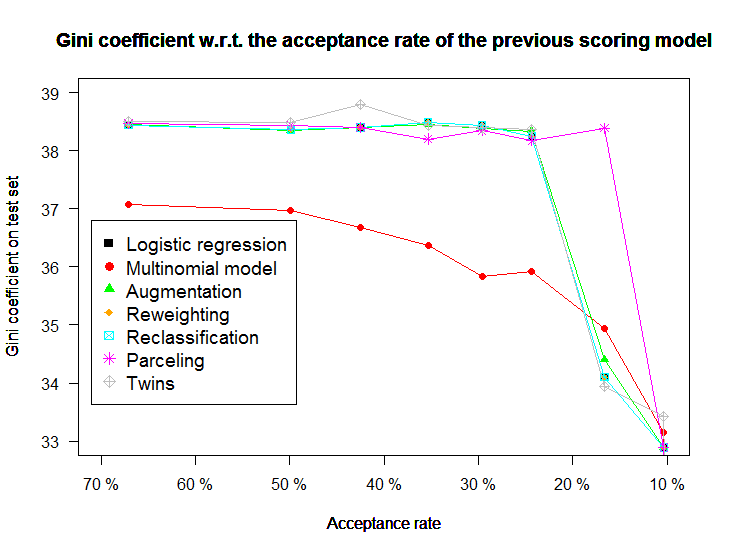
\includegraphics[width=0.4\textwidth]{figures/appendix/rejectinferenceM3.png}
%\caption{Performance resulting from the use of Reject Inference methods in terms of Gini on a Standard loans dataset from \gls{cacf}.}
%\label{fig:M3_reject}
%\end{figure}


\subsection{Performance of other predictive models w.r.t.\ the acceptance level} \label{subsec:app_reject_real_method}

Also part of an earlier work, this section's aim was to compare the performance of other ``machine learning'' models (although we purposely restricted our focus in Chapter~\ref{chap2} to the \gls{lr}) to see if, when presented with the same data and in presence of a simulated acceptance / rejection mechanism as earlier showcased, it would not be of better interest to switch to a different model, although it was argued in Chapter~\ref{chap2} that these models would not perform good under a \gls{mar} setting. The same datasets as in the previous section are used: the proposed models all perform poorer than \gls{lr} but most importantly their performance drops significantly with the proportion of simulated accepted clients. Some studies of the reject inference problem have focused on these ``machine learning'' models, see \textit{e.g.}\ \cite{guiza2014}.

\begin{figure}[H]
\centering
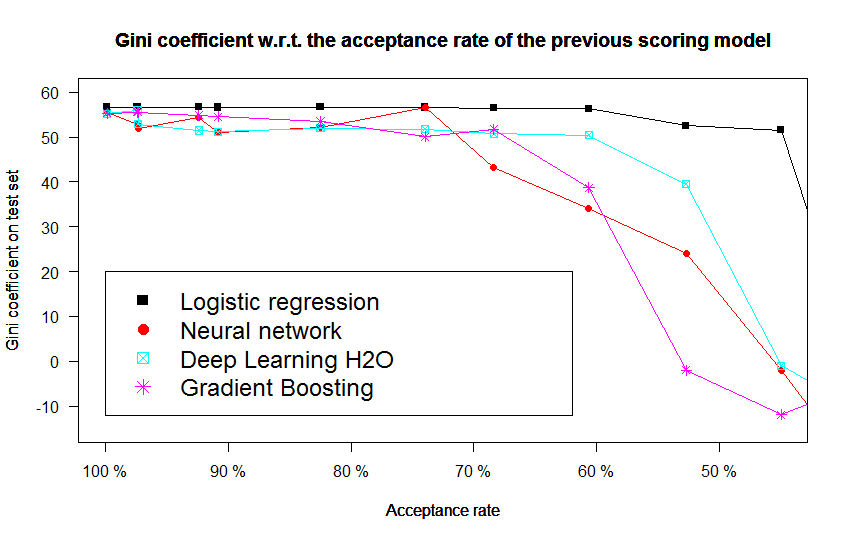
\includegraphics[width=0.4\textwidth]{figures/appendix/newmodelsdarty.png}
\caption{Performance resulting from the use of other predictive methods in terms of Gini on an Electronics loans dataset from \gls{cacf}.}
\label{fig:darty_othermodels}
\end{figure}

\begin{figure}[H]
\centering
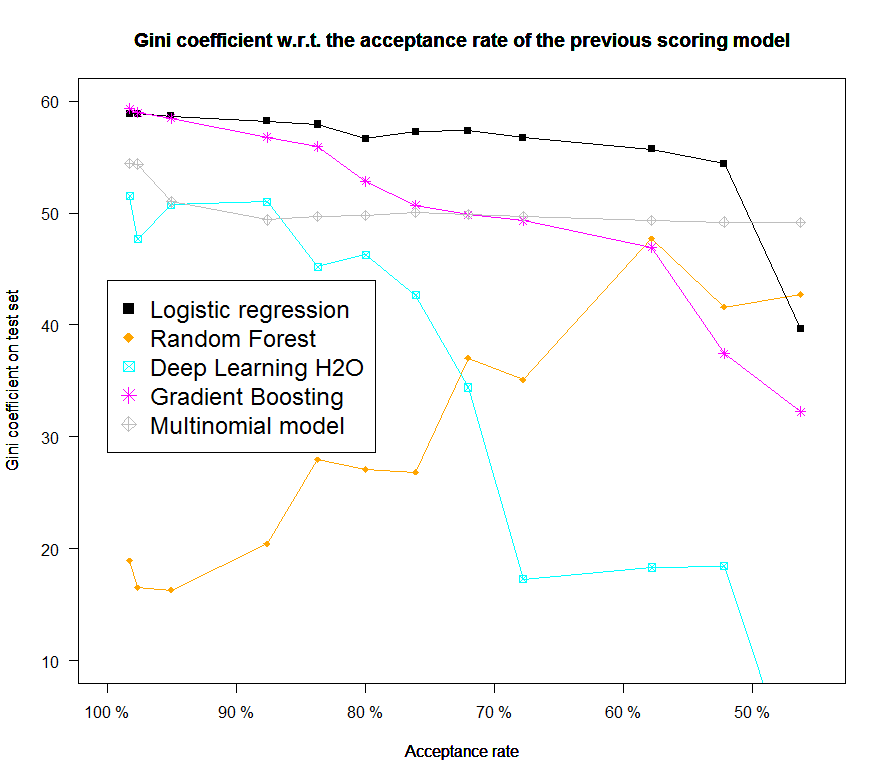
\includegraphics[width=0.4\textwidth]{figures/appendix/newmodelsdecathlon.png}
\caption{Performance resulting from the use of other predictive methods in terms of Gini on a Sports good loans dataset from \gls{cacf}.}
\label{fig:decathlon_othermodels}
\end{figure}

\begin{figure}[H]
\centering
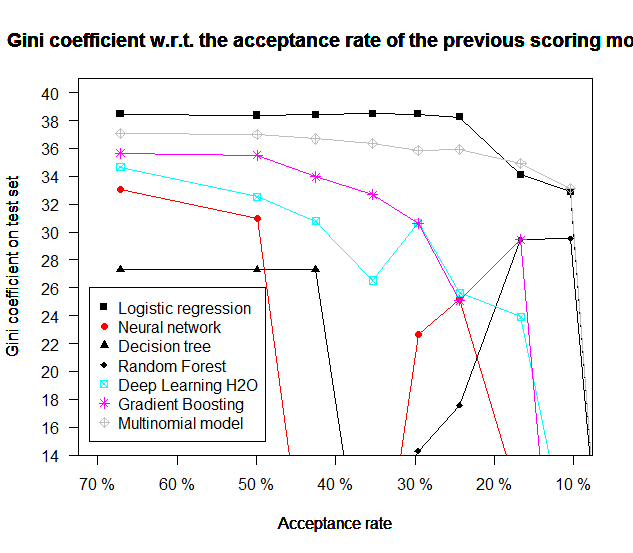
\includegraphics[width=0.4\textwidth]{figures/appendix/newmodelsm3web.png}
\caption{Performance resulting from the use of other predictive methods in terms of Gini on a Standard loans dataset from \gls{cacf}.}
\label{fig:M3_othermodels}
\end{figure}


\section{Discretization methods}

\subsection{Unsupervised methods}

\subsubsection{The \textit{equal-freq} algorithm}

The \textit{equal-freq} algorithm~\ref{equal-freq-disc} is illustrated on Figure~\ref{fig:disc_equal_freq}. 

\begin{figure}[H]
\centering
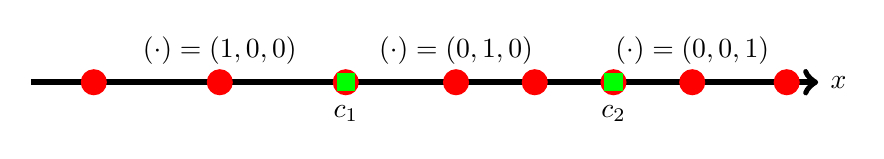
\begin{tikzpicture}[scale=0.2,every node/.style={scale=1}]
\draw[->,line width=0.08cm] (-12,0)--(38,0) node[right]{$\gls{x}$};

% Original data points
\node [red,circle, fill] at (-8,0) {};
\node [red,circle, fill] at (0,0) {};
\node [red,circle, fill] at (8,0) {};
\node [red,circle, fill] at (15,0) {};
\node [red,circle, fill] at (20,0) {};
\node [red,circle, fill] at (25,0) {};
\node [red,circle, fill] at (30,0) {};
\node [red,circle, fill] at (36,0) {};


% Cut points
\node [green,rectangle,rotate=90,fill] at (8,0) {};
\node [green,rectangle,rotate=90,fill] at (25,0) {};

\node at (8,-2) {$c_1$};
\node at (25,-2) {$c_2$};

% Disc value
\node at (0,2) {$\q(\cdot) = (1,0,0)$};
\node at (15,2) {$\q(\cdot) = (0,1,0)$};
\node at (30,2) {$\q(\cdot) = (0,0,1)$};


\end{tikzpicture}
\caption{\label{fig:disc_equal_freq} Original data in \textcolor{red}{red} is discretized using an \textit{equal-freq} procedure resulting in $m=3$ intervals using the two cutpoints in \textcolor{green}{green}.}
\end{figure}



\begin{algorithm}[H]
 \KwData{$n,\gls{bbx},\gls{bm} = (\gls{mj})_1^d$}
 \KwResult{$\hat{\q}$}
 \For{$j=1$ to $d$}{
Sort $\gls{bbx}_j$ by ascending order\;
Let $c_0=-\infty$, $c_{m_j} = + \infty$ and $c_{j,h} = x_{j,\left\lceil{{\frac{h \cdot n}{m_j}}}\right\rceil,j}$\;
Let $C_{j,h} = ]c_{j,h-1};c_{j,h}]$ and $\hat{\q}_j(\cdot) = (\hat{q}_{j,h}(\cdot))_1^{m_j}$\;
Set $\hat{q}_{j,h}(\cdot)=\mathds{1}_{C_{j,h}}(\cdot)$.
%\For{$i=1$ to $n$}{
%Set $q_i^j(x_j) = \begin{cases} 1 \text{ si } x_i^j \leq x_{\left\lceil{{\frac{n}{m_j}}}\right\rceil}^j \\ o \text{ si } x_{\left\lceil{{\frac{(o-1)*n}{m_j}}}\right\rceil}^j < x_i^j \leq x_{\left\lceil{{\frac{o*n}{m_j}}}\right\rceil}^j \\ m_j \text{ si } x_{\left\lceil{{\frac{(m_j-1)*n}{m_j}}}\right\rceil}^j < x_i^j \end{cases}$
%}
}
 \caption{\label{equal-freq-disc} \textit{equal-freq} discretization: an equal number of training observations are in each bin.}
\end{algorithm}


\subsubsection{The \textit{equal-length} algorithm} \label{app1:equal_length}

The \textit{equal-length} algorithm~\ref{equal-length-disc} is illustrated on Figure~\ref{fig:disc_equal_length}. 

\begin{figure}[H]
\centering
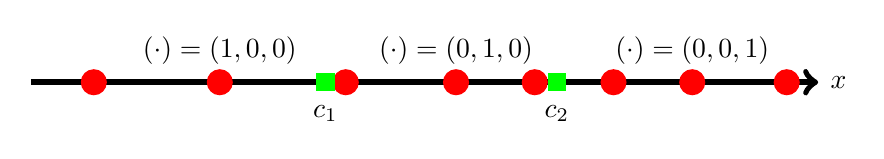
\begin{tikzpicture}[scale=0.2,every node/.style={scale=1}]
\draw[->,line width=0.08cm] (-12,0)--(38,0) node[right]{$\gls{x}$};

% Original data points
\node [red,circle, fill] at (-8,0) {};
\node [red,circle, fill] at (0,0) {};
\node [red,circle, fill] at (8,0) {};
\node [red,circle, fill] at (15,0) {};
\node [red,circle, fill] at (20,0) {};
\node [red,circle, fill] at (25,0) {};
\node [red,circle, fill] at (30,0) {};
\node [red,circle, fill] at (36,0) {};


% Cut points
\node [green,rectangle,rotate=90,fill] at (6.7,0) {};
\node [green,rectangle,rotate=90,fill] at (21.4,0) {};

\node at (6.7,-2) {$c_1$};
\node at (21.4,-2) {$c_2$};

% Disc value
\node at (0,2) {$\q(\cdot) = (1,0,0)$};
\node at (15,2) {$\q(\cdot) = (0,1,0)$};
\node at (30,2) {$\q(\cdot) = (0,0,1)$};


\end{tikzpicture}
\caption{\label{fig:disc_equal_length} Original data in \textcolor{red}{red} is discretized using an \textit{equal-length} procedure resulting in $m=3$ intervals using the two cutpoints in \textcolor{green}{green}.}
\end{figure}


\begin{algorithm}[H]
 \KwData{$n,\gls{bbx},\gls{bm} = (\gls{mj})_1^d$}
 \KwResult{$\hat{\q}$}
 \For{$j=1$ to $d$}{
Let $w_j = \max_{i} x_{i,j} - \min_{i} x_{i,j}$\;
Let $c_0=-\infty$, $c_{m_j} = + \infty$ and $c_{j,h} = \frac{w_j \cdot h}{m_j} + \min_{i} x_{i,j}$\;
Let $C_{j,h} = ]c_{j,h-1};c_{j,h}]$ and $\hat{\q}_j(\cdot) = (\hat{q}_{j,h}(\cdot))_1^{m_j}$\;
Set $\hat{q}_{j,h}(\cdot)=\mathds{1}_{C_{j,h}}(\cdot)$.
}
 \caption{\label{equal-length-disc} \textit{equal-length} discretization: each bin has the width of the training set's total support divided by the number of bins.}
\end{algorithm}



\subsection{Supervised univariate methods}

\subsubsection{The \textit{ChiMerge} algorithm}

\textit{ChiMerge}~\cite{kerber1992chimerge}, given in Algorithm~\ref{chimerge}, is a supervised (it takes into account the labels $\gls{bby}$) univariate (it does not take into account the other features $\gls{bbx}_{\{-j\}} = (\gls{bbx}_1, \dots, \gls{bbx}_{j-1}, \gls{bbx}_{j+1}, \dots, \gls{bbx}_d)$)). It is used indirectly in the benchmarks of Chapter~\ref{chap4} where we applied the same approach to categorical features by computing all the pairwise $\chi^2$ indepedence tests. Here we showcase a rather na\"{\i}ve implementation as a pseudo-code in Algorithm~\ref{chicollapse}, which in practice would perform poorly (because of exponential complexity in the number of categories $l_j$) but, from an iteration to another, a lot of $\chi^2$ tests are unaffected, so they can be stored rather than computed again. The initial and final steps of \textit{ChiMerge} are illustrated in Table~\ref{tab:chimerge_ex}. Refinements of the method, taking into account multiple testing and / or adapting the tests' siognificance level $\alpha$ to each feature, were done in~\cite{liu1995chi2,wang1998concurrent,tay2002modified,su2005extended}.

%\begin{table}
%\centering
%\caption{\label{tab:chimerge_ex} p-values of $\chi^2$ tests between subsequent categories. The pair of categories the least independent (\textit{i.e.}\ with highest p-value) is $(-\infty-18,18-20)$ which should be merged into $-\infty-20$.}
%\begin{tabular}{p{2.5cm}|p{2.5cm}|p{2.5cm}|p{2.5cm}}
%Category & \# samples & \# $\{Y=1\}$ & p-value \\
%\hline
%$-\infty$-18 & 10 & 5 & \multirow{2}{*}{\textbf{1}} \\
%18-20 & 10 & 5 & \multirow{2}{*}{0.3} \\
%20-22 & 10 & 6 & \multirow{2}{*}{0.2} \\
%22-24 & 10 & 4 & \multirow{2}{*}{0.2}\\
%24-$+\infty$ & 10 & 2 & \multirow{2}{*}{0.2} \\
%\dots & \dots & \dots & \dots \\
%\end{tabular}
%\end{table}
%
%\textcolor{red}{calculer les chi 2 exacts}

\begin{table}
\caption{\label{tab:chimerge_ex} p-values of $\chi^2$ tests between subsequent categories on the iris dataset.}
\centering
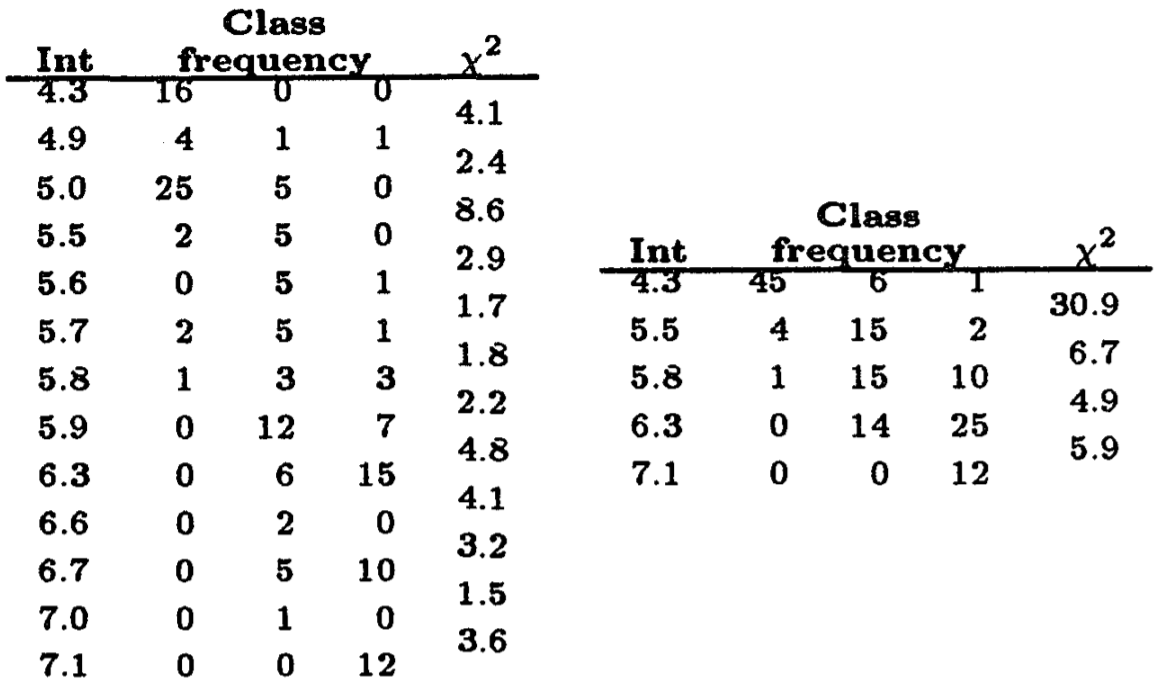
\includegraphics[width = .7\textwidth]{figures/appendix/tab_chimerge.PNG}
\end{table}

\begin{algorithm}[H]
 \KwData{$n,\gls{bbx},\alpha$}
 \KwResult{$\hat{\q}$}
 \For{$j=1$ to $d$}{
 $\alpha_{\text{max}}$ = 1\;
 Sort $\gls{bbx}_j$ in ascending order\;
 Let $c_0=-\infty$, $m_j = n$, $c_{m_j} = + \infty$ and $c_{j,h} = \frac{x_{i,j} + x_{i+1,j}}{2}$ for $1 \leq i \leq n-1$\;
 \While{$\alpha_{\text{max}} > \alpha$}{
Let $C_{j,h} = ]c_{j,h-1};c_{j,h}]$ and $\hat{\q}_j(\cdot) = (\hat{q}_{j,h}(\cdot))_1^{m_j}$\;
Set $\hat{q}_{j,h}(\cdot)=\mathds{1}_{C_{j,h}}(\cdot)$\;
%Perform $\chi^2$ tests of independence among all contiguous pairs\:
\For{$1 \leq h \leq m_j-1$}{
$\chi^2_h = \sum_{h'=h}^{h+1} \sum_{y=0}^{1} \frac{ \left( \sum_{i=1}^n \mathds{1}_{y}(y_i) \hat{q}_{j,h'}(x_{i,j} ) - \frac{\sum_{i=1}^n \hat{q}_{j,h'}(x_{i,j}) \times \sum_{i=1}^n \mathds{1}_{y}(y_i)}{n} \right)^2}{\frac{\sum_{i=1}^n \hat{q}_{j,h'}(x_{i,j}) \times \sum_{i=1}^n \mathds{1}_{y}(y_i)}{n}}$\;
}
%Under the null hypothesis that two consecutive intervals are independent w.r.t.\ the target $y$, $\chi^2_h$ is $\chi^2$-distributed (1 degree of freedom)\;
Let $c_{j,\argmin_h \chi^2_h} = \frac{c_{j,h} + c_{j,h+1}}{2}$ and $c_{j,h'} \leftarrow c_{j,h'+1}$ for $\argmin_h \chi^2_h < h' < m_j$\;
Let $m_j \leftarrow m_j-1$\;
Let $X \sim \chi^2$ and $\alpha_{\max} = \max_h p(X \geq \chi^2_h) = p(X \geq \min_h \chi^2_h)$.
}
}
 \caption{\label{chimerge} The ChiMerge algorithm discretizes features by performing $\chi^2$ tests recursively at a user-defined level $\alpha$.}
\end{algorithm}


\subsubsection{The \textit{MDLP} algorithm} \label{app1:mdlp}

The \textit{MDLP} algorithm~\cite{fayyad1993multi} is an entropy-based discretization method. Contrary to ChiMerge, where at the beginning all distinct values are put into separate categories and thereafter merged (bottom-up method), MDLP recursively calculates the entropy produced by each candidate cutpoint on their subsequent binary splits. It is reproduced in Algorithm~\ref{mdlp}.

\begin{algorithm}[H]
 \KwData{A continuous feature $\gls{bbx}_j$ which subscript $j$ is dropped in what follows; targets $\gls{bby}$.}
 \KwResult{Cutpoints $\mathcal{C}_\star$}
 Initialize $\mathcal{C}_\star = \varnothing$\;
Order $\gls{bbx}$\;
Compute the set $\mathcal{I}$ of indices $i$ such that $y_i \neq y_{i+1}$ (contiguous observations which are not of the same class)\;
Compute the set of candidate cutpoints $\mathcal{C}$ as the mean between these points, \textit{i.e.}\ $\mathcal{C} = \{\frac{x_i + x_{i+1}}{2} | i \in \mathcal{I} \}$\;
Compute the class entropy of each candidate cutpoint $c \in \mathcal{C}$ as:
\[ \text{E}(c) = \frac{|\gls{bbx} < c|}{|\gls{bbx}|} \text{Ent}(\gls{bbx} < c) + \frac{|\gls{bbx} > c|}{|\gls{bbx}|} \text{Ent}(\gls{bbx} > c), \]
where $\text{Ent}(\gls{bbx} < c) = - \sum_{y=0}^1 p(y,\gls{bbx} < c) \ln p(y,\gls{bbx} < c)$ and $p$ is estimated \textit{via} class proportions, \textit{i.e.}\ $p(y,\gls{bbx} < c) = \frac{|\{i | y_i = y \& x_i < c \}|}{|\gls{bbx} < c|}$\;
Select $c_\star$ which minimizes $\text{E}(c)$ and append it to $\mathcal{C}_\star$\;
Repeat steps for $\{\gls{bbx}< c\}$ and $\{\gls{bbx} > c\}$\;
Stop when $\text{Gain}(c,\gls{bbx}) = \text{E}(c) - \text{Ent}(\gls{bbx}) \leq \frac{\ln_2 (|\gls{bbx}|-1)}{|\gls{bbx}|} + \frac{\Delta(c,\gls{bbx}) }{|\gls{bbx}|}$ where $\Delta(c,\gls{bbx}) = \ln_2 7 - (k \text{Ent}(\gls{bbx}) - k_{<c}\text{Ent}(\gls{bbx} < c) - k_{>c}\text{Ent}(\gls{bbx} < c))$ and $k$, $k_{<c}$, $k_{>c}$ represent the number of classes (1 or 2 in the binary setting) in their respective sample $\gls{bbx}$, $\gls{bbx} < c$ and $\gls{bbx} > c$\;
 \caption{\label{mdlp} The MDLP algorithm recursively performs discretization with an information gain criterion.}
\end{algorithm}


\subsection{Proposal: \textit{glmdisc}}


\subsubsection{\textit{glmdisc} with neural networks} \label{app1:glmdiscNN}

This section describes the \textit{glmdisc}-NN algorithm developed in Chapter~\ref{chap4} and examplifies it on simulated data in Figure~\ref{fig:animNN}.

\begin{algorithm}[H]
 \KwData{$((\gls{bbx}_j)_1^{d}, \gls{bby}),S,\bm{m}_\text{start}$}
 \KwResult{$\hat{\q}^{(s^\star)}$}
 Initialization of the network: for each feature feature $j$, add a softmax with $m_{j,\text{start}}$ outputs which are themselves combined in a sigmoid neuron\;
 Initialization of the network's weights at random\;
 $s = 0$\;
 \While{$s < S$}{
Perform feed-forward pass of the data: calculate $p_{\gls{bth}^{(s)}}(\gls{bby} | \q_{\ag^{(s)}}(\gls{bbx}))$\;
Perform back-propagation of the error via Stochastic Gradient Descent which yields parameters $(\gls{bth}^{(s+1)},\ag^{(s+1)})$\;
 Compute the \textit{maximum a posteriori} of the hidden layer's representations $\hat{\q}^{(s)}(\gls{bbx})$ such that $\hat{q}_{j,h}(x_j) = 1 \text{ if } h = \argmax_{1 \leq h' \leq m_j} q_{\hat{\ag}_{j,h'}}, 0 \text{ otherwise.}$\;
 Compute the associated \gls{lr} parameters $\hat{\gls{bth}}^{(s)} = \argmax_{\gls{bth}} \ell(\gls{bth} ; {\hat{\q}_j^{(s)}}, \gls{bby})$\;
    $s \leftarrow s+1$\;
}
 Choose the best quantization $\hat{\q}^{(s^\star)}$, which associated \gls{lr} parameters yield the lowest BIC criterion\;
 \caption{\label{NN-disc} \textit{glmdisc}-NN: supervised multivariate quantization for logistic regression with neural networks.}
\end{algorithm}

\begin{figure}[!h]
\begin{animateinline}[poster=first, controls=all, palindrome, autopause, autoresume, width=\textwidth, height=6cm]{3}
\multiframe{200}{i=1+1}{\input{R_CODE_FIGURES/appendix/animation_disc_tensorflow/False_simulated_data/feature_0_iteration_\i.tex}}%
\end{animateinline}
\caption{\label{fig:animNN} Animation of the softmax activation functions $\q_{\ag^{(s)}}$ over the epoch $(s)$.}
\end{figure}


%\textcolor{red}{à décommenter // ajouter caption}

\subsubsection{\textit{glmdisc} with an \gls{sem} algorithm} \label{app1:glmdiscSEM}

This section describes the \textit{glmdisc}-SEM algorithm developed in Chapter~\ref{chap4} and examplifies it on simulated data in Figure~\ref{fig:animSEM}.

\begin{algorithm}[H]
 \KwData{$((\gls{bbx}_j)_1^{d}, \gls{bby}),S,\bm{m}_\text{start}$}
 \KwResult{$\hat{\bbqk}^{(s^\star)}$}
 Initialization of $\bbqk_j^{(0)}$ at random in $\{1, \dots, m_{j,\text{start}}\}$ and one-hot encode the resulting vector\;
 $s = 0$\;
 \While{$s < S$}{
  Adjust logistic regression $\gls{bth}^{(s)} = \argmax_{\gls{bth}} \ell(\gls{bth};\bbqk^{(s)}, \gls{bby})$\;
  \For{$j = 1$ \KwTo $d$}{
   Adjust multinomial logistic regression or contingency tables $\ag_j^{(s)} = \argmax_{\ag_j} \ell(\ag_j;\gls{bbx}_j,\bbqk_j^{(s)})$\;
Draw new latent features ${\bqk_j^{(s+1)}} \sim \text{ Mult} \left( p_{\gls{bth}^{(s)}}(y | \bqk^{(s)}_{-\{ j \}}, \cdot) p_{\ag_j^{(s)}}(\cdot | \gls{bx}_j) \right)$ for each observation (the subscript $i$ is voluntarily omitted)\;
 Compute the \textit{maximum a posteriori} of these latent features for all observations ${\hat{\bqk}_j^{(s)}} = \argmax_{\bqk_j} p_{\ag_j^{(s)}}(\bqk_j | \gls{bx}_j)$\;
 Compute the associated \gls{lr} parameters $\hat{\gls{bth}}^{(s)} = \argmax_{\gls{bth}} \ell(\gls{bth} ; {\hat{\bbqk}_j^{(s)}}, \gls{bby})$\;
   }
   $s \leftarrow s+1$\;
 }
 Choose the best quantization $\hat{\bbqk}^{(s^\star)}$, which associated \gls{lr} parameters $\hat{\gls{bth}}^{(s_\star)}$ yield the lowest BIC criterion.
 \caption{\label{SEM-disc} \textit{glmdisc}-SEM: supervised multivariate quantization for logistic regression with an \gls{sem} algorithm.}
\end{algorithm}

\begin{figure}[!h]
\begin{animateinline}[poster=first, controls=all, palindrome, autopause, autoresume, width=\textwidth, height=9.5cm]{5}
\multiframe{200}{i=1+1}{\input{R_CODE_FIGURES/appendix/animation_disc_SEM/sem_simulated_data/sem_feature_1_iter_\i.tex}}%
\end{animateinline}
\caption{\label{fig:animSEM} Animation of the $\bqk_j$ of \textit{glmdisc}-SEM through the iterations $(s)$.}
\end{figure}

%\textcolor{red}{à décommenter // ajouter caption  et numéro itération}


\section{Factor levels grouping method} \label{app1:chicollapse}

As part of Chapter~\ref{chap4}, we gave results for competing methods MDLP / $\chi^2$ tests where the $\chi^2$ tests can be explicited in Algorithm~\ref{chicollapse} which I called ChiCollapse. My rather na{\"\i}ve implementation (where, as in the pseudo-code, all pairwise $\chi^2$ tests are recalculated at each step) is available as a gist on Github at \url{https://gist.github.com/adimajo/eb007492007d650091f6bd7cb2047493}. An example of the resulting usage of the grouped levels in a predictive setting is also given as a gist on Github at \url{https://gist.github.com/adimajo/8f8401b59ba838c65534673842b0f60d}.

\begin{algorithm}[H]
 \KwData{$n,\gls{bbx},\alpha$}
 \KwResult{$\hat{\q}$}
 \For{$j=1$ to $d$}{
 $\alpha_{\text{max}}$ = 1\;
 Let $C_{j,h} = \{h\}$ for $1 \leq i \leq l_j$\;
 \While{$\alpha_{\text{max}} > \alpha$}{
Let $\hat{\q}_j(\cdot) = (\hat{q}_{j,h}(\cdot))_1^{m_j}$\;
Set $\hat{q}_{j,h}(\cdot)=\mathds{1}_{C_{j,h}}(\cdot)$\;
%Perform all pairwise $\chi^2$ tests of independence among all contiguous pairs\:
\For{$1 \leq h_1 < h_2 \leq m_j$}{
$\chi^2_{h_1,h_2} = \sum_{h'=h_1}^{h_2} \sum_{y=0}^{1} \frac{ \left( \sum_{i=1}^n \mathds{1}_{y}(y_i) \hat{q}_{j,h'}(x_{i,j} ) - \frac{\sum_{i=1}^n \hat{q}_{j,h'}(x_{i,j}) \times \sum_{i=1}^n \mathds{1}_{y}(y_i)}{n} \right)^2}{\frac{\sum_{i=1}^n \hat{q}_{j,h'}(x_{i,j}) \times \sum_{i=1}^n \mathds{1}_{y}(y_i)}{n}}$\;}
%Under the null hypothesis that two factor levels are independent w.r.t.\ the target $y$, $\chi^2_{h_1,h_2}$ is $\chi^2$-distributed (1 degree of freedom)\;
Let $(h_1,h_2) = \argmin_{h_1,h_2} \chi^2_{h_1,h_2}$, $C_{j,h_1} = C_{j,h_1} \cup C_{j,h_2}$ and $C_{j,h} \leftarrow C_{j,h+1}$ for $h_2 \leq h < m_j$\;
Let $m_j \leftarrow m_j-1$\;
Let $X \sim \chi^2$ and $\alpha_{\max} = \max_{h_1,h_2} p(X \geq \chi^2_{h_1,h_2}) = p(X \geq \min_{h_1,h_2} \chi^2_{h_1,h_2})$.
}
}
 \caption{\label{chicollapse} ChiCollapse algorithm: adaptation of ChiMerge to categorical features.}
\end{algorithm}


%\section{Interaction discovery methods}



\section{Logistic regression-based trees}


%\subsection{\gls{pca}} \label{app1:sec_pca}
%
%\begin{algorithm}[H]
% \KwData{$\gls{bbx}$}
% \KwResult{$\gls{bbx}$}
%
% \caption{\label{alg:pca} \gls{pca} algorithm.}
%\end{algorithm}

%\subsection{\gls{mca}} \label{app1:sec_mca}
%
%\begin{algorithm}[H]
% \KwData{$n,\gls{bbx},\alpha$}
% \KwResult{$\hat{\q}$}
%
% \caption{\label{alg:mca} \gls{mca} algorithm.}
%\end{algorithm}


%\subsection{\gls{famd}} \label{app1:sec_famd}
%
%\begin{algorithm}[H]
% \KwData{$n,\gls{bbx},\alpha$}
% \KwResult{$\hat{\q}$}
%
% \caption{\label{alg:famd} \gls{famd} algorithm.}
%\end{algorithm}


\subsection{LogitBoost} \label{LogitBoost}

The LogitBoost algorithm~\cite{friedman2000additive} for 2 classes is equivalent to the Iterative Reweighted Least Squares method~\cite{friedman2001elements}. However, in \gls{lmt}, in order to perform feature selection, a slight modification is brought to the algorithm so as to fit univariate regressions and pick the best. It is given in Algorithm~\ref{alg:logitboost}.

\begin{algorithm}[H]
 \KwData{$n,\gls{bbx},\gls{bby}, S$}
 \KwResult{$F(\gls{bx})$}
Let weights $w_i = 1 / n$, $F(x) = 0$, $p(1 | \gls{bx}) = \frac{\exp(F(\gls{bx})}{\exp(F(\gls{bx}) + \exp(-F(\gls{bx})}$\;
\For{$s = 1$ to $S$}{
Compute weights $\mathbf{w} = p(1 | \gls{bbx}) \odot (\mathbf{1} - p(1 | \gls{bbx}))$\;
Compute response $z_{i} = \frac{y_i - p(1 | \gls{bx})}{w_i}$\;
\For{$j = 1$ to $d$}{
Fit the univariate reweighted regression coefficient $\hat{\theta}_{s,j} = \argmin_\theta \sum_{i=1}^n w_i \cdot (z_i - \theta x_{i,j})^2 $\;
}
Retrieve the best univariate coefficient $j^{\star} = \argmin_{1 \leq j \leq d} \sum_{i=1}^n w_i \cdot (z_i - \hat{\theta}_{s,j} x_{i,j})^2 $\;
Update $F(\gls{bx}) = F(\gls{bx}) + \frac{1}{2} \hat{\theta}_{s,j^\star} x_j$\;
}
 \caption{\label{alg:logitboost} LogitBoost algorithm.}
\end{algorithm}


\subsection{\gls{pls}} \label{app1:sec_pls}

The \gls{pls} algorithm given in~\eqref{alg:pls} has been proposed in~\cite{wold1984collinearity}. This version is adapted from~\cite{friedman2001elements} (Algorithm 3.3 in Section 3.5.2 p.\ 81).

\begin{algorithm}[H]
 \KwData{$\gls{bbx},\gls{bby}$}
 \KwResult{$\mathbf{z}$}
Standardize each $\gls{bbx}_j$ to have mean zero and variance one (which implies that categorical features have been one-hot encoded prior to this step) \;
Set $\hat{\gls{bby}}^{(0)} = \mathbf{1}' |\gls{bby}|$\;
Set $\gls{bbx}_j^{(0)} = \gls{bbx}_j$\;
\For{$j=1$ to $d$}{
Let $\mathbf{z}_j = \sum_{j {'} = 1}^d \hat{\phi}_{j,j {'} } \gls{bbx}_{j {'} }^{(j-1)}$ where $\hat{\phi}_{j,j {'} } = \gls{bbx}_{j {'} }^{(j-1)} {'} \gls{bby}$ \;
Let $\theta_j = \frac{\mathbf{z}_j {'} \gls{bby}}{\mathbf{z}_j {'} \mathbf{z}_j}$\;
Let $\hat{\gls{bby}}^{(j)} = \hat{\gls{bby}}^{(j-1)} + \theta_j \mathbf{z}_j$\;
Orthogonalize each $\gls{bbx}_{j{'}}^{(j-1)}$ w.r.t.\ $\mathbf{z}_j$: $\gls{bbx}_{j{'}}^{(j)} = \gls{bbx}_{j{'}}^{(j-1)} - \frac{\mathbf{z}_j {'} \gls{bbx}_{j{'}}^{(j-1)}}{\mathbf{z}_{j} {'} \mathbf{z}_j} \mathbf{z}_j$ for $1 \leq j{'} \leq d$\;
}
 \caption{\label{alg:pls} \gls{pls} algorithm (adapted from~\cite{friedman2001elements}).}
\end{algorithm}


\subsection{\gls{spc}} \label{app1:sec_spc}

The \gls{spc} algorithm given in~\eqref{alg:spc} has been proposed in~\cite{bair2006prediction}. This version is adapted from~\cite{friedman2001elements} (Algorithm 18.1 in Section 18.6. p.\ 678).

\begin{algorithm}[H]
 \KwData{$\gls{bbx},\gls{bby},\{ T_1, \dots, T_K \}, \{ m_1, \dots, m_L \}$}
 \KwResult{$\mathbf{z}$}
Standardize each $\gls{bbx}_j$ to have mean zero and variance one (which implies that categorical features have been one-hot encoded prior to this step) \;
Compute the univariate regression coefficients for the outcomes $\gls{bby}$ as a function of each features $\gls{bbx}_j$\;
\For{Principal components $m \in \{ m_1, \dots, m_L \}$}{
\For{Threshold $T \in \{ T_1, \dots, T_K \}$}{
Form a reduced data matrix consisting of only those features whose univariate coefficient exceeds $T$ in absolute value, and compute the first $m$ principal components of this matrix\;
Use these principal components in a \gls{lr} model to predict the outcomes $\gls{bby}$\;
} 
}
Pick $(T^\star, m^\star)$ by cross-validation.
 \caption{\label{alg:spc} \gls{spc} algorithm (adapted from~\cite{friedman2001elements}).}
\end{algorithm}

\subsection{\gls{lmt}} \label{app1:sec_lmt}

The \gls{lmt} algorithm given in~\eqref{alg:lmt} has been proposed in~\cite{landwehr2005logistic}.

\begin{algorithm}[H]
 \KwData{$\gls{bbx}, \gls{bby}$}
 \KwResult{The logistic regression tree}
 Fit a classification tree using the C4.5 algorithm\;
 Fit a \gls{lr} at the root node by using LogitBoost (Algorithm~\ref{alg:logitboost} - the number of iterations is determined by cross-validation)\;
 Fit a \gls{lr} at the children nodes by resuming LogitBoost (Algorithm~\ref{alg:logitboost}) on the respective sub-populations\;
 Prune the tree based on the CART algorithm's pruning criterion (composed of misclassification error and complexity penalization)\;
 \caption{\label{alg:lmt} \gls{lmt} algorithm (adapted from~\cite{landwehr2005logistic}).}
\end{algorithm}

\subsection{\gls{mob}} \label{app1:sec_mob}

The \gls{mob} algorithm given in~\eqref{alg:mob} has been proposed in~\cite{zeileis2008model}.

\begin{algorithm}[H]
 \KwData{$\gls{bbx}, \gls{bby}$}
 \KwResult{The logistic regression tree}
 Fit a \gls{lr} to all observations in current node\;
 Test for ``parameters instability'' for all features $x_j \in \gls{bx}$\;
 If the minimum p-value of these tests is lower than a user-defined threshold, the process is recursively repeated on the children nodes defined by this feature\;
 \caption{\label{alg:mob} \gls{mob} algorithm (adapted from~\cite{zeileis2008model}).}
\end{algorithm}

\printbibliography[heading=subbibliography, title=References of Appendix A]
